\documentclass[twoside]{book}

% Packages required by doxygen
\usepackage{fixltx2e}
\usepackage{calc}
\usepackage{doxygen}
\usepackage[export]{adjustbox} % also loads graphicx
\usepackage{graphicx}
\usepackage[utf8]{inputenc}
\usepackage{makeidx}
\usepackage{multicol}
\usepackage{multirow}
\PassOptionsToPackage{warn}{textcomp}
\usepackage{textcomp}
\usepackage[nointegrals]{wasysym}
\usepackage[table]{xcolor}

% Font selection
\usepackage[T1]{fontenc}
\usepackage[scaled=.90]{helvet}
\usepackage{courier}
\usepackage{amssymb}
\usepackage{sectsty}
\renewcommand{\familydefault}{\sfdefault}
\allsectionsfont{%
  \fontseries{bc}\selectfont%
  \color{darkgray}%
}
\renewcommand{\DoxyLabelFont}{%
  \fontseries{bc}\selectfont%
  \color{darkgray}%
}
\newcommand{\+}{\discretionary{\mbox{\scriptsize$\hookleftarrow$}}{}{}}

% Page & text layout
\usepackage{geometry}
\geometry{%
  a4paper,%
  top=2.5cm,%
  bottom=2.5cm,%
  left=2.5cm,%
  right=2.5cm%
}
\tolerance=750
\hfuzz=15pt
\hbadness=750
\setlength{\emergencystretch}{15pt}
\setlength{\parindent}{0cm}
\setlength{\parskip}{3ex plus 2ex minus 2ex}
\makeatletter
\renewcommand{\paragraph}{%
  \@startsection{paragraph}{4}{0ex}{-1.0ex}{1.0ex}{%
    \normalfont\normalsize\bfseries\SS@parafont%
  }%
}
\renewcommand{\subparagraph}{%
  \@startsection{subparagraph}{5}{0ex}{-1.0ex}{1.0ex}{%
    \normalfont\normalsize\bfseries\SS@subparafont%
  }%
}
\makeatother

% Headers & footers
\usepackage{fancyhdr}
\pagestyle{fancyplain}
\fancyhead[LE]{\fancyplain{}{\bfseries\thepage}}
\fancyhead[CE]{\fancyplain{}{}}
\fancyhead[RE]{\fancyplain{}{\bfseries\leftmark}}
\fancyhead[LO]{\fancyplain{}{\bfseries\rightmark}}
\fancyhead[CO]{\fancyplain{}{}}
\fancyhead[RO]{\fancyplain{}{\bfseries\thepage}}
\fancyfoot[LE]{\fancyplain{}{}}
\fancyfoot[CE]{\fancyplain{}{}}
\fancyfoot[RE]{\fancyplain{}{\bfseries\scriptsize Generated by Doxygen }}
\fancyfoot[LO]{\fancyplain{}{\bfseries\scriptsize Generated by Doxygen }}
\fancyfoot[CO]{\fancyplain{}{}}
\fancyfoot[RO]{\fancyplain{}{}}
\renewcommand{\footrulewidth}{0.4pt}
\renewcommand{\chaptermark}[1]{%
  \markboth{#1}{}%
}
\renewcommand{\sectionmark}[1]{%
  \markright{\thesection\ #1}%
}

% Indices & bibliography
\usepackage{natbib}
\usepackage[titles]{tocloft}
\setcounter{tocdepth}{3}
\setcounter{secnumdepth}{5}
\makeindex

% Hyperlinks (required, but should be loaded last)
\usepackage{ifpdf}
\ifpdf
  \usepackage[pdftex,pagebackref=true]{hyperref}
\else
  \usepackage[ps2pdf,pagebackref=true]{hyperref}
\fi
\hypersetup{%
  colorlinks=true,%
  linkcolor=blue,%
  citecolor=blue,%
  unicode%
}

% Custom commands
\newcommand{\clearemptydoublepage}{%
  \newpage{\pagestyle{empty}\cleardoublepage}%
}

\usepackage{caption}
\captionsetup{labelsep=space,justification=centering,font={bf},singlelinecheck=off,skip=4pt,position=top}

%===== C O N T E N T S =====

\begin{document}

% Titlepage & ToC
\hypersetup{pageanchor=false,
             bookmarksnumbered=true,
             pdfencoding=unicode
            }
\pagenumbering{alph}
\begin{titlepage}
\vspace*{7cm}
\begin{center}%
{\Large My Project }\\
\vspace*{1cm}
{\large Generated by Doxygen 1.8.14}\\
\end{center}
\end{titlepage}
\clearemptydoublepage
\pagenumbering{roman}
\tableofcontents
\clearemptydoublepage
\pagenumbering{arabic}
\hypersetup{pageanchor=true}

%--- Begin generated contents ---
\chapter{Namespace Index}
\section{Namespace List}
Here is a list of all namespaces with brief descriptions\+:\begin{DoxyCompactList}
\item\contentsline{section}{\mbox{\hyperlink{namespace_ui}{Ui}} }{\pageref{namespace_ui}}{}
\end{DoxyCompactList}

\chapter{Hierarchical Index}
\section{Class Hierarchy}
This inheritance list is sorted roughly, but not completely, alphabetically\+:\begin{DoxyCompactList}
\item \contentsline{section}{Abstract\+Stage\+Factory}{\pageref{class_abstract_stage_factory}}{}
\begin{DoxyCompactList}
\item \contentsline{section}{Stage\+One\+Factory}{\pageref{class_stage_one_factory}}{}
\item \contentsline{section}{Stage\+Two\+Factory}{\pageref{class_stage_two_factory}}{}
\end{DoxyCompactList}
\item \contentsline{section}{Ball}{\pageref{class_ball}}{}
\begin{DoxyCompactList}
\item \contentsline{section}{Ball\+Decorator}{\pageref{class_ball_decorator}}{}
\begin{DoxyCompactList}
\item \contentsline{section}{Ball\+Smash\+Decorator}{\pageref{class_ball_smash_decorator}}{}
\item \contentsline{section}{Ball\+Sparkle\+Decorator}{\pageref{class_ball_sparkle_decorator}}{}
\item \contentsline{section}{Cue\+Ball}{\pageref{class_cue_ball}}{}
\end{DoxyCompactList}
\item \contentsline{section}{Composite\+Ball}{\pageref{class_composite_ball}}{}
\item \contentsline{section}{Stage\+One\+Ball}{\pageref{class_stage_one_ball}}{}
\end{DoxyCompactList}
\item \contentsline{section}{Ball\+Smash\+Decorator\+:\+:Crumb}{\pageref{struct_ball_smash_decorator_1_1_crumb}}{}
\item \contentsline{section}{Game}{\pageref{class_game}}{}
\item \contentsline{section}{Game\+Builder}{\pageref{class_game_builder}}{}
\begin{DoxyCompactList}
\item \contentsline{section}{Stage\+One\+Builder}{\pageref{class_stage_one_builder}}{}
\item \contentsline{section}{Stage\+Two\+Builder}{\pageref{class_stage_two_builder}}{}
\end{DoxyCompactList}
\item \contentsline{section}{Game\+Director}{\pageref{class_game_director}}{}
\item \contentsline{section}{Pocket}{\pageref{class_pocket}}{}
\item Q\+Dialog\begin{DoxyCompactList}
\item \contentsline{section}{Dialog}{\pageref{class_dialog}}{}
\end{DoxyCompactList}
\item \contentsline{section}{Ball\+Sparkle\+Decorator\+:\+:Sparkle}{\pageref{struct_ball_sparkle_decorator_1_1_sparkle}}{}
\item \contentsline{section}{Table}{\pageref{class_table}}{}
\begin{DoxyCompactList}
\item \contentsline{section}{Stage\+One\+Table}{\pageref{class_stage_one_table}}{}
\item \contentsline{section}{Stage\+Two\+Table}{\pageref{class_stage_two_table}}{}
\end{DoxyCompactList}
\end{DoxyCompactList}

\chapter{Class Index}
\section{Class List}
Here are the classes, structs, unions and interfaces with brief descriptions\+:\begin{DoxyCompactList}
\item\contentsline{section}{\mbox{\hyperlink{class_abstract_stage_factory}{Abstract\+Stage\+Factory}} }{\pageref{class_abstract_stage_factory}}{}
\item\contentsline{section}{\mbox{\hyperlink{class_add_ball_command}{Add\+Ball\+Command}} }{\pageref{class_add_ball_command}}{}
\item\contentsline{section}{\mbox{\hyperlink{class_ball}{Ball}} }{\pageref{class_ball}}{}
\item\contentsline{section}{\mbox{\hyperlink{class_ball_decorator}{Ball\+Decorator}} \\*The \mbox{\hyperlink{class_ball_decorator}{Ball\+Decorator}} class This acts as a Decorator. Any methods not overriden can simply forward the requests onto the Class this is decorated }{\pageref{class_ball_decorator}}{}
\item\contentsline{section}{\mbox{\hyperlink{class_ball_smash_decorator}{Ball\+Smash\+Decorator}} }{\pageref{class_ball_smash_decorator}}{}
\item\contentsline{section}{\mbox{\hyperlink{class_ball_sparkle_decorator}{Ball\+Sparkle\+Decorator}} }{\pageref{class_ball_sparkle_decorator}}{}
\item\contentsline{section}{\mbox{\hyperlink{class_command}{Command}} }{\pageref{class_command}}{}
\item\contentsline{section}{\mbox{\hyperlink{class_composite_ball}{Composite\+Ball}} }{\pageref{class_composite_ball}}{}
\item\contentsline{section}{\mbox{\hyperlink{struct_ball_smash_decorator_1_1_crumb}{Ball\+Smash\+Decorator\+::\+Crumb}} }{\pageref{struct_ball_smash_decorator_1_1_crumb}}{}
\item\contentsline{section}{\mbox{\hyperlink{class_cue_ball}{Cue\+Ball}} \\*The \mbox{\hyperlink{class_cue_ball}{Cue\+Ball}} class This handles some mouse interactions, and can control the position/velocity of the ball The ball will only be able to be controlled if the mouse click\&drag event originated at the position of the cue ball }{\pageref{class_cue_ball}}{}
\item\contentsline{section}{\mbox{\hyperlink{class_dialog}{Dialog}} }{\pageref{class_dialog}}{}
\item\contentsline{section}{\mbox{\hyperlink{class_game}{Game}} }{\pageref{class_game}}{}
\item\contentsline{section}{\mbox{\hyperlink{class_game_builder}{Game\+Builder}} }{\pageref{class_game_builder}}{}
\item\contentsline{section}{\mbox{\hyperlink{class_game_director}{Game\+Director}} }{\pageref{class_game_director}}{}
\item\contentsline{section}{\mbox{\hyperlink{class_game_state_caretaker}{Game\+State\+Caretaker}} }{\pageref{class_game_state_caretaker}}{}
\item\contentsline{section}{\mbox{\hyperlink{class_game_state_memento}{Game\+State\+Memento}} \\*
\begin{DoxyItemize}
\item the memento owns all the variable that is in the game 
\end{DoxyItemize}}{\pageref{class_game_state_memento}}{}
\item\contentsline{section}{\mbox{\hyperlink{class_invoker}{Invoker}} }{\pageref{class_invoker}}{}
\item\contentsline{section}{\mbox{\hyperlink{class_pocket}{Pocket}} }{\pageref{class_pocket}}{}
\item\contentsline{section}{\mbox{\hyperlink{class_replace_cue_ball_command}{Replace\+Cue\+Ball\+Command}} }{\pageref{class_replace_cue_ball_command}}{}
\item\contentsline{section}{\mbox{\hyperlink{struct_ball_sparkle_decorator_1_1_sparkle}{Ball\+Sparkle\+Decorator\+::\+Sparkle}} }{\pageref{struct_ball_sparkle_decorator_1_1_sparkle}}{}
\item\contentsline{section}{\mbox{\hyperlink{class_stage_one_ball}{Stage\+One\+Ball}} }{\pageref{class_stage_one_ball}}{}
\item\contentsline{section}{\mbox{\hyperlink{class_stage_one_builder}{Stage\+One\+Builder}} }{\pageref{class_stage_one_builder}}{}
\item\contentsline{section}{\mbox{\hyperlink{class_stage_one_factory}{Stage\+One\+Factory}} }{\pageref{class_stage_one_factory}}{}
\item\contentsline{section}{\mbox{\hyperlink{class_stage_one_table}{Stage\+One\+Table}} }{\pageref{class_stage_one_table}}{}
\item\contentsline{section}{\mbox{\hyperlink{class_stage_two_builder}{Stage\+Two\+Builder}} }{\pageref{class_stage_two_builder}}{}
\item\contentsline{section}{\mbox{\hyperlink{class_stage_two_factory}{Stage\+Two\+Factory}} }{\pageref{class_stage_two_factory}}{}
\item\contentsline{section}{\mbox{\hyperlink{class_stage_two_table}{Stage\+Two\+Table}} }{\pageref{class_stage_two_table}}{}
\item\contentsline{section}{\mbox{\hyperlink{class_table}{Table}} }{\pageref{class_table}}{}
\end{DoxyCompactList}

\chapter{File Index}
\section{File List}
Here is a list of all files with brief descriptions\+:\begin{DoxyCompactList}
\item\contentsline{section}{\mbox{\hyperlink{abstractstagefactory_8h}{abstractstagefactory.\+h}} }{\pageref{abstractstagefactory_8h}}{}
\item\contentsline{section}{\mbox{\hyperlink{ball_8cpp}{ball.\+cpp}} }{\pageref{ball_8cpp}}{}
\item\contentsline{section}{\mbox{\hyperlink{ball_8h}{ball.\+h}} }{\pageref{ball_8h}}{}
\item\contentsline{section}{\mbox{\hyperlink{balldecorator_8cpp}{balldecorator.\+cpp}} }{\pageref{balldecorator_8cpp}}{}
\item\contentsline{section}{\mbox{\hyperlink{balldecorator_8h}{balldecorator.\+h}} }{\pageref{balldecorator_8h}}{}
\item\contentsline{section}{\mbox{\hyperlink{dialog_8cpp}{dialog.\+cpp}} }{\pageref{dialog_8cpp}}{}
\item\contentsline{section}{\mbox{\hyperlink{dialog_8h}{dialog.\+h}} }{\pageref{dialog_8h}}{}
\item\contentsline{section}{\mbox{\hyperlink{game_8cpp}{game.\+cpp}} }{\pageref{game_8cpp}}{}
\item\contentsline{section}{\mbox{\hyperlink{game_8h}{game.\+h}} }{\pageref{game_8h}}{}
\item\contentsline{section}{\mbox{\hyperlink{gamebuilder_8cpp}{gamebuilder.\+cpp}} }{\pageref{gamebuilder_8cpp}}{}
\item\contentsline{section}{\mbox{\hyperlink{gamebuilder_8h}{gamebuilder.\+h}} }{\pageref{gamebuilder_8h}}{}
\item\contentsline{section}{\mbox{\hyperlink{main_8cpp}{main.\+cpp}} }{\pageref{main_8cpp}}{}
\item\contentsline{section}{\mbox{\hyperlink{pocket_8cpp}{pocket.\+cpp}} }{\pageref{pocket_8cpp}}{}
\item\contentsline{section}{\mbox{\hyperlink{pocket_8h}{pocket.\+h}} }{\pageref{pocket_8h}}{}
\item\contentsline{section}{\mbox{\hyperlink{stageonefactory_8cpp}{stageonefactory.\+cpp}} }{\pageref{stageonefactory_8cpp}}{}
\item\contentsline{section}{\mbox{\hyperlink{stageonefactory_8h}{stageonefactory.\+h}} }{\pageref{stageonefactory_8h}}{}
\item\contentsline{section}{\mbox{\hyperlink{stagetwobuilder_8cpp}{stagetwobuilder.\+cpp}} }{\pageref{stagetwobuilder_8cpp}}{}
\item\contentsline{section}{\mbox{\hyperlink{stagetwobuilder_8h}{stagetwobuilder.\+h}} }{\pageref{stagetwobuilder_8h}}{}
\item\contentsline{section}{\mbox{\hyperlink{stagetwofactory_8cpp}{stagetwofactory.\+cpp}} }{\pageref{stagetwofactory_8cpp}}{}
\item\contentsline{section}{\mbox{\hyperlink{stagetwofactory_8h}{stagetwofactory.\+h}} }{\pageref{stagetwofactory_8h}}{}
\item\contentsline{section}{\mbox{\hyperlink{table_8cpp}{table.\+cpp}} }{\pageref{table_8cpp}}{}
\item\contentsline{section}{\mbox{\hyperlink{table_8h}{table.\+h}} }{\pageref{table_8h}}{}
\item\contentsline{section}{\mbox{\hyperlink{utils_8h}{utils.\+h}} }{\pageref{utils_8h}}{}
\end{DoxyCompactList}

\chapter{Namespace Documentation}
\hypertarget{namespace_ui}{}\section{Ui Namespace Reference}
\label{namespace_ui}\index{Ui@{Ui}}

\chapter{Class Documentation}
\hypertarget{class_abstract_stage_factory}{}\section{Abstract\+Stage\+Factory Class Reference}
\label{class_abstract_stage_factory}\index{Abstract\+Stage\+Factory@{Abstract\+Stage\+Factory}}


Inherited by \mbox{\hyperlink{class_stage_one_factory}{Stage\+One\+Factory}}, and \mbox{\hyperlink{class_stage_two_factory}{Stage\+Two\+Factory}}.

\subsection*{Public Member Functions}
\begin{DoxyCompactItemize}
\item 
virtual \mbox{\hyperlink{class_ball}{Ball}} $\ast$ \mbox{\hyperlink{class_abstract_stage_factory_a23367d64366e679aaff865620f5ce1ab}{make\+Ball}} (const Q\+Json\+Object \&ball\+Data)=0
\begin{DoxyCompactList}\small\item\em make\+Ball -\/ construct a ball based on the json provided \end{DoxyCompactList}\item 
virtual \mbox{\hyperlink{class_table}{Table}} $\ast$ \mbox{\hyperlink{class_abstract_stage_factory_a539c855ce9a09e08b7fcb3ffa7f0d3fd}{make\+Table}} (const Q\+Json\+Object \&table\+Data)=0
\begin{DoxyCompactList}\small\item\em make\+Table -\/ construct a table based on json provided \end{DoxyCompactList}\item 
virtual \mbox{\hyperlink{class_pocket}{Pocket}} $\ast$ \mbox{\hyperlink{class_abstract_stage_factory_a6ce57859e00b135049e3b995b7dfc94d}{make\+Pocket}} (const Q\+Json\+Object \&pocket\+Data)=0
\begin{DoxyCompactList}\small\item\em make\+Pocket -\/ construct a pocket based on json \end{DoxyCompactList}\end{DoxyCompactItemize}


\subsection{Member Function Documentation}
\mbox{\Hypertarget{class_abstract_stage_factory_a23367d64366e679aaff865620f5ce1ab}\label{class_abstract_stage_factory_a23367d64366e679aaff865620f5ce1ab}} 
\index{Abstract\+Stage\+Factory@{Abstract\+Stage\+Factory}!make\+Ball@{make\+Ball}}
\index{make\+Ball@{make\+Ball}!Abstract\+Stage\+Factory@{Abstract\+Stage\+Factory}}
\subsubsection{\texorpdfstring{make\+Ball()}{makeBall()}}
{\footnotesize\ttfamily virtual \mbox{\hyperlink{class_ball}{Ball}}$\ast$ Abstract\+Stage\+Factory\+::make\+Ball (\begin{DoxyParamCaption}\item[{const Q\+Json\+Object \&}]{ball\+Data }\end{DoxyParamCaption})\hspace{0.3cm}{\ttfamily [pure virtual]}}



make\+Ball -\/ construct a ball based on the json provided 


\begin{DoxyParams}{Parameters}
{\em ball\+Data} & -\/ json that conforms to the spec \\
\hline
\end{DoxyParams}
\begin{DoxyReturn}{Returns}
our newly created ball 
\end{DoxyReturn}


Implemented in \mbox{\hyperlink{class_stage_two_factory_aa12e02122eea28b08b3e148521bc2055}{Stage\+Two\+Factory}}, and \mbox{\hyperlink{class_stage_one_factory_a8a89031bc805b70d93e942275777394d}{Stage\+One\+Factory}}.

\mbox{\Hypertarget{class_abstract_stage_factory_a6ce57859e00b135049e3b995b7dfc94d}\label{class_abstract_stage_factory_a6ce57859e00b135049e3b995b7dfc94d}} 
\index{Abstract\+Stage\+Factory@{Abstract\+Stage\+Factory}!make\+Pocket@{make\+Pocket}}
\index{make\+Pocket@{make\+Pocket}!Abstract\+Stage\+Factory@{Abstract\+Stage\+Factory}}
\subsubsection{\texorpdfstring{make\+Pocket()}{makePocket()}}
{\footnotesize\ttfamily virtual \mbox{\hyperlink{class_pocket}{Pocket}}$\ast$ Abstract\+Stage\+Factory\+::make\+Pocket (\begin{DoxyParamCaption}\item[{const Q\+Json\+Object \&}]{pocket\+Data }\end{DoxyParamCaption})\hspace{0.3cm}{\ttfamily [pure virtual]}}



make\+Pocket -\/ construct a pocket based on json 


\begin{DoxyParams}{Parameters}
{\em pocket\+Data} & -\/ the json \\
\hline
\end{DoxyParams}
\begin{DoxyReturn}{Returns}
newly created pocket 
\end{DoxyReturn}


Implemented in \mbox{\hyperlink{class_stage_two_factory_a6b66c413691103cf5df2840bcdb683ef}{Stage\+Two\+Factory}}, and \mbox{\hyperlink{class_stage_one_factory_ab9d7b7d74b61a2fd6c96562a67dc2fe8}{Stage\+One\+Factory}}.

\mbox{\Hypertarget{class_abstract_stage_factory_a539c855ce9a09e08b7fcb3ffa7f0d3fd}\label{class_abstract_stage_factory_a539c855ce9a09e08b7fcb3ffa7f0d3fd}} 
\index{Abstract\+Stage\+Factory@{Abstract\+Stage\+Factory}!make\+Table@{make\+Table}}
\index{make\+Table@{make\+Table}!Abstract\+Stage\+Factory@{Abstract\+Stage\+Factory}}
\subsubsection{\texorpdfstring{make\+Table()}{makeTable()}}
{\footnotesize\ttfamily virtual \mbox{\hyperlink{class_table}{Table}}$\ast$ Abstract\+Stage\+Factory\+::make\+Table (\begin{DoxyParamCaption}\item[{const Q\+Json\+Object \&}]{table\+Data }\end{DoxyParamCaption})\hspace{0.3cm}{\ttfamily [pure virtual]}}



make\+Table -\/ construct a table based on json provided 


\begin{DoxyParams}{Parameters}
{\em table\+Data} & -\/ json that conforms to the spec \\
\hline
\end{DoxyParams}
\begin{DoxyReturn}{Returns}
our newly created table 
\end{DoxyReturn}


Implemented in \mbox{\hyperlink{class_stage_two_factory_aa532818e02bed0ea1f5c79a1a1487e71}{Stage\+Two\+Factory}}, and \mbox{\hyperlink{class_stage_one_factory_a31e02c98e5c428f0e1ac0a36e641310d}{Stage\+One\+Factory}}.



The documentation for this class was generated from the following file\+:\begin{DoxyCompactItemize}
\item 
abstractstagefactory.\+h\end{DoxyCompactItemize}

\hypertarget{class_ball}{}\section{Ball Class Reference}
\label{class_ball}\index{Ball@{Ball}}


Inherited by \mbox{\hyperlink{class_ball_decorator}{Ball\+Decorator}}, \mbox{\hyperlink{class_composite_ball}{Composite\+Ball}}, and \mbox{\hyperlink{class_stage_one_ball}{Stage\+One\+Ball}}.

\subsection*{Public Member Functions}
\begin{DoxyCompactItemize}
\item 
\mbox{\Hypertarget{class_ball_a81d492bd26dc3b4583da0b709375bbac}\label{class_ball_a81d492bd26dc3b4583da0b709375bbac}} 
{\bfseries Ball} (Q\+Color colour, Q\+Vector2D position, Q\+Vector2D velocity, double mass, int radius)
\item 
virtual void \mbox{\hyperlink{class_ball_a307773aaa59aee90cef8767b0c22deca}{render}} (Q\+Painter \&painter, const Q\+Vector2D \&offset)=0
\begin{DoxyCompactList}\small\item\em render -\/ draw the ball to the screen \end{DoxyCompactList}\item 
virtual void \mbox{\hyperlink{class_ball_a88546ffd1a37b301a5c7085f3eabe8f0}{translate}} (Q\+Vector2D vec)
\begin{DoxyCompactList}\small\item\em translate -\/ Move the ball\textquotesingle{}s position by provided vector \end{DoxyCompactList}\item 
\mbox{\Hypertarget{class_ball_a016798bb733965c67e70b8abfc661e5b}\label{class_ball_a016798bb733965c67e70b8abfc661e5b}} 
virtual Q\+Vector2D {\bfseries get\+Velocity} () const
\item 
\mbox{\Hypertarget{class_ball_a2067db4efee62b1ff618b782fc93818c}\label{class_ball_a2067db4efee62b1ff618b782fc93818c}} 
virtual void {\bfseries set\+Velocity} (Q\+Vector2D v)
\item 
virtual void \mbox{\hyperlink{class_ball_add51f90f60cb862daa8f3f7aa743f933}{change\+Velocity}} (const Q\+Vector2D \&delta)
\begin{DoxyCompactList}\small\item\em change\+Velocity -\/ modify speed by a constant amount \end{DoxyCompactList}\item 
virtual void \mbox{\hyperlink{class_ball_aacc57301046fab52930f7615073136e0}{multiply\+Velocity}} (const Q\+Vector2D \&vel)
\begin{DoxyCompactList}\small\item\em multiply\+Velocity -\/ apply vector multiplicatively \end{DoxyCompactList}\item 
\mbox{\Hypertarget{class_ball_a4b8e6ae922e7c1bfe6ab4568a591580e}\label{class_ball_a4b8e6ae922e7c1bfe6ab4568a591580e}} 
virtual double {\bfseries get\+Mass} () const
\item 
\mbox{\Hypertarget{class_ball_a311b644cb28ee7c864806312ff52a594}\label{class_ball_a311b644cb28ee7c864806312ff52a594}} 
virtual double {\bfseries get\+Radius} () const
\item 
\mbox{\Hypertarget{class_ball_a8861d6e0221d1b4d8468458fc2ec9b3c}\label{class_ball_a8861d6e0221d1b4d8468458fc2ec9b3c}} 
virtual Q\+Vector2D {\bfseries get\+Position} () const
\item 
\mbox{\Hypertarget{class_ball_af656c9b3f7eb0f966f71eb100323559f}\label{class_ball_af656c9b3f7eb0f966f71eb100323559f}} 
virtual void {\bfseries set\+Position} (Q\+Vector2D p)
\item 
\mbox{\Hypertarget{class_ball_a9df4c9fc8620d003cf9717d84e64d5ee}\label{class_ball_a9df4c9fc8620d003cf9717d84e64d5ee}} 
virtual bool {\bfseries apply\+Break} (const Q\+Vector2D \&, std\+::vector$<$ \mbox{\hyperlink{class_ball}{Ball}} $\ast$$>$ \&)
\item 
virtual \mbox{\hyperlink{class_ball}{Ball}} $\ast$ \mbox{\hyperlink{class_ball_ae6c0731fabb7a45ba36df62a1975661a}{copy}} ()=0
\begin{DoxyCompactList}\small\item\em copy it is a deep copy function \end{DoxyCompactList}\item 
void \mbox{\hyperlink{class_ball_ac68ba5765f29f3322c2f2de3fc61e5ae}{change\+Color}} (const Q\+Color \&colour)
\begin{DoxyCompactList}\small\item\em change\+Color -\/ change the color of the ball \end{DoxyCompactList}\item 
void \mbox{\hyperlink{class_ball_a8e53255b6e2867060205bc037fcd6744}{change\+Radius}} (int radius)
\begin{DoxyCompactList}\small\item\em change\+Radius -\/ change radius \end{DoxyCompactList}\end{DoxyCompactItemize}
\subsection*{Protected Attributes}
\begin{DoxyCompactItemize}
\item 
\mbox{\Hypertarget{class_ball_a8eeb4e79fca6415f0bacb80457f4487c}\label{class_ball_a8eeb4e79fca6415f0bacb80457f4487c}} 
Q\+Brush {\bfseries m\+\_\+brush}
\item 
\mbox{\Hypertarget{class_ball_a50924825251df59b5715b123ac5f6395}\label{class_ball_a50924825251df59b5715b123ac5f6395}} 
Q\+Vector2D {\bfseries m\+\_\+pos}
\item 
\mbox{\Hypertarget{class_ball_a7c207fe7385c8d519ac85e8e6c9ceae5}\label{class_ball_a7c207fe7385c8d519ac85e8e6c9ceae5}} 
Q\+Vector2D {\bfseries m\+\_\+velocity}
\item 
\mbox{\Hypertarget{class_ball_ac1cab784df7b44bc48d236657c28a199}\label{class_ball_ac1cab784df7b44bc48d236657c28a199}} 
double {\bfseries m\+\_\+mass}
\item 
\mbox{\Hypertarget{class_ball_a5121dd03edea304520c4e9f286be67c0}\label{class_ball_a5121dd03edea304520c4e9f286be67c0}} 
int {\bfseries m\+\_\+radius}
\end{DoxyCompactItemize}
\subsection*{Static Protected Attributes}
\begin{DoxyCompactItemize}
\item 
\mbox{\Hypertarget{class_ball_a6b8169e6104a6fbcd29f81a7375bb031}\label{class_ball_a6b8169e6104a6fbcd29f81a7375bb031}} 
static constexpr double {\bfseries Movement\+Epsilon} = 0.\+1
\end{DoxyCompactItemize}


\subsection{Member Function Documentation}
\mbox{\Hypertarget{class_ball_ac68ba5765f29f3322c2f2de3fc61e5ae}\label{class_ball_ac68ba5765f29f3322c2f2de3fc61e5ae}} 
\index{Ball@{Ball}!change\+Color@{change\+Color}}
\index{change\+Color@{change\+Color}!Ball@{Ball}}
\subsubsection{\texorpdfstring{change\+Color()}{changeColor()}}
{\footnotesize\ttfamily void Ball\+::change\+Color (\begin{DoxyParamCaption}\item[{const Q\+Color \&}]{colour }\end{DoxyParamCaption})\hspace{0.3cm}{\ttfamily [inline]}}



change\+Color -\/ change the color of the ball 


\begin{DoxyParams}{Parameters}
{\em colour} & the new color want change to \\
\hline
\end{DoxyParams}
\mbox{\Hypertarget{class_ball_a8e53255b6e2867060205bc037fcd6744}\label{class_ball_a8e53255b6e2867060205bc037fcd6744}} 
\index{Ball@{Ball}!change\+Radius@{change\+Radius}}
\index{change\+Radius@{change\+Radius}!Ball@{Ball}}
\subsubsection{\texorpdfstring{change\+Radius()}{changeRadius()}}
{\footnotesize\ttfamily void Ball\+::change\+Radius (\begin{DoxyParamCaption}\item[{int}]{radius }\end{DoxyParamCaption})\hspace{0.3cm}{\ttfamily [inline]}}



change\+Radius -\/ change radius 


\begin{DoxyParams}{Parameters}
{\em radius} & \\
\hline
\end{DoxyParams}
\mbox{\Hypertarget{class_ball_add51f90f60cb862daa8f3f7aa743f933}\label{class_ball_add51f90f60cb862daa8f3f7aa743f933}} 
\index{Ball@{Ball}!change\+Velocity@{change\+Velocity}}
\index{change\+Velocity@{change\+Velocity}!Ball@{Ball}}
\subsubsection{\texorpdfstring{change\+Velocity()}{changeVelocity()}}
{\footnotesize\ttfamily virtual void Ball\+::change\+Velocity (\begin{DoxyParamCaption}\item[{const Q\+Vector2D \&}]{delta }\end{DoxyParamCaption})\hspace{0.3cm}{\ttfamily [inline]}, {\ttfamily [virtual]}}



change\+Velocity -\/ modify speed by a constant amount 


\begin{DoxyParams}{Parameters}
{\em delta} & -\/ change in velocity (x,y) \\
\hline
\end{DoxyParams}


Reimplemented in \mbox{\hyperlink{class_ball_smash_decorator_ad59848156e8eabad3e561a1d113f7029}{Ball\+Smash\+Decorator}}, and \mbox{\hyperlink{class_ball_decorator_a3e4f4d31f6409f018b8b337bcf2bd284}{Ball\+Decorator}}.

\mbox{\Hypertarget{class_ball_ae6c0731fabb7a45ba36df62a1975661a}\label{class_ball_ae6c0731fabb7a45ba36df62a1975661a}} 
\index{Ball@{Ball}!copy@{copy}}
\index{copy@{copy}!Ball@{Ball}}
\subsubsection{\texorpdfstring{copy()}{copy()}}
{\footnotesize\ttfamily virtual \mbox{\hyperlink{class_ball}{Ball}}$\ast$ Ball\+::copy (\begin{DoxyParamCaption}{ }\end{DoxyParamCaption})\hspace{0.3cm}{\ttfamily [pure virtual]}}



copy it is a deep copy function 

\begin{DoxyReturn}{Returns}
A new ball with different address 
\end{DoxyReturn}


Implemented in \mbox{\hyperlink{class_ball_smash_decorator_ab5efc4c2f676224223940a7a4f7dcd77}{Ball\+Smash\+Decorator}}, \mbox{\hyperlink{class_composite_ball_ad00585e160c3b030435d567141574fd2}{Composite\+Ball}}, \mbox{\hyperlink{class_ball_sparkle_decorator_a1fd1b10d028cc51c958eb5c9a7cf732c}{Ball\+Sparkle\+Decorator}}, \mbox{\hyperlink{class_cue_ball_a9c2d69ffe6892cba695ef34e360b5dae}{Cue\+Ball}}, and \mbox{\hyperlink{class_stage_one_ball_a8c75b7d3f7e84bc95cbdce60f030787e}{Stage\+One\+Ball}}.

\mbox{\Hypertarget{class_ball_aacc57301046fab52930f7615073136e0}\label{class_ball_aacc57301046fab52930f7615073136e0}} 
\index{Ball@{Ball}!multiply\+Velocity@{multiply\+Velocity}}
\index{multiply\+Velocity@{multiply\+Velocity}!Ball@{Ball}}
\subsubsection{\texorpdfstring{multiply\+Velocity()}{multiplyVelocity()}}
{\footnotesize\ttfamily virtual void Ball\+::multiply\+Velocity (\begin{DoxyParamCaption}\item[{const Q\+Vector2D \&}]{vel }\end{DoxyParamCaption})\hspace{0.3cm}{\ttfamily [inline]}, {\ttfamily [virtual]}}



multiply\+Velocity -\/ apply vector multiplicatively 


\begin{DoxyParams}{Parameters}
{\em vel} & -\/ vector \\
\hline
\end{DoxyParams}


Reimplemented in \mbox{\hyperlink{class_ball_smash_decorator_a017998926f2b3ebdfcf49e074ea86aae}{Ball\+Smash\+Decorator}}, and \mbox{\hyperlink{class_ball_decorator_ad1a9139a5c41d17d0eebf007afb984e7}{Ball\+Decorator}}.

\mbox{\Hypertarget{class_ball_a307773aaa59aee90cef8767b0c22deca}\label{class_ball_a307773aaa59aee90cef8767b0c22deca}} 
\index{Ball@{Ball}!render@{render}}
\index{render@{render}!Ball@{Ball}}
\subsubsection{\texorpdfstring{render()}{render()}}
{\footnotesize\ttfamily virtual void Ball\+::render (\begin{DoxyParamCaption}\item[{Q\+Painter \&}]{painter,  }\item[{const Q\+Vector2D \&}]{offset }\end{DoxyParamCaption})\hspace{0.3cm}{\ttfamily [pure virtual]}}



render -\/ draw the ball to the screen 


\begin{DoxyParams}{Parameters}
{\em painter} & -\/ Q\+Painter that is owned by the dialog \\
\hline
\end{DoxyParams}


Implemented in \mbox{\hyperlink{class_ball_smash_decorator_a8cbf47d481100f16f2376670fee9fdcc}{Ball\+Smash\+Decorator}}, \mbox{\hyperlink{class_ball_sparkle_decorator_ad3ee562f1cc9dfa5835bca2fab3d30a7}{Ball\+Sparkle\+Decorator}}, \mbox{\hyperlink{class_composite_ball_a2aefe32771e1cde5dc8f51d779c880eb}{Composite\+Ball}}, \mbox{\hyperlink{class_stage_one_ball_aa4f7f52cb8946b59c201d724dc0dc5bd}{Stage\+One\+Ball}}, \mbox{\hyperlink{class_cue_ball_a915a83205e4cfc720fbd884b045e2f81}{Cue\+Ball}}, and \mbox{\hyperlink{class_ball_decorator_af8205f8033b2490ecd3365c24ff5cdeb}{Ball\+Decorator}}.

\mbox{\Hypertarget{class_ball_a88546ffd1a37b301a5c7085f3eabe8f0}\label{class_ball_a88546ffd1a37b301a5c7085f3eabe8f0}} 
\index{Ball@{Ball}!translate@{translate}}
\index{translate@{translate}!Ball@{Ball}}
\subsubsection{\texorpdfstring{translate()}{translate()}}
{\footnotesize\ttfamily virtual void Ball\+::translate (\begin{DoxyParamCaption}\item[{Q\+Vector2D}]{vec }\end{DoxyParamCaption})\hspace{0.3cm}{\ttfamily [inline]}, {\ttfamily [virtual]}}



translate -\/ Move the ball\textquotesingle{}s position by provided vector 


\begin{DoxyParams}{Parameters}
{\em vec} & -\/ vector \\
\hline
\end{DoxyParams}


Reimplemented in \mbox{\hyperlink{class_ball_decorator_aae30ba0b71629db797e0ea2639c5e32d}{Ball\+Decorator}}.



The documentation for this class was generated from the following file\+:\begin{DoxyCompactItemize}
\item 
ball.\+h\end{DoxyCompactItemize}

\hypertarget{class_ball_decorator}{}\section{Ball\+Decorator Class Reference}
\label{class_ball_decorator}\index{Ball\+Decorator@{Ball\+Decorator}}


The \mbox{\hyperlink{class_ball_decorator}{Ball\+Decorator}} class This acts as a Decorator. Any methods not overriden can simply forward the requests onto the Class this is decorated.  




{\ttfamily \#include $<$balldecorator.\+h$>$}



Inherits \mbox{\hyperlink{class_ball}{Ball}}.



Inherited by \mbox{\hyperlink{class_ball_smash_decorator}{Ball\+Smash\+Decorator}}, \mbox{\hyperlink{class_ball_sparkle_decorator}{Ball\+Sparkle\+Decorator}}, and \mbox{\hyperlink{class_cue_ball}{Cue\+Ball}}.

\subsection*{Public Member Functions}
\begin{DoxyCompactItemize}
\item 
\mbox{\Hypertarget{class_ball_decorator_a8ba466927a1d9eb97ee0094a11b5596c}\label{class_ball_decorator_a8ba466927a1d9eb97ee0094a11b5596c}} 
{\bfseries Ball\+Decorator} (\mbox{\hyperlink{class_ball}{Ball}} $\ast$b)
\item 
virtual void \mbox{\hyperlink{class_ball_decorator_af8205f8033b2490ecd3365c24ff5cdeb}{render}} (Q\+Painter \&painter, const Q\+Vector2D \&offset) override
\begin{DoxyCompactList}\small\item\em render -\/ draw the ball to the screen \end{DoxyCompactList}\item 
virtual void \mbox{\hyperlink{class_ball_decorator_aae30ba0b71629db797e0ea2639c5e32d}{translate}} (Q\+Vector2D vec) override
\begin{DoxyCompactList}\small\item\em translate -\/ Move the ball\textquotesingle{}s position by provided vector \end{DoxyCompactList}\item 
\mbox{\Hypertarget{class_ball_decorator_aa2123d7419801968b7fce98e546397b7}\label{class_ball_decorator_aa2123d7419801968b7fce98e546397b7}} 
virtual Q\+Vector2D {\bfseries get\+Velocity} () const override
\item 
\mbox{\Hypertarget{class_ball_decorator_aae01d9541d78d1a679ace63127aacd69}\label{class_ball_decorator_aae01d9541d78d1a679ace63127aacd69}} 
virtual void {\bfseries set\+Velocity} (Q\+Vector2D v) override
\item 
virtual void \mbox{\hyperlink{class_ball_decorator_a3e4f4d31f6409f018b8b337bcf2bd284}{change\+Velocity}} (const Q\+Vector2D \&delta) override
\begin{DoxyCompactList}\small\item\em change\+Velocity -\/ modify speed by a constant amount \end{DoxyCompactList}\item 
virtual void \mbox{\hyperlink{class_ball_decorator_ad1a9139a5c41d17d0eebf007afb984e7}{multiply\+Velocity}} (const Q\+Vector2D \&vel) override
\begin{DoxyCompactList}\small\item\em multiply\+Velocity -\/ apply vector multiplicatively \end{DoxyCompactList}\item 
\mbox{\Hypertarget{class_ball_decorator_acf6892e513f9dc01bb6f87028e8ca9d5}\label{class_ball_decorator_acf6892e513f9dc01bb6f87028e8ca9d5}} 
virtual double {\bfseries get\+Mass} () const override
\item 
\mbox{\Hypertarget{class_ball_decorator_af842f5b568d3baa21fd68bb4ede7068a}\label{class_ball_decorator_af842f5b568d3baa21fd68bb4ede7068a}} 
virtual double {\bfseries get\+Radius} () const override
\item 
\mbox{\Hypertarget{class_ball_decorator_a40b5df839e4f1aaec4ee792749757848}\label{class_ball_decorator_a40b5df839e4f1aaec4ee792749757848}} 
virtual Q\+Vector2D {\bfseries get\+Position} () const override
\item 
\mbox{\Hypertarget{class_ball_decorator_aad7c3ecc4449881048f8610ecc73ec31}\label{class_ball_decorator_aad7c3ecc4449881048f8610ecc73ec31}} 
virtual void {\bfseries set\+Position} (Q\+Vector2D p) override
\item 
\mbox{\Hypertarget{class_ball_decorator_a6c11bb4c2a4accb0167a71c8a5cc5ea7}\label{class_ball_decorator_a6c11bb4c2a4accb0167a71c8a5cc5ea7}} 
virtual bool {\bfseries apply\+Break} (const Q\+Vector2D \&q, std\+::vector$<$ \mbox{\hyperlink{class_ball}{Ball}} $\ast$$>$ \&b) override
\end{DoxyCompactItemize}
\subsection*{Protected Attributes}
\begin{DoxyCompactItemize}
\item 
\mbox{\Hypertarget{class_ball_decorator_ab002bec02e2638a0c600c467f51e27f3}\label{class_ball_decorator_ab002bec02e2638a0c600c467f51e27f3}} 
\mbox{\hyperlink{class_ball}{Ball}} $\ast$ {\bfseries m\+\_\+sub\+Ball}
\end{DoxyCompactItemize}
\subsection*{Additional Inherited Members}


\subsection{Detailed Description}
The \mbox{\hyperlink{class_ball_decorator}{Ball\+Decorator}} class This acts as a Decorator. Any methods not overriden can simply forward the requests onto the Class this is decorated. 

\subsection{Member Function Documentation}
\mbox{\Hypertarget{class_ball_decorator_a3e4f4d31f6409f018b8b337bcf2bd284}\label{class_ball_decorator_a3e4f4d31f6409f018b8b337bcf2bd284}} 
\index{Ball\+Decorator@{Ball\+Decorator}!change\+Velocity@{change\+Velocity}}
\index{change\+Velocity@{change\+Velocity}!Ball\+Decorator@{Ball\+Decorator}}
\subsubsection{\texorpdfstring{change\+Velocity()}{changeVelocity()}}
{\footnotesize\ttfamily virtual void Ball\+Decorator\+::change\+Velocity (\begin{DoxyParamCaption}\item[{const Q\+Vector2D \&}]{delta }\end{DoxyParamCaption})\hspace{0.3cm}{\ttfamily [inline]}, {\ttfamily [override]}, {\ttfamily [virtual]}}



change\+Velocity -\/ modify speed by a constant amount 


\begin{DoxyParams}{Parameters}
{\em delta} & -\/ change in velocity (x,y) \\
\hline
\end{DoxyParams}


Reimplemented from \mbox{\hyperlink{class_ball_add51f90f60cb862daa8f3f7aa743f933}{Ball}}.



Reimplemented in \mbox{\hyperlink{class_ball_smash_decorator_ad59848156e8eabad3e561a1d113f7029}{Ball\+Smash\+Decorator}}.

\mbox{\Hypertarget{class_ball_decorator_ad1a9139a5c41d17d0eebf007afb984e7}\label{class_ball_decorator_ad1a9139a5c41d17d0eebf007afb984e7}} 
\index{Ball\+Decorator@{Ball\+Decorator}!multiply\+Velocity@{multiply\+Velocity}}
\index{multiply\+Velocity@{multiply\+Velocity}!Ball\+Decorator@{Ball\+Decorator}}
\subsubsection{\texorpdfstring{multiply\+Velocity()}{multiplyVelocity()}}
{\footnotesize\ttfamily virtual void Ball\+Decorator\+::multiply\+Velocity (\begin{DoxyParamCaption}\item[{const Q\+Vector2D \&}]{vel }\end{DoxyParamCaption})\hspace{0.3cm}{\ttfamily [inline]}, {\ttfamily [override]}, {\ttfamily [virtual]}}



multiply\+Velocity -\/ apply vector multiplicatively 


\begin{DoxyParams}{Parameters}
{\em vel} & -\/ vector \\
\hline
\end{DoxyParams}


Reimplemented from \mbox{\hyperlink{class_ball_aacc57301046fab52930f7615073136e0}{Ball}}.



Reimplemented in \mbox{\hyperlink{class_ball_smash_decorator_a017998926f2b3ebdfcf49e074ea86aae}{Ball\+Smash\+Decorator}}.

\mbox{\Hypertarget{class_ball_decorator_af8205f8033b2490ecd3365c24ff5cdeb}\label{class_ball_decorator_af8205f8033b2490ecd3365c24ff5cdeb}} 
\index{Ball\+Decorator@{Ball\+Decorator}!render@{render}}
\index{render@{render}!Ball\+Decorator@{Ball\+Decorator}}
\subsubsection{\texorpdfstring{render()}{render()}}
{\footnotesize\ttfamily virtual void Ball\+Decorator\+::render (\begin{DoxyParamCaption}\item[{Q\+Painter \&}]{painter,  }\item[{const Q\+Vector2D \&}]{offset }\end{DoxyParamCaption})\hspace{0.3cm}{\ttfamily [inline]}, {\ttfamily [override]}, {\ttfamily [virtual]}}



render -\/ draw the ball to the screen 


\begin{DoxyParams}{Parameters}
{\em painter} & -\/ Q\+Painter that is owned by the dialog \\
\hline
\end{DoxyParams}


Implements \mbox{\hyperlink{class_ball_a307773aaa59aee90cef8767b0c22deca}{Ball}}.



Reimplemented in \mbox{\hyperlink{class_ball_smash_decorator_a8cbf47d481100f16f2376670fee9fdcc}{Ball\+Smash\+Decorator}}, \mbox{\hyperlink{class_ball_sparkle_decorator_ad3ee562f1cc9dfa5835bca2fab3d30a7}{Ball\+Sparkle\+Decorator}}, and \mbox{\hyperlink{class_cue_ball_a915a83205e4cfc720fbd884b045e2f81}{Cue\+Ball}}.

\mbox{\Hypertarget{class_ball_decorator_aae30ba0b71629db797e0ea2639c5e32d}\label{class_ball_decorator_aae30ba0b71629db797e0ea2639c5e32d}} 
\index{Ball\+Decorator@{Ball\+Decorator}!translate@{translate}}
\index{translate@{translate}!Ball\+Decorator@{Ball\+Decorator}}
\subsubsection{\texorpdfstring{translate()}{translate()}}
{\footnotesize\ttfamily virtual void Ball\+Decorator\+::translate (\begin{DoxyParamCaption}\item[{Q\+Vector2D}]{vec }\end{DoxyParamCaption})\hspace{0.3cm}{\ttfamily [inline]}, {\ttfamily [override]}, {\ttfamily [virtual]}}



translate -\/ Move the ball\textquotesingle{}s position by provided vector 


\begin{DoxyParams}{Parameters}
{\em vec} & -\/ vector \\
\hline
\end{DoxyParams}


Reimplemented from \mbox{\hyperlink{class_ball_a88546ffd1a37b301a5c7085f3eabe8f0}{Ball}}.



The documentation for this class was generated from the following file\+:\begin{DoxyCompactItemize}
\item 
balldecorator.\+h\end{DoxyCompactItemize}

\hypertarget{class_ball_smash_decorator}{}\section{Ball\+Smash\+Decorator Class Reference}
\label{class_ball_smash_decorator}\index{Ball\+Smash\+Decorator@{Ball\+Smash\+Decorator}}


{\ttfamily \#include $<$balldecorator.\+h$>$}

Inheritance diagram for Ball\+Smash\+Decorator\+:\begin{figure}[H]
\begin{center}
\leavevmode
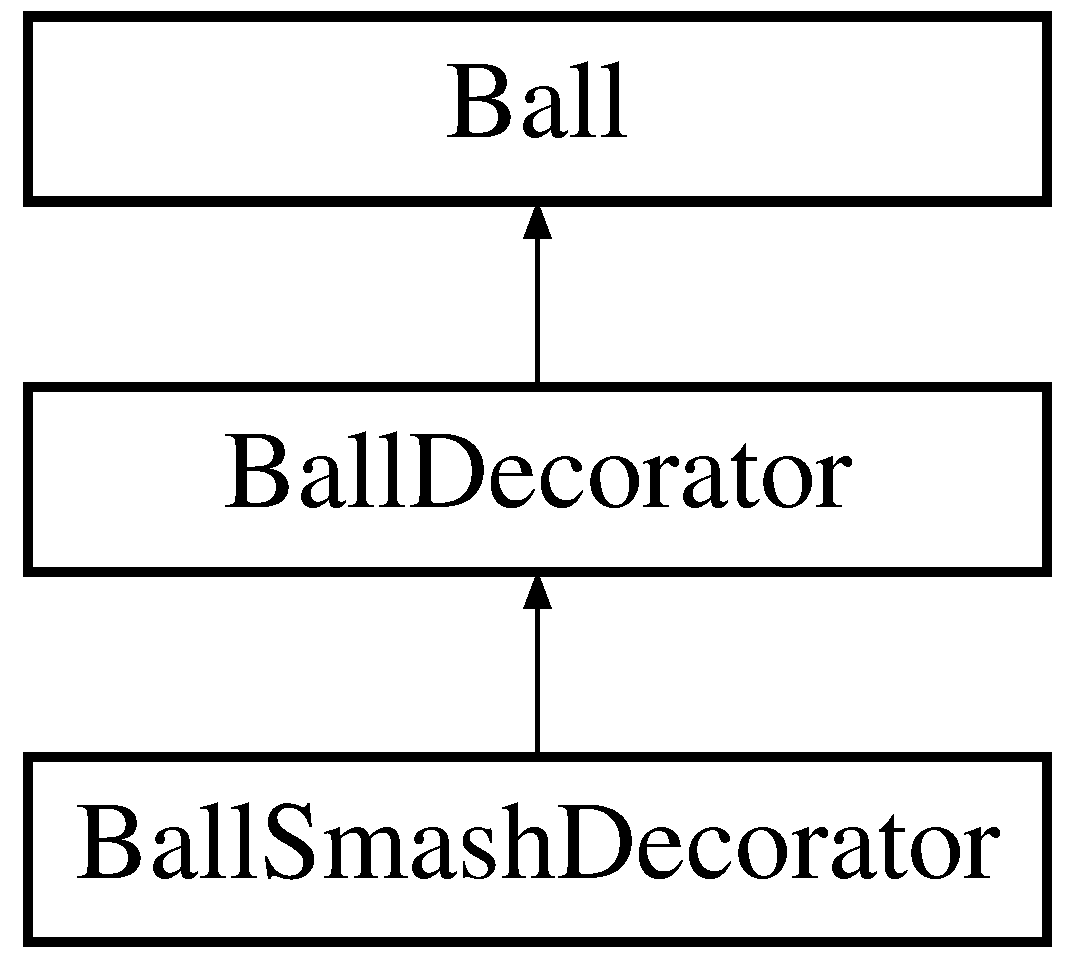
\includegraphics[height=3.000000cm]{class_ball_smash_decorator}
\end{center}
\end{figure}
\subsection*{Classes}
\begin{DoxyCompactItemize}
\item 
struct \mbox{\hyperlink{struct_ball_smash_decorator_1_1_crumb}{Crumb}}
\end{DoxyCompactItemize}
\subsection*{Public Member Functions}
\begin{DoxyCompactItemize}
\item 
\mbox{\hyperlink{class_ball_smash_decorator_a9820f584d49fa51ccf288b6bb4700744}{Ball\+Smash\+Decorator}} (\mbox{\hyperlink{class_ball}{Ball}} $\ast$b)
\item 
virtual void \mbox{\hyperlink{class_ball_smash_decorator_ad59848156e8eabad3e561a1d113f7029}{change\+Velocity}} (const Q\+Vector2D \&delta) override
\begin{DoxyCompactList}\small\item\em change\+Velocity -\/ set the velocity of the ball, as well as generate particles (if applicable) \end{DoxyCompactList}\item 
virtual void \mbox{\hyperlink{class_ball_smash_decorator_a017998926f2b3ebdfcf49e074ea86aae}{multiply\+Velocity}} (const Q\+Vector2D \&vel) override
\begin{DoxyCompactList}\small\item\em multiply\+Velocity -\/ mul the velocity, as well as generate particles, if direction changes. \end{DoxyCompactList}\item 
virtual void \mbox{\hyperlink{class_ball_smash_decorator_a8cbf47d481100f16f2376670fee9fdcc}{render}} (Q\+Painter \&painter, const Q\+Vector2D \&offset) override
\begin{DoxyCompactList}\small\item\em render -\/ draw the ball, the smash particles, as well as update the particle effects positions yes. we animate in the render function! )\+:$<$ \end{DoxyCompactList}\end{DoxyCompactItemize}
\subsection*{Protected Member Functions}
\begin{DoxyCompactItemize}
\item 
void \mbox{\hyperlink{class_ball_smash_decorator_aa800f137e36d43bdfa86843091905186}{add\+Crumbs}} (Q\+PointF c\+Pos)
\end{DoxyCompactItemize}
\subsection*{Protected Attributes}
\begin{DoxyCompactItemize}
\item 
std\+::vector$<$ \mbox{\hyperlink{struct_ball_smash_decorator_1_1_crumb}{Crumb}} $>$ \mbox{\hyperlink{class_ball_smash_decorator_af9860ac78866ac55c8548b7fd8581610}{m\+\_\+crumbs}}
\end{DoxyCompactItemize}
\subsection*{Static Protected Attributes}
\begin{DoxyCompactItemize}
\item 
static constexpr double \mbox{\hyperlink{class_ball_smash_decorator_aeef9438a9102847ca841bc657605e88b}{fade\+Rate}} = 0.\+01
\item 
static constexpr double \mbox{\hyperlink{class_ball_smash_decorator_a947a58aafc3f976931a532974d89abe0}{move\+Rate}} = 0.\+3
\end{DoxyCompactItemize}


\subsection{Detailed Description}


Definition at line 111 of file balldecorator.\+h.



\subsection{Constructor \& Destructor Documentation}
\mbox{\Hypertarget{class_ball_smash_decorator_a9820f584d49fa51ccf288b6bb4700744}\label{class_ball_smash_decorator_a9820f584d49fa51ccf288b6bb4700744}} 
\index{Ball\+Smash\+Decorator@{Ball\+Smash\+Decorator}!Ball\+Smash\+Decorator@{Ball\+Smash\+Decorator}}
\index{Ball\+Smash\+Decorator@{Ball\+Smash\+Decorator}!Ball\+Smash\+Decorator@{Ball\+Smash\+Decorator}}
\subsubsection{\texorpdfstring{Ball\+Smash\+Decorator()}{BallSmashDecorator()}}
{\footnotesize\ttfamily Ball\+Smash\+Decorator\+::\+Ball\+Smash\+Decorator (\begin{DoxyParamCaption}\item[{\mbox{\hyperlink{class_ball}{Ball}} $\ast$}]{b }\end{DoxyParamCaption})\hspace{0.3cm}{\ttfamily [inline]}}



Definition at line 142 of file balldecorator.\+h.



\subsection{Member Function Documentation}
\mbox{\Hypertarget{class_ball_smash_decorator_aa800f137e36d43bdfa86843091905186}\label{class_ball_smash_decorator_aa800f137e36d43bdfa86843091905186}} 
\index{Ball\+Smash\+Decorator@{Ball\+Smash\+Decorator}!add\+Crumbs@{add\+Crumbs}}
\index{add\+Crumbs@{add\+Crumbs}!Ball\+Smash\+Decorator@{Ball\+Smash\+Decorator}}
\subsubsection{\texorpdfstring{add\+Crumbs()}{addCrumbs()}}
{\footnotesize\ttfamily void Ball\+Smash\+Decorator\+::add\+Crumbs (\begin{DoxyParamCaption}\item[{Q\+PointF}]{c\+Pos }\end{DoxyParamCaption})\hspace{0.3cm}{\ttfamily [inline]}, {\ttfamily [protected]}}



Definition at line 132 of file balldecorator.\+h.

\mbox{\Hypertarget{class_ball_smash_decorator_ad59848156e8eabad3e561a1d113f7029}\label{class_ball_smash_decorator_ad59848156e8eabad3e561a1d113f7029}} 
\index{Ball\+Smash\+Decorator@{Ball\+Smash\+Decorator}!change\+Velocity@{change\+Velocity}}
\index{change\+Velocity@{change\+Velocity}!Ball\+Smash\+Decorator@{Ball\+Smash\+Decorator}}
\subsubsection{\texorpdfstring{change\+Velocity()}{changeVelocity()}}
{\footnotesize\ttfamily void Ball\+Smash\+Decorator\+::change\+Velocity (\begin{DoxyParamCaption}\item[{const Q\+Vector2D \&}]{delta }\end{DoxyParamCaption})\hspace{0.3cm}{\ttfamily [override]}, {\ttfamily [virtual]}}



change\+Velocity -\/ set the velocity of the ball, as well as generate particles (if applicable) 


\begin{DoxyParams}{Parameters}
{\em delta} & -\/ the change in velocity \\
\hline
\end{DoxyParams}


Reimplemented from \mbox{\hyperlink{class_ball_decorator_a3e4f4d31f6409f018b8b337bcf2bd284}{Ball\+Decorator}}.



Definition at line 80 of file balldecorator.\+cpp.

\mbox{\Hypertarget{class_ball_smash_decorator_a017998926f2b3ebdfcf49e074ea86aae}\label{class_ball_smash_decorator_a017998926f2b3ebdfcf49e074ea86aae}} 
\index{Ball\+Smash\+Decorator@{Ball\+Smash\+Decorator}!multiply\+Velocity@{multiply\+Velocity}}
\index{multiply\+Velocity@{multiply\+Velocity}!Ball\+Smash\+Decorator@{Ball\+Smash\+Decorator}}
\subsubsection{\texorpdfstring{multiply\+Velocity()}{multiplyVelocity()}}
{\footnotesize\ttfamily virtual void Ball\+Smash\+Decorator\+::multiply\+Velocity (\begin{DoxyParamCaption}\item[{const Q\+Vector2D \&}]{vel }\end{DoxyParamCaption})\hspace{0.3cm}{\ttfamily [inline]}, {\ttfamily [override]}, {\ttfamily [virtual]}}



multiply\+Velocity -\/ mul the velocity, as well as generate particles, if direction changes. 


\begin{DoxyParams}{Parameters}
{\em vel} & \\
\hline
\end{DoxyParams}


Reimplemented from \mbox{\hyperlink{class_ball_decorator_ad1a9139a5c41d17d0eebf007afb984e7}{Ball\+Decorator}}.



Definition at line 154 of file balldecorator.\+h.

\mbox{\Hypertarget{class_ball_smash_decorator_a8cbf47d481100f16f2376670fee9fdcc}\label{class_ball_smash_decorator_a8cbf47d481100f16f2376670fee9fdcc}} 
\index{Ball\+Smash\+Decorator@{Ball\+Smash\+Decorator}!render@{render}}
\index{render@{render}!Ball\+Smash\+Decorator@{Ball\+Smash\+Decorator}}
\subsubsection{\texorpdfstring{render()}{render()}}
{\footnotesize\ttfamily void Ball\+Smash\+Decorator\+::render (\begin{DoxyParamCaption}\item[{Q\+Painter \&}]{painter,  }\item[{const Q\+Vector2D \&}]{offset }\end{DoxyParamCaption})\hspace{0.3cm}{\ttfamily [override]}, {\ttfamily [virtual]}}



render -\/ draw the ball, the smash particles, as well as update the particle effects positions yes. we animate in the render function! )\+:$<$ 


\begin{DoxyParams}{Parameters}
{\em painter} & -\/ the brush to use to draw \\
\hline
{\em offset} & -\/ the offset from the window that this ball\textquotesingle{}s pos is. \\
\hline
\end{DoxyParams}


Reimplemented from \mbox{\hyperlink{class_ball_decorator_af8205f8033b2490ecd3365c24ff5cdeb}{Ball\+Decorator}}.



Definition at line 88 of file balldecorator.\+cpp.



\subsection{Member Data Documentation}
\mbox{\Hypertarget{class_ball_smash_decorator_aeef9438a9102847ca841bc657605e88b}\label{class_ball_smash_decorator_aeef9438a9102847ca841bc657605e88b}} 
\index{Ball\+Smash\+Decorator@{Ball\+Smash\+Decorator}!fade\+Rate@{fade\+Rate}}
\index{fade\+Rate@{fade\+Rate}!Ball\+Smash\+Decorator@{Ball\+Smash\+Decorator}}
\subsubsection{\texorpdfstring{fade\+Rate}{fadeRate}}
{\footnotesize\ttfamily constexpr double Ball\+Smash\+Decorator\+::fade\+Rate = 0.\+01\hspace{0.3cm}{\ttfamily [static]}, {\ttfamily [protected]}}



Definition at line 127 of file balldecorator.\+h.

\mbox{\Hypertarget{class_ball_smash_decorator_af9860ac78866ac55c8548b7fd8581610}\label{class_ball_smash_decorator_af9860ac78866ac55c8548b7fd8581610}} 
\index{Ball\+Smash\+Decorator@{Ball\+Smash\+Decorator}!m\+\_\+crumbs@{m\+\_\+crumbs}}
\index{m\+\_\+crumbs@{m\+\_\+crumbs}!Ball\+Smash\+Decorator@{Ball\+Smash\+Decorator}}
\subsubsection{\texorpdfstring{m\+\_\+crumbs}{m\_crumbs}}
{\footnotesize\ttfamily std\+::vector$<$\mbox{\hyperlink{struct_ball_smash_decorator_1_1_crumb}{Crumb}}$>$ Ball\+Smash\+Decorator\+::m\+\_\+crumbs\hspace{0.3cm}{\ttfamily [protected]}}



Definition at line 130 of file balldecorator.\+h.

\mbox{\Hypertarget{class_ball_smash_decorator_a947a58aafc3f976931a532974d89abe0}\label{class_ball_smash_decorator_a947a58aafc3f976931a532974d89abe0}} 
\index{Ball\+Smash\+Decorator@{Ball\+Smash\+Decorator}!move\+Rate@{move\+Rate}}
\index{move\+Rate@{move\+Rate}!Ball\+Smash\+Decorator@{Ball\+Smash\+Decorator}}
\subsubsection{\texorpdfstring{move\+Rate}{moveRate}}
{\footnotesize\ttfamily constexpr double Ball\+Smash\+Decorator\+::move\+Rate = 0.\+3\hspace{0.3cm}{\ttfamily [static]}, {\ttfamily [protected]}}



Definition at line 129 of file balldecorator.\+h.



The documentation for this class was generated from the following files\+:\begin{DoxyCompactItemize}
\item 
\mbox{\hyperlink{balldecorator_8h}{balldecorator.\+h}}\item 
\mbox{\hyperlink{balldecorator_8cpp}{balldecorator.\+cpp}}\end{DoxyCompactItemize}

\hypertarget{class_ball_sparkle_decorator}{}\section{Ball\+Sparkle\+Decorator Class Reference}
\label{class_ball_sparkle_decorator}\index{Ball\+Sparkle\+Decorator@{Ball\+Sparkle\+Decorator}}


Inherits \mbox{\hyperlink{class_ball_decorator}{Ball\+Decorator}}.

\subsection*{Classes}
\begin{DoxyCompactItemize}
\item 
struct \mbox{\hyperlink{struct_ball_sparkle_decorator_1_1_sparkle}{Sparkle}}
\end{DoxyCompactItemize}
\subsection*{Public Member Functions}
\begin{DoxyCompactItemize}
\item 
\mbox{\Hypertarget{class_ball_sparkle_decorator_aebdaa2c5204a050a297c9255d885d0c3}\label{class_ball_sparkle_decorator_aebdaa2c5204a050a297c9255d885d0c3}} 
{\bfseries Ball\+Sparkle\+Decorator} (\mbox{\hyperlink{class_ball}{Ball}} $\ast$b)
\item 
void \mbox{\hyperlink{class_ball_sparkle_decorator_ad3ee562f1cc9dfa5835bca2fab3d30a7}{render}} (Q\+Painter \&painter, const Q\+Vector2D \&offset) override
\begin{DoxyCompactList}\small\item\em render -\/ draw the underlying ball and also the sparkles \end{DoxyCompactList}\item 
\mbox{\hyperlink{class_ball}{Ball}} $\ast$ \mbox{\hyperlink{class_ball_sparkle_decorator_a1fd1b10d028cc51c958eb5c9a7cf732c}{copy}} () override
\begin{DoxyCompactList}\small\item\em copy it is a deep copy function \end{DoxyCompactList}\end{DoxyCompactItemize}
\subsection*{Protected Attributes}
\begin{DoxyCompactItemize}
\item 
\mbox{\Hypertarget{class_ball_sparkle_decorator_a225c9a37159214fbb658148713227fcf}\label{class_ball_sparkle_decorator_a225c9a37159214fbb658148713227fcf}} 
std\+::vector$<$ \mbox{\hyperlink{struct_ball_sparkle_decorator_1_1_sparkle}{Sparkle}} $>$ {\bfseries m\+\_\+sparkle\+Positions}
\end{DoxyCompactItemize}
\subsection*{Static Protected Attributes}
\begin{DoxyCompactItemize}
\item 
\mbox{\Hypertarget{class_ball_sparkle_decorator_ad4e98ec20a12be0c8b0481879d4c2d17}\label{class_ball_sparkle_decorator_ad4e98ec20a12be0c8b0481879d4c2d17}} 
static constexpr double {\bfseries fade\+Rate} = 0.\+01
\end{DoxyCompactItemize}


\subsection{Member Function Documentation}
\mbox{\Hypertarget{class_ball_sparkle_decorator_a1fd1b10d028cc51c958eb5c9a7cf732c}\label{class_ball_sparkle_decorator_a1fd1b10d028cc51c958eb5c9a7cf732c}} 
\index{Ball\+Sparkle\+Decorator@{Ball\+Sparkle\+Decorator}!copy@{copy}}
\index{copy@{copy}!Ball\+Sparkle\+Decorator@{Ball\+Sparkle\+Decorator}}
\subsubsection{\texorpdfstring{copy()}{copy()}}
{\footnotesize\ttfamily \mbox{\hyperlink{class_ball}{Ball}} $\ast$ Ball\+Sparkle\+Decorator\+::copy (\begin{DoxyParamCaption}{ }\end{DoxyParamCaption})\hspace{0.3cm}{\ttfamily [override]}, {\ttfamily [virtual]}}



copy it is a deep copy function 

\begin{DoxyReturn}{Returns}
A new ball with different address 
\end{DoxyReturn}


Implements \mbox{\hyperlink{class_ball_ae6c0731fabb7a45ba36df62a1975661a}{Ball}}.

\mbox{\Hypertarget{class_ball_sparkle_decorator_ad3ee562f1cc9dfa5835bca2fab3d30a7}\label{class_ball_sparkle_decorator_ad3ee562f1cc9dfa5835bca2fab3d30a7}} 
\index{Ball\+Sparkle\+Decorator@{Ball\+Sparkle\+Decorator}!render@{render}}
\index{render@{render}!Ball\+Sparkle\+Decorator@{Ball\+Sparkle\+Decorator}}
\subsubsection{\texorpdfstring{render()}{render()}}
{\footnotesize\ttfamily void Ball\+Sparkle\+Decorator\+::render (\begin{DoxyParamCaption}\item[{Q\+Painter \&}]{painter,  }\item[{const Q\+Vector2D \&}]{offset }\end{DoxyParamCaption})\hspace{0.3cm}{\ttfamily [override]}, {\ttfamily [virtual]}}



render -\/ draw the underlying ball and also the sparkles 


\begin{DoxyParams}{Parameters}
{\em painter} & -\/ the brush to use to draw \\
\hline
{\em offset} & -\/ the offset that this ball is from the origin \\
\hline
\end{DoxyParams}


Reimplemented from \mbox{\hyperlink{class_ball_decorator_af8205f8033b2490ecd3365c24ff5cdeb}{Ball\+Decorator}}.



The documentation for this class was generated from the following files\+:\begin{DoxyCompactItemize}
\item 
balldecorator.\+h\item 
balldecorator.\+cpp\end{DoxyCompactItemize}

\hypertarget{class_composite_ball}{}\section{Composite\+Ball Class Reference}
\label{class_composite_ball}\index{Composite\+Ball@{Composite\+Ball}}


{\ttfamily \#include $<$ball.\+h$>$}

Inheritance diagram for Composite\+Ball\+:\begin{figure}[H]
\begin{center}
\leavevmode
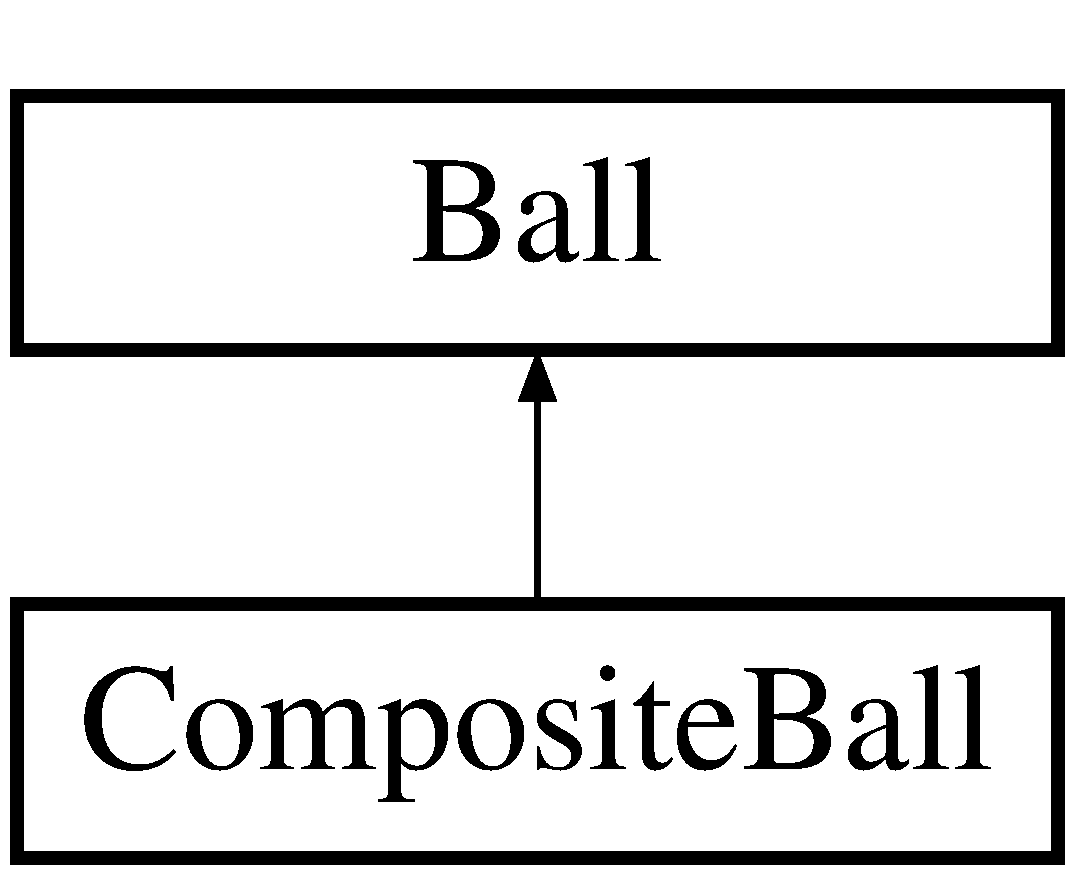
\includegraphics[height=2.000000cm]{class_composite_ball}
\end{center}
\end{figure}
\subsection*{Public Member Functions}
\begin{DoxyCompactItemize}
\item 
\mbox{\hyperlink{class_composite_ball_a7b6224c07ad69240377555508ddc8876}{Composite\+Ball}} (Q\+Color colour, Q\+Vector2D position, Q\+Vector2D velocity, double mass, int radius, double strength)
\item 
void \mbox{\hyperlink{class_composite_ball_a2aefe32771e1cde5dc8f51d779c880eb}{render}} (Q\+Painter \&painter, const Q\+Vector2D \&offset) override
\begin{DoxyCompactList}\small\item\em render -\/ draw the ball to the screen \end{DoxyCompactList}\item 
void \mbox{\hyperlink{class_composite_ball_a6c226ee364012b0c3eb3271a01307297}{add\+Child}} (\mbox{\hyperlink{class_ball}{Ball}} $\ast$b)
\item 
virtual bool \mbox{\hyperlink{class_composite_ball_a0da2c5749caafcef943f14a500a0fc9b}{apply\+Break}} (const Q\+Vector2D \&deltaV, std\+::vector$<$ \mbox{\hyperlink{class_ball}{Ball}} $\ast$$>$ \&parentlist) override
\begin{DoxyCompactList}\small\item\em apply\+Break -\/ check and resolve breaking balls \end{DoxyCompactList}\end{DoxyCompactItemize}
\subsection*{Protected Member Functions}
\begin{DoxyCompactItemize}
\item 
void \mbox{\hyperlink{class_composite_ball_a05f96cd1c4321d89763dce5a15b53138}{recursive\+Render}} (Q\+Painter \&painter, const Q\+Vector2D \&offset)
\end{DoxyCompactItemize}
\subsection*{Protected Attributes}
\begin{DoxyCompactItemize}
\item 
std\+::vector$<$ \mbox{\hyperlink{class_ball}{Ball}} $\ast$ $>$ \mbox{\hyperlink{class_composite_ball_a2689ad5361a52d586f43dafd8922a422}{m\+\_\+children}}
\item 
bool \mbox{\hyperlink{class_composite_ball_a751e10b0f9278bcf48720ac6af9bdd20}{m\+\_\+render\+Children}} = true
\item 
double \mbox{\hyperlink{class_composite_ball_a78051a7a01a600b88ed22e7d725640db}{m\+\_\+strength}} = std\+::numeric\+\_\+limits$<$double$>$\+::max()
\end{DoxyCompactItemize}
\subsection*{Additional Inherited Members}


\subsection{Detailed Description}


Definition at line 72 of file ball.\+h.



\subsection{Constructor \& Destructor Documentation}
\mbox{\Hypertarget{class_composite_ball_a7b6224c07ad69240377555508ddc8876}\label{class_composite_ball_a7b6224c07ad69240377555508ddc8876}} 
\index{Composite\+Ball@{Composite\+Ball}!Composite\+Ball@{Composite\+Ball}}
\index{Composite\+Ball@{Composite\+Ball}!Composite\+Ball@{Composite\+Ball}}
\subsubsection{\texorpdfstring{Composite\+Ball()}{CompositeBall()}}
{\footnotesize\ttfamily Composite\+Ball\+::\+Composite\+Ball (\begin{DoxyParamCaption}\item[{Q\+Color}]{colour,  }\item[{Q\+Vector2D}]{position,  }\item[{Q\+Vector2D}]{velocity,  }\item[{double}]{mass,  }\item[{int}]{radius,  }\item[{double}]{strength }\end{DoxyParamCaption})\hspace{0.3cm}{\ttfamily [inline]}}



Definition at line 80 of file ball.\+h.



\subsection{Member Function Documentation}
\mbox{\Hypertarget{class_composite_ball_a6c226ee364012b0c3eb3271a01307297}\label{class_composite_ball_a6c226ee364012b0c3eb3271a01307297}} 
\index{Composite\+Ball@{Composite\+Ball}!add\+Child@{add\+Child}}
\index{add\+Child@{add\+Child}!Composite\+Ball@{Composite\+Ball}}
\subsubsection{\texorpdfstring{add\+Child()}{addChild()}}
{\footnotesize\ttfamily void Composite\+Ball\+::add\+Child (\begin{DoxyParamCaption}\item[{\mbox{\hyperlink{class_ball}{Ball}} $\ast$}]{b }\end{DoxyParamCaption})\hspace{0.3cm}{\ttfamily [inline]}}



Definition at line 91 of file ball.\+h.

\mbox{\Hypertarget{class_composite_ball_a0da2c5749caafcef943f14a500a0fc9b}\label{class_composite_ball_a0da2c5749caafcef943f14a500a0fc9b}} 
\index{Composite\+Ball@{Composite\+Ball}!apply\+Break@{apply\+Break}}
\index{apply\+Break@{apply\+Break}!Composite\+Ball@{Composite\+Ball}}
\subsubsection{\texorpdfstring{apply\+Break()}{applyBreak()}}
{\footnotesize\ttfamily bool Composite\+Ball\+::apply\+Break (\begin{DoxyParamCaption}\item[{const Q\+Vector2D \&}]{deltaV,  }\item[{std\+::vector$<$ \mbox{\hyperlink{class_ball}{Ball}} $\ast$$>$ \&}]{parentlist }\end{DoxyParamCaption})\hspace{0.3cm}{\ttfamily [override]}, {\ttfamily [virtual]}}



apply\+Break -\/ check and resolve breaking balls 


\begin{DoxyParams}{Parameters}
{\em deltaV} & -\/ the change in velocity \\
\hline
{\em parentlist} & -\/ the list of balls that we\textquotesingle{}ll need to add to if we break anything \\
\hline
\end{DoxyParams}
\begin{DoxyReturn}{Returns}
whether the ball broke or not 
\end{DoxyReturn}


Reimplemented from \mbox{\hyperlink{class_ball_a9df4c9fc8620d003cf9717d84e64d5ee}{Ball}}.



Definition at line 26 of file ball.\+cpp.

\mbox{\Hypertarget{class_composite_ball_a05f96cd1c4321d89763dce5a15b53138}\label{class_composite_ball_a05f96cd1c4321d89763dce5a15b53138}} 
\index{Composite\+Ball@{Composite\+Ball}!recursive\+Render@{recursive\+Render}}
\index{recursive\+Render@{recursive\+Render}!Composite\+Ball@{Composite\+Ball}}
\subsubsection{\texorpdfstring{recursive\+Render()}{recursiveRender()}}
{\footnotesize\ttfamily void Composite\+Ball\+::recursive\+Render (\begin{DoxyParamCaption}\item[{Q\+Painter \&}]{painter,  }\item[{const Q\+Vector2D \&}]{offset }\end{DoxyParamCaption})\hspace{0.3cm}{\ttfamily [protected]}}



Definition at line 15 of file ball.\+cpp.

\mbox{\Hypertarget{class_composite_ball_a2aefe32771e1cde5dc8f51d779c880eb}\label{class_composite_ball_a2aefe32771e1cde5dc8f51d779c880eb}} 
\index{Composite\+Ball@{Composite\+Ball}!render@{render}}
\index{render@{render}!Composite\+Ball@{Composite\+Ball}}
\subsubsection{\texorpdfstring{render()}{render()}}
{\footnotesize\ttfamily void Composite\+Ball\+::render (\begin{DoxyParamCaption}\item[{Q\+Painter \&}]{painter,  }\item[{const Q\+Vector2D \&}]{offset }\end{DoxyParamCaption})\hspace{0.3cm}{\ttfamily [override]}, {\ttfamily [virtual]}}



render -\/ draw the ball to the screen 


\begin{DoxyParams}{Parameters}
{\em painter} & -\/ Q\+Painter that is owned by the dialog \\
\hline
\end{DoxyParams}


Implements \mbox{\hyperlink{class_ball_a307773aaa59aee90cef8767b0c22deca}{Ball}}.



Definition at line 11 of file ball.\+cpp.



\subsection{Member Data Documentation}
\mbox{\Hypertarget{class_composite_ball_a2689ad5361a52d586f43dafd8922a422}\label{class_composite_ball_a2689ad5361a52d586f43dafd8922a422}} 
\index{Composite\+Ball@{Composite\+Ball}!m\+\_\+children@{m\+\_\+children}}
\index{m\+\_\+children@{m\+\_\+children}!Composite\+Ball@{Composite\+Ball}}
\subsubsection{\texorpdfstring{m\+\_\+children}{m\_children}}
{\footnotesize\ttfamily std\+::vector$<$\mbox{\hyperlink{class_ball}{Ball}}$\ast$$>$ Composite\+Ball\+::m\+\_\+children\hspace{0.3cm}{\ttfamily [protected]}}



Definition at line 74 of file ball.\+h.

\mbox{\Hypertarget{class_composite_ball_a751e10b0f9278bcf48720ac6af9bdd20}\label{class_composite_ball_a751e10b0f9278bcf48720ac6af9bdd20}} 
\index{Composite\+Ball@{Composite\+Ball}!m\+\_\+render\+Children@{m\+\_\+render\+Children}}
\index{m\+\_\+render\+Children@{m\+\_\+render\+Children}!Composite\+Ball@{Composite\+Ball}}
\subsubsection{\texorpdfstring{m\+\_\+render\+Children}{m\_renderChildren}}
{\footnotesize\ttfamily bool Composite\+Ball\+::m\+\_\+render\+Children = true\hspace{0.3cm}{\ttfamily [protected]}}



Definition at line 75 of file ball.\+h.

\mbox{\Hypertarget{class_composite_ball_a78051a7a01a600b88ed22e7d725640db}\label{class_composite_ball_a78051a7a01a600b88ed22e7d725640db}} 
\index{Composite\+Ball@{Composite\+Ball}!m\+\_\+strength@{m\+\_\+strength}}
\index{m\+\_\+strength@{m\+\_\+strength}!Composite\+Ball@{Composite\+Ball}}
\subsubsection{\texorpdfstring{m\+\_\+strength}{m\_strength}}
{\footnotesize\ttfamily double Composite\+Ball\+::m\+\_\+strength = std\+::numeric\+\_\+limits$<$double$>$\+::max()\hspace{0.3cm}{\ttfamily [protected]}}



Definition at line 78 of file ball.\+h.



The documentation for this class was generated from the following files\+:\begin{DoxyCompactItemize}
\item 
\mbox{\hyperlink{ball_8h}{ball.\+h}}\item 
\mbox{\hyperlink{ball_8cpp}{ball.\+cpp}}\end{DoxyCompactItemize}

\hypertarget{struct_ball_smash_decorator_1_1_crumb}{}\section{Ball\+Smash\+Decorator\+:\+:Crumb Struct Reference}
\label{struct_ball_smash_decorator_1_1_crumb}\index{Ball\+Smash\+Decorator\+::\+Crumb@{Ball\+Smash\+Decorator\+::\+Crumb}}
\subsection*{Public Member Functions}
\begin{DoxyCompactItemize}
\item 
\mbox{\Hypertarget{struct_ball_smash_decorator_1_1_crumb_a56aecb399208100c5949fd769841c471}\label{struct_ball_smash_decorator_1_1_crumb_a56aecb399208100c5949fd769841c471}} 
{\bfseries Crumb} (Q\+PointF pos, double width, double height, Q\+Vector2D dir, double opacity=1.\+0)
\end{DoxyCompactItemize}
\subsection*{Public Attributes}
\begin{DoxyCompactItemize}
\item 
\mbox{\Hypertarget{struct_ball_smash_decorator_1_1_crumb_a227020594ba8919c73e6d99b81295015}\label{struct_ball_smash_decorator_1_1_crumb_a227020594ba8919c73e6d99b81295015}} 
Q\+PointF {\bfseries pos}
\item 
\mbox{\Hypertarget{struct_ball_smash_decorator_1_1_crumb_a819ee5d8334f427a3e88d50dd020ff41}\label{struct_ball_smash_decorator_1_1_crumb_a819ee5d8334f427a3e88d50dd020ff41}} 
double {\bfseries width} = 5.\+0
\item 
\mbox{\Hypertarget{struct_ball_smash_decorator_1_1_crumb_a127266575a109f1074ef8d007abcf97d}\label{struct_ball_smash_decorator_1_1_crumb_a127266575a109f1074ef8d007abcf97d}} 
double {\bfseries height} = 5.\+0
\item 
\mbox{\Hypertarget{struct_ball_smash_decorator_1_1_crumb_aae0338b32f39f2afafdc80796591fe24}\label{struct_ball_smash_decorator_1_1_crumb_aae0338b32f39f2afafdc80796591fe24}} 
Q\+Vector2D {\bfseries dir}
\item 
\mbox{\Hypertarget{struct_ball_smash_decorator_1_1_crumb_a7d3c5a6ae93d33b50fc6209e2573ac80}\label{struct_ball_smash_decorator_1_1_crumb_a7d3c5a6ae93d33b50fc6209e2573ac80}} 
double {\bfseries opacity} = 1.\+0
\end{DoxyCompactItemize}


The documentation for this struct was generated from the following file\+:\begin{DoxyCompactItemize}
\item 
balldecorator.\+h\end{DoxyCompactItemize}

\hypertarget{class_cue_ball}{}\section{Cue\+Ball Class Reference}
\label{class_cue_ball}\index{Cue\+Ball@{Cue\+Ball}}


The \mbox{\hyperlink{class_cue_ball}{Cue\+Ball}} class This handles some mouse interactions, and can control the position/velocity of the ball The ball will only be able to be controlled if the mouse click\&drag event originated at the position of the cue ball.  




{\ttfamily \#include $<$balldecorator.\+h$>$}



Inherits \mbox{\hyperlink{class_ball_decorator}{Ball\+Decorator}}.

\subsection*{Public Member Functions}
\begin{DoxyCompactItemize}
\item 
\mbox{\Hypertarget{class_cue_ball_a9a5dd540283fcd724b7f1a3bce11fbf0}\label{class_cue_ball_a9a5dd540283fcd724b7f1a3bce11fbf0}} 
{\bfseries Cue\+Ball} (\mbox{\hyperlink{class_ball}{Ball}} $\ast$b)
\item 
void \mbox{\hyperlink{class_cue_ball_a915a83205e4cfc720fbd884b045e2f81}{render}} (Q\+Painter \&painter, const Q\+Vector2D \&offset) override
\begin{DoxyCompactList}\small\item\em render -\/ draw this ball and the drag indicator if applicable \end{DoxyCompactList}\item 
void \mbox{\hyperlink{class_cue_ball_aa6165c3e37540234b621402e02c1c97c}{set\+Start\+Mouse\+Pos}} (Q\+Vector2D p)
\begin{DoxyCompactList}\small\item\em set\+Start\+Mouse\+Pos -\/ update where the start of the mouse drag is. Chooses not to draw IF the click is not within bounds \end{DoxyCompactList}\item 
void \mbox{\hyperlink{class_cue_ball_a297112b81595f308f717410f74d03d3c}{set\+End\+Mouse\+Pos}} (Q\+Vector2D p)
\begin{DoxyCompactList}\small\item\em set\+End\+Mouse\+Pos -\/ update where the current end of the mouse drag is. Used when the mouse is moved, i.\+e. not released, but dragged. \end{DoxyCompactList}\item 
void \mbox{\hyperlink{class_cue_ball_a8aafe19b8226adfcca93621baeef29f4}{set\+Release\+Pos}} (Q\+Vector2D p)
\begin{DoxyCompactList}\small\item\em set\+Release\+Pos -\/ update where the end of the mouse drag is, \& release the click This will update the ball velocity if drawn. \end{DoxyCompactList}\item 
void \mbox{\hyperlink{class_cue_ball_aaab036efaf9d498af1a70cf3e68db11e}{set\+Is\+Hitting}} (bool state)
\begin{DoxyCompactList}\small\item\em set\+Is\+Hitting -\/ update where the stick is hitting the ball This will allow the time to drawing the stick. \end{DoxyCompactList}\item 
\mbox{\Hypertarget{class_cue_ball_a7035345f6ba5c29052a5a1444e3f076f}\label{class_cue_ball_a7035345f6ba5c29052a5a1444e3f076f}} 
bool {\bfseries is\+Sub\+Ball\+Moving} () const
\item 
\mbox{\hyperlink{class_ball}{Ball}} $\ast$ \mbox{\hyperlink{class_cue_ball_a9c2d69ffe6892cba695ef34e360b5dae}{copy}} () override
\begin{DoxyCompactList}\small\item\em copy it is a deep copy function \end{DoxyCompactList}\end{DoxyCompactItemize}
\subsection*{Protected Attributes}
\begin{DoxyCompactItemize}
\item 
\mbox{\Hypertarget{class_cue_ball_a31c90da6dfe1fcaba9dae9a9860028b9}\label{class_cue_ball_a31c90da6dfe1fcaba9dae9a9860028b9}} 
Q\+Vector2D {\bfseries m\+\_\+start\+Mouse\+Pos}
\item 
\mbox{\Hypertarget{class_cue_ball_a2266dea32739c919dbd7848167536a4e}\label{class_cue_ball_a2266dea32739c919dbd7848167536a4e}} 
Q\+Vector2D {\bfseries m\+\_\+end\+Mouse\+Pos}
\item 
\mbox{\Hypertarget{class_cue_ball_a83f8528e08491dc39f22888ddd3bfdff}\label{class_cue_ball_a83f8528e08491dc39f22888ddd3bfdff}} 
bool {\bfseries is\+Drawing} = false
\item 
\mbox{\Hypertarget{class_cue_ball_ade31163403f593728955ee17d7bfa52e}\label{class_cue_ball_ade31163403f593728955ee17d7bfa52e}} 
bool {\bfseries is\+Hitting} = false
\item 
\mbox{\Hypertarget{class_cue_ball_a7d96d4cd6ddda11c9be9ef7c6de36701}\label{class_cue_ball_a7d96d4cd6ddda11c9be9ef7c6de36701}} 
int {\bfseries hitting\+\_\+count} = 8
\item 
\mbox{\Hypertarget{class_cue_ball_a8c9e20f373e0fdb320f2caf482667091}\label{class_cue_ball_a8c9e20f373e0fdb320f2caf482667091}} 
Q\+Vector2D {\bfseries resulting\+Vel}
\end{DoxyCompactItemize}
\subsection*{Additional Inherited Members}


\subsection{Detailed Description}
The \mbox{\hyperlink{class_cue_ball}{Cue\+Ball}} class This handles some mouse interactions, and can control the position/velocity of the ball The ball will only be able to be controlled if the mouse click\&drag event originated at the position of the cue ball. 

\subsection{Member Function Documentation}
\mbox{\Hypertarget{class_cue_ball_a9c2d69ffe6892cba695ef34e360b5dae}\label{class_cue_ball_a9c2d69ffe6892cba695ef34e360b5dae}} 
\index{Cue\+Ball@{Cue\+Ball}!copy@{copy}}
\index{copy@{copy}!Cue\+Ball@{Cue\+Ball}}
\subsubsection{\texorpdfstring{copy()}{copy()}}
{\footnotesize\ttfamily \mbox{\hyperlink{class_ball}{Ball}} $\ast$ Cue\+Ball\+::copy (\begin{DoxyParamCaption}{ }\end{DoxyParamCaption})\hspace{0.3cm}{\ttfamily [override]}, {\ttfamily [virtual]}}



copy it is a deep copy function 

\begin{DoxyReturn}{Returns}
A new ball with different address 
\end{DoxyReturn}


Implements \mbox{\hyperlink{class_ball_ae6c0731fabb7a45ba36df62a1975661a}{Ball}}.

\mbox{\Hypertarget{class_cue_ball_a915a83205e4cfc720fbd884b045e2f81}\label{class_cue_ball_a915a83205e4cfc720fbd884b045e2f81}} 
\index{Cue\+Ball@{Cue\+Ball}!render@{render}}
\index{render@{render}!Cue\+Ball@{Cue\+Ball}}
\subsubsection{\texorpdfstring{render()}{render()}}
{\footnotesize\ttfamily void Cue\+Ball\+::render (\begin{DoxyParamCaption}\item[{Q\+Painter \&}]{painter,  }\item[{const Q\+Vector2D \&}]{offset }\end{DoxyParamCaption})\hspace{0.3cm}{\ttfamily [override]}, {\ttfamily [virtual]}}



render -\/ draw this ball and the drag indicator if applicable 


\begin{DoxyParams}{Parameters}
{\em painter} & -\/ the brush to use to draw \\
\hline
{\em offset} & -\/ where our pos is relative to \\
\hline
\end{DoxyParams}


Reimplemented from \mbox{\hyperlink{class_ball_decorator_af8205f8033b2490ecd3365c24ff5cdeb}{Ball\+Decorator}}.

\mbox{\Hypertarget{class_cue_ball_a297112b81595f308f717410f74d03d3c}\label{class_cue_ball_a297112b81595f308f717410f74d03d3c}} 
\index{Cue\+Ball@{Cue\+Ball}!set\+End\+Mouse\+Pos@{set\+End\+Mouse\+Pos}}
\index{set\+End\+Mouse\+Pos@{set\+End\+Mouse\+Pos}!Cue\+Ball@{Cue\+Ball}}
\subsubsection{\texorpdfstring{set\+End\+Mouse\+Pos()}{setEndMousePos()}}
{\footnotesize\ttfamily void Cue\+Ball\+::set\+End\+Mouse\+Pos (\begin{DoxyParamCaption}\item[{Q\+Vector2D}]{p }\end{DoxyParamCaption})}



set\+End\+Mouse\+Pos -\/ update where the current end of the mouse drag is. Used when the mouse is moved, i.\+e. not released, but dragged. 


\begin{DoxyParams}{Parameters}
{\em p} & \\
\hline
\end{DoxyParams}
\mbox{\Hypertarget{class_cue_ball_aaab036efaf9d498af1a70cf3e68db11e}\label{class_cue_ball_aaab036efaf9d498af1a70cf3e68db11e}} 
\index{Cue\+Ball@{Cue\+Ball}!set\+Is\+Hitting@{set\+Is\+Hitting}}
\index{set\+Is\+Hitting@{set\+Is\+Hitting}!Cue\+Ball@{Cue\+Ball}}
\subsubsection{\texorpdfstring{set\+Is\+Hitting()}{setIsHitting()}}
{\footnotesize\ttfamily void Cue\+Ball\+::set\+Is\+Hitting (\begin{DoxyParamCaption}\item[{bool}]{state }\end{DoxyParamCaption})\hspace{0.3cm}{\ttfamily [inline]}}



set\+Is\+Hitting -\/ update where the stick is hitting the ball This will allow the time to drawing the stick. 


\begin{DoxyParams}{Parameters}
{\em state} & \\
\hline
\end{DoxyParams}
\mbox{\Hypertarget{class_cue_ball_a8aafe19b8226adfcca93621baeef29f4}\label{class_cue_ball_a8aafe19b8226adfcca93621baeef29f4}} 
\index{Cue\+Ball@{Cue\+Ball}!set\+Release\+Pos@{set\+Release\+Pos}}
\index{set\+Release\+Pos@{set\+Release\+Pos}!Cue\+Ball@{Cue\+Ball}}
\subsubsection{\texorpdfstring{set\+Release\+Pos()}{setReleasePos()}}
{\footnotesize\ttfamily void Cue\+Ball\+::set\+Release\+Pos (\begin{DoxyParamCaption}\item[{Q\+Vector2D}]{p }\end{DoxyParamCaption})}



set\+Release\+Pos -\/ update where the end of the mouse drag is, \& release the click This will update the ball velocity if drawn. 


\begin{DoxyParams}{Parameters}
{\em p} & \\
\hline
\end{DoxyParams}
\mbox{\Hypertarget{class_cue_ball_aa6165c3e37540234b621402e02c1c97c}\label{class_cue_ball_aa6165c3e37540234b621402e02c1c97c}} 
\index{Cue\+Ball@{Cue\+Ball}!set\+Start\+Mouse\+Pos@{set\+Start\+Mouse\+Pos}}
\index{set\+Start\+Mouse\+Pos@{set\+Start\+Mouse\+Pos}!Cue\+Ball@{Cue\+Ball}}
\subsubsection{\texorpdfstring{set\+Start\+Mouse\+Pos()}{setStartMousePos()}}
{\footnotesize\ttfamily void Cue\+Ball\+::set\+Start\+Mouse\+Pos (\begin{DoxyParamCaption}\item[{Q\+Vector2D}]{p }\end{DoxyParamCaption})}



set\+Start\+Mouse\+Pos -\/ update where the start of the mouse drag is. Chooses not to draw IF the click is not within bounds 


\begin{DoxyParams}{Parameters}
{\em p} & -\/ the mouse click pos, relative to the Q\+Widget \\
\hline
\end{DoxyParams}


The documentation for this class was generated from the following files\+:\begin{DoxyCompactItemize}
\item 
balldecorator.\+h\item 
balldecorator.\+cpp\end{DoxyCompactItemize}

\hypertarget{class_dialog}{}\section{Dialog Class Reference}
\label{class_dialog}\index{Dialog@{Dialog}}


Inherits Q\+Dialog.

\subsection*{Public Slots}
\begin{DoxyCompactItemize}
\item 
\mbox{\Hypertarget{class_dialog_a45158754d3f4531b29a0f50abde94597}\label{class_dialog_a45158754d3f4531b29a0f50abde94597}} 
void \mbox{\hyperlink{class_dialog_a45158754d3f4531b29a0f50abde94597}{next\+Anim}} ()
\begin{DoxyCompactList}\small\item\em next\+Anim -\/ move the objects and perform collision events \end{DoxyCompactList}\item 
\mbox{\Hypertarget{class_dialog_aa887f720e12758049bb9f1f1814759da}\label{class_dialog_aa887f720e12758049bb9f1f1814759da}} 
void \mbox{\hyperlink{class_dialog_aa887f720e12758049bb9f1f1814759da}{try\+Render}} ()
\begin{DoxyCompactList}\small\item\em try\+Render -\/ draw the objects to screen \end{DoxyCompactList}\item 
\mbox{\Hypertarget{class_dialog_a193bf90e041064df1a5c7f40d251734a}\label{class_dialog_a193bf90e041064df1a5c7f40d251734a}} 
void {\bfseries handle\+Add\+Button} ()
\item 
\mbox{\Hypertarget{class_dialog_aed18452251b1a5f073e552d346f6398f}\label{class_dialog_aed18452251b1a5f073e552d346f6398f}} 
void {\bfseries handle\+Replace\+Button} ()
\item 
\mbox{\Hypertarget{class_dialog_a95aaa4d78bda5c07650d383d3c5292ac}\label{class_dialog_a95aaa4d78bda5c07650d383d3c5292ac}} 
void {\bfseries mouse\+Press\+Event} (Q\+Mouse\+Event $\ast$event)
\item 
\mbox{\Hypertarget{class_dialog_a95158bddb719a98816c8432ddb096b27}\label{class_dialog_a95158bddb719a98816c8432ddb096b27}} 
void {\bfseries mouse\+Release\+Event} (Q\+Mouse\+Event $\ast$event)
\item 
\mbox{\Hypertarget{class_dialog_aea6bb029efbb1eaa374bd938ff0afabf}\label{class_dialog_aea6bb029efbb1eaa374bd938ff0afabf}} 
void {\bfseries mouse\+Move\+Event} (Q\+Mouse\+Event $\ast$event)
\item 
\mbox{\Hypertarget{class_dialog_aa687205f957253ec53f4ce47b49d302b}\label{class_dialog_aa687205f957253ec53f4ce47b49d302b}} 
void {\bfseries key\+Press\+Event} (Q\+Key\+Event $\ast$event)
\end{DoxyCompactItemize}
\subsection*{Public Member Functions}
\begin{DoxyCompactItemize}
\item 
\mbox{\Hypertarget{class_dialog_a50ae9716ee548a6f31fc5d0a29347899}\label{class_dialog_a50ae9716ee548a6f31fc5d0a29347899}} 
{\bfseries Dialog} (\mbox{\hyperlink{class_game}{Game}} $\ast$game, Q\+Widget $\ast$parent=0)
\end{DoxyCompactItemize}
\subsection*{Protected Member Functions}
\begin{DoxyCompactItemize}
\item 
\mbox{\Hypertarget{class_dialog_a93e4c843803f26bfe5746529cf163ec5}\label{class_dialog_a93e4c843803f26bfe5746529cf163ec5}} 
void \mbox{\hyperlink{class_dialog_a93e4c843803f26bfe5746529cf163ec5}{paint\+Event}} (Q\+Paint\+Event $\ast$)
\begin{DoxyCompactList}\small\item\em paint\+Event -\/ called whenever window repainting is requested \end{DoxyCompactList}\end{DoxyCompactItemize}


The documentation for this class was generated from the following files\+:\begin{DoxyCompactItemize}
\item 
dialog.\+h\item 
dialog.\+cpp\end{DoxyCompactItemize}

\hypertarget{class_game}{}\section{Game Class Reference}
\label{class_game}\index{Game@{Game}}


{\ttfamily \#include $<$game.\+h$>$}

\subsection*{Public Member Functions}
\begin{DoxyCompactItemize}
\item 
\mbox{\hyperlink{class_game_ae3d112ca6e0e55150d2fdbc704474530}{$\sim$\+Game}} ()
\item 
\mbox{\hyperlink{class_game_a1d3aba143e23c5b7bafda7852c2ce3b9}{Game}} (std\+::vector$<$ \mbox{\hyperlink{class_ball}{Ball}} $\ast$$>$ $\ast$balls, \mbox{\hyperlink{class_table}{Table}} $\ast$table)
\item 
void \mbox{\hyperlink{class_game_af80284dbc78f4829aeb0f2420373f605}{render}} (Q\+Painter \&painter) const
\begin{DoxyCompactList}\small\item\em Draws all owned objects to the screen (balls and table) \end{DoxyCompactList}\item 
void \mbox{\hyperlink{class_game_a40c08e2135ae529a820cdeeff32c5144}{animate}} (double dt)
\begin{DoxyCompactList}\small\item\em Updates the positions of all objects within, based on how much time has changed. \end{DoxyCompactList}\item 
int \mbox{\hyperlink{class_game_a0eee5d6dca8985da6e57bd548214a507}{get\+Minimum\+Width}} () const
\item 
int \mbox{\hyperlink{class_game_a0712183d4b571d7e3aeb60745b597abd}{get\+Minimum\+Height}} () const
\item 
Q\+Vector2D \mbox{\hyperlink{class_game_a8063ed6374c6bbadad0cbe71364fe764}{resolve\+Collision}} (const \mbox{\hyperlink{class_table}{Table}} $\ast$table, \mbox{\hyperlink{class_ball}{Ball}} $\ast$ball)
\begin{DoxyCompactList}\small\item\em resolve\+Collision -\/ modify the ball\textquotesingle{}s velocity if it is colliding with the table \end{DoxyCompactList}\item 
std\+::pair$<$ Q\+Vector2D, Q\+Vector2D $>$ \mbox{\hyperlink{class_game_ac7de6f8d4a2131befbf6dbcccb6921f1}{resolve\+Collision}} (\mbox{\hyperlink{class_ball}{Ball}} $\ast$ballA, \mbox{\hyperlink{class_ball}{Ball}} $\ast$ballB)
\begin{DoxyCompactList}\small\item\em resolve\+Collision -\/ resolve both ball\textquotesingle{}s velocity whether these balls collide \end{DoxyCompactList}\item 
bool \mbox{\hyperlink{class_game_ac574803a4cd9cb5f52f72268c5f22b40}{is\+Colliding}} (const \mbox{\hyperlink{class_ball}{Ball}} $\ast$ballA, const \mbox{\hyperlink{class_ball}{Ball}} $\ast$ballB)
\begin{DoxyCompactList}\small\item\em is\+Colliding -\/ returns whether two balls are touching each other \end{DoxyCompactList}\item 
void \mbox{\hyperlink{class_game_a14d2f562cd2e237844c8c3af5ed3bc21}{set\+Start\+Mouse\+Pos}} (Q\+Vector2D p)
\item 
void \mbox{\hyperlink{class_game_ae898c76a2d1142564341ec58abf42aa8}{set\+End\+Mouse\+Pos}} (Q\+Vector2D p)
\item 
void \mbox{\hyperlink{class_game_ae7b77dd7112691d33efd260686cd900a}{set\+Release\+Pos}} (Q\+Vector2D p)
\item 
void \mbox{\hyperlink{class_game_a90e37bfb7f9221219423a4c8236dba49}{set\+Cue\+Ball}} (\mbox{\hyperlink{class_ball}{Ball}} $\ast$b)
\begin{DoxyCompactList}\small\item\em set\+Cue\+Ball -\/ set the provided ball to be the cueball \end{DoxyCompactList}\item 
void \mbox{\hyperlink{class_game_a0f199fc70ac8c282fd08c0b904cea951}{reset\+If\+Cue\+Ball}} (\mbox{\hyperlink{class_ball}{Ball}} $\ast$b)
\begin{DoxyCompactList}\small\item\em reset\+If\+Cue\+Ball -\/ handle the scenario b as its destroyed. if it is a cueball, the cueball variable is set to null \end{DoxyCompactList}\end{DoxyCompactItemize}


\subsection{Detailed Description}


Definition at line 10 of file game.\+h.



\subsection{Constructor \& Destructor Documentation}
\mbox{\Hypertarget{class_game_ae3d112ca6e0e55150d2fdbc704474530}\label{class_game_ae3d112ca6e0e55150d2fdbc704474530}} 
\index{Game@{Game}!````~Game@{$\sim$\+Game}}
\index{````~Game@{$\sim$\+Game}!Game@{Game}}
\subsubsection{\texorpdfstring{$\sim$\+Game()}{~Game()}}
{\footnotesize\ttfamily Game\+::$\sim$\+Game (\begin{DoxyParamCaption}{ }\end{DoxyParamCaption})}



Definition at line 10 of file game.\+cpp.

\mbox{\Hypertarget{class_game_a1d3aba143e23c5b7bafda7852c2ce3b9}\label{class_game_a1d3aba143e23c5b7bafda7852c2ce3b9}} 
\index{Game@{Game}!Game@{Game}}
\index{Game@{Game}!Game@{Game}}
\subsubsection{\texorpdfstring{Game()}{Game()}}
{\footnotesize\ttfamily Game\+::\+Game (\begin{DoxyParamCaption}\item[{std\+::vector$<$ \mbox{\hyperlink{class_ball}{Ball}} $\ast$$>$ $\ast$}]{balls,  }\item[{\mbox{\hyperlink{class_table}{Table}} $\ast$}]{table }\end{DoxyParamCaption})\hspace{0.3cm}{\ttfamily [inline]}}



Definition at line 31 of file game.\+h.



\subsection{Member Function Documentation}
\mbox{\Hypertarget{class_game_a40c08e2135ae529a820cdeeff32c5144}\label{class_game_a40c08e2135ae529a820cdeeff32c5144}} 
\index{Game@{Game}!animate@{animate}}
\index{animate@{animate}!Game@{Game}}
\subsubsection{\texorpdfstring{animate()}{animate()}}
{\footnotesize\ttfamily void Game\+::animate (\begin{DoxyParamCaption}\item[{double}]{dt }\end{DoxyParamCaption})}



Updates the positions of all objects within, based on how much time has changed. 


\begin{DoxyParams}{Parameters}
{\em dt} & -\/ time elapsed since last frame in seconds \\
\hline
\end{DoxyParams}


Definition at line 24 of file game.\+cpp.

\mbox{\Hypertarget{class_game_a0712183d4b571d7e3aeb60745b597abd}\label{class_game_a0712183d4b571d7e3aeb60745b597abd}} 
\index{Game@{Game}!get\+Minimum\+Height@{get\+Minimum\+Height}}
\index{get\+Minimum\+Height@{get\+Minimum\+Height}!Game@{Game}}
\subsubsection{\texorpdfstring{get\+Minimum\+Height()}{getMinimumHeight()}}
{\footnotesize\ttfamily int Game\+::get\+Minimum\+Height (\begin{DoxyParamCaption}{ }\end{DoxyParamCaption}) const\hspace{0.3cm}{\ttfamily [inline]}}



Definition at line 47 of file game.\+h.

\mbox{\Hypertarget{class_game_a0eee5d6dca8985da6e57bd548214a507}\label{class_game_a0eee5d6dca8985da6e57bd548214a507}} 
\index{Game@{Game}!get\+Minimum\+Width@{get\+Minimum\+Width}}
\index{get\+Minimum\+Width@{get\+Minimum\+Width}!Game@{Game}}
\subsubsection{\texorpdfstring{get\+Minimum\+Width()}{getMinimumWidth()}}
{\footnotesize\ttfamily int Game\+::get\+Minimum\+Width (\begin{DoxyParamCaption}{ }\end{DoxyParamCaption}) const\hspace{0.3cm}{\ttfamily [inline]}}



Definition at line 45 of file game.\+h.

\mbox{\Hypertarget{class_game_ac574803a4cd9cb5f52f72268c5f22b40}\label{class_game_ac574803a4cd9cb5f52f72268c5f22b40}} 
\index{Game@{Game}!is\+Colliding@{is\+Colliding}}
\index{is\+Colliding@{is\+Colliding}!Game@{Game}}
\subsubsection{\texorpdfstring{is\+Colliding()}{isColliding()}}
{\footnotesize\ttfamily bool Game\+::is\+Colliding (\begin{DoxyParamCaption}\item[{const \mbox{\hyperlink{class_ball}{Ball}} $\ast$}]{ballA,  }\item[{const \mbox{\hyperlink{class_ball}{Ball}} $\ast$}]{ballB }\end{DoxyParamCaption})\hspace{0.3cm}{\ttfamily [inline]}}



is\+Colliding -\/ returns whether two balls are touching each other 


\begin{DoxyParams}{Parameters}
{\em ballA} & \\
\hline
{\em ballB} & \\
\hline
\end{DoxyParams}
\begin{DoxyReturn}{Returns}
whether the two balls are touching each other 
\end{DoxyReturn}


Definition at line 70 of file game.\+h.

\mbox{\Hypertarget{class_game_af80284dbc78f4829aeb0f2420373f605}\label{class_game_af80284dbc78f4829aeb0f2420373f605}} 
\index{Game@{Game}!render@{render}}
\index{render@{render}!Game@{Game}}
\subsubsection{\texorpdfstring{render()}{render()}}
{\footnotesize\ttfamily void Game\+::render (\begin{DoxyParamCaption}\item[{Q\+Painter \&}]{painter }\end{DoxyParamCaption}) const}



Draws all owned objects to the screen (balls and table) 


\begin{DoxyParams}{Parameters}
{\em painter} & -\/ qtpainter to blit to screen with \\
\hline
\end{DoxyParams}


Definition at line 17 of file game.\+cpp.

\mbox{\Hypertarget{class_game_a0f199fc70ac8c282fd08c0b904cea951}\label{class_game_a0f199fc70ac8c282fd08c0b904cea951}} 
\index{Game@{Game}!reset\+If\+Cue\+Ball@{reset\+If\+Cue\+Ball}}
\index{reset\+If\+Cue\+Ball@{reset\+If\+Cue\+Ball}!Game@{Game}}
\subsubsection{\texorpdfstring{reset\+If\+Cue\+Ball()}{resetIfCueBall()}}
{\footnotesize\ttfamily void Game\+::reset\+If\+Cue\+Ball (\begin{DoxyParamCaption}\item[{\mbox{\hyperlink{class_ball}{Ball}} $\ast$}]{b }\end{DoxyParamCaption})\hspace{0.3cm}{\ttfamily [inline]}}



reset\+If\+Cue\+Ball -\/ handle the scenario b as its destroyed. if it is a cueball, the cueball variable is set to null 


\begin{DoxyParams}{Parameters}
{\em b} & -\/ the ball to test whether it is a cueball or not \\
\hline
\end{DoxyParams}


Definition at line 104 of file game.\+h.

\mbox{\Hypertarget{class_game_a8063ed6374c6bbadad0cbe71364fe764}\label{class_game_a8063ed6374c6bbadad0cbe71364fe764}} 
\index{Game@{Game}!resolve\+Collision@{resolve\+Collision}}
\index{resolve\+Collision@{resolve\+Collision}!Game@{Game}}
\subsubsection{\texorpdfstring{resolve\+Collision()}{resolveCollision()}\hspace{0.1cm}{\footnotesize\ttfamily [1/2]}}
{\footnotesize\ttfamily Q\+Vector2D Game\+::resolve\+Collision (\begin{DoxyParamCaption}\item[{const \mbox{\hyperlink{class_table}{Table}} $\ast$}]{table,  }\item[{\mbox{\hyperlink{class_ball}{Ball}} $\ast$}]{ball }\end{DoxyParamCaption})}



resolve\+Collision -\/ modify the ball\textquotesingle{}s velocity if it is colliding with the table 


\begin{DoxyParams}{Parameters}
{\em table} & -\/ the table to be bounds checked \\
\hline
{\em ball} & -\/ the ball to move \\
\hline
\end{DoxyParams}
\begin{DoxyReturn}{Returns}
velocity -\/ the change of velocity that a ball underwent 
\end{DoxyReturn}


Definition at line 127 of file game.\+cpp.

\mbox{\Hypertarget{class_game_ac7de6f8d4a2131befbf6dbcccb6921f1}\label{class_game_ac7de6f8d4a2131befbf6dbcccb6921f1}} 
\index{Game@{Game}!resolve\+Collision@{resolve\+Collision}}
\index{resolve\+Collision@{resolve\+Collision}!Game@{Game}}
\subsubsection{\texorpdfstring{resolve\+Collision()}{resolveCollision()}\hspace{0.1cm}{\footnotesize\ttfamily [2/2]}}
{\footnotesize\ttfamily std\+::pair$<$ Q\+Vector2D, Q\+Vector2D $>$ Game\+::resolve\+Collision (\begin{DoxyParamCaption}\item[{\mbox{\hyperlink{class_ball}{Ball}} $\ast$}]{ballA,  }\item[{\mbox{\hyperlink{class_ball}{Ball}} $\ast$}]{ballB }\end{DoxyParamCaption})}



resolve\+Collision -\/ resolve both ball\textquotesingle{}s velocity whether these balls collide 


\begin{DoxyParams}{Parameters}
{\em ballA} & -\/ first ball \\
\hline
{\em ballB} & -\/ second ball \\
\hline
{\em pair$<$delta\+VelocityA,delta\+Velocity\+B$>$} & -\/ the change of velocities for each ball \\
\hline
\end{DoxyParams}


Definition at line 161 of file game.\+cpp.

\mbox{\Hypertarget{class_game_a90e37bfb7f9221219423a4c8236dba49}\label{class_game_a90e37bfb7f9221219423a4c8236dba49}} 
\index{Game@{Game}!set\+Cue\+Ball@{set\+Cue\+Ball}}
\index{set\+Cue\+Ball@{set\+Cue\+Ball}!Game@{Game}}
\subsubsection{\texorpdfstring{set\+Cue\+Ball()}{setCueBall()}}
{\footnotesize\ttfamily void Game\+::set\+Cue\+Ball (\begin{DoxyParamCaption}\item[{\mbox{\hyperlink{class_ball}{Ball}} $\ast$}]{b }\end{DoxyParamCaption})\hspace{0.3cm}{\ttfamily [inline]}}



set\+Cue\+Ball -\/ set the provided ball to be the cueball 


\begin{DoxyParams}{Parameters}
{\em b} & -\/ this ball has to be some kind of cueball type \\
\hline
\end{DoxyParams}


Definition at line 94 of file game.\+h.

\mbox{\Hypertarget{class_game_ae898c76a2d1142564341ec58abf42aa8}\label{class_game_ae898c76a2d1142564341ec58abf42aa8}} 
\index{Game@{Game}!set\+End\+Mouse\+Pos@{set\+End\+Mouse\+Pos}}
\index{set\+End\+Mouse\+Pos@{set\+End\+Mouse\+Pos}!Game@{Game}}
\subsubsection{\texorpdfstring{set\+End\+Mouse\+Pos()}{setEndMousePos()}}
{\footnotesize\ttfamily void Game\+::set\+End\+Mouse\+Pos (\begin{DoxyParamCaption}\item[{Q\+Vector2D}]{p }\end{DoxyParamCaption})\hspace{0.3cm}{\ttfamily [inline]}}



Definition at line 81 of file game.\+h.

\mbox{\Hypertarget{class_game_ae7b77dd7112691d33efd260686cd900a}\label{class_game_ae7b77dd7112691d33efd260686cd900a}} 
\index{Game@{Game}!set\+Release\+Pos@{set\+Release\+Pos}}
\index{set\+Release\+Pos@{set\+Release\+Pos}!Game@{Game}}
\subsubsection{\texorpdfstring{set\+Release\+Pos()}{setReleasePos()}}
{\footnotesize\ttfamily void Game\+::set\+Release\+Pos (\begin{DoxyParamCaption}\item[{Q\+Vector2D}]{p }\end{DoxyParamCaption})\hspace{0.3cm}{\ttfamily [inline]}}



Definition at line 86 of file game.\+h.

\mbox{\Hypertarget{class_game_a14d2f562cd2e237844c8c3af5ed3bc21}\label{class_game_a14d2f562cd2e237844c8c3af5ed3bc21}} 
\index{Game@{Game}!set\+Start\+Mouse\+Pos@{set\+Start\+Mouse\+Pos}}
\index{set\+Start\+Mouse\+Pos@{set\+Start\+Mouse\+Pos}!Game@{Game}}
\subsubsection{\texorpdfstring{set\+Start\+Mouse\+Pos()}{setStartMousePos()}}
{\footnotesize\ttfamily void Game\+::set\+Start\+Mouse\+Pos (\begin{DoxyParamCaption}\item[{Q\+Vector2D}]{p }\end{DoxyParamCaption})\hspace{0.3cm}{\ttfamily [inline]}}



Definition at line 76 of file game.\+h.



The documentation for this class was generated from the following files\+:\begin{DoxyCompactItemize}
\item 
\mbox{\hyperlink{game_8h}{game.\+h}}\item 
\mbox{\hyperlink{game_8cpp}{game.\+cpp}}\end{DoxyCompactItemize}

\hypertarget{class_game_builder}{}\section{Game\+Builder Class Reference}
\label{class_game_builder}\index{Game\+Builder@{Game\+Builder}}


{\ttfamily \#include $<$gamebuilder.\+h$>$}

Inheritance diagram for Game\+Builder\+:\begin{figure}[H]
\begin{center}
\leavevmode
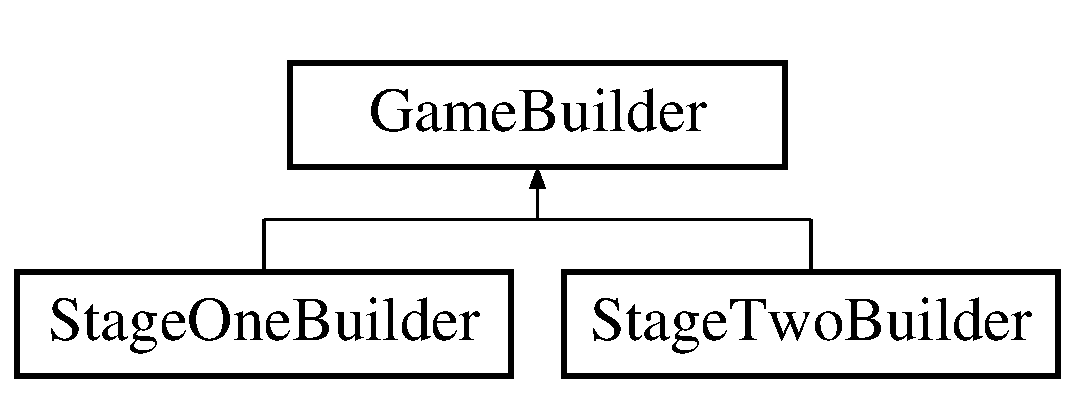
\includegraphics[height=2.000000cm]{class_game_builder}
\end{center}
\end{figure}
\subsection*{Public Member Functions}
\begin{DoxyCompactItemize}
\item 
virtual \mbox{\hyperlink{class_game_builder_ad817a2588d910c2798dfb27808c29d48}{$\sim$\+Game\+Builder}} ()
\item 
\mbox{\hyperlink{class_game_builder_a1540d75dc9f7beb42a95bbc083f86ae1}{Game\+Builder}} (\mbox{\hyperlink{class_abstract_stage_factory}{Abstract\+Stage\+Factory}} $\ast$factory)
\item 
virtual void \mbox{\hyperlink{class_game_builder_a836186637bd2f7844f7dfac0135d833b}{add\+Ball}} (Q\+Json\+Object \&ball\+Data)=0
\begin{DoxyCompactList}\small\item\em add\+Ball creates a ball to the current game being buil \end{DoxyCompactList}\item 
virtual void \mbox{\hyperlink{class_game_builder_a65fb629009c18956a8d592352eda1eb5}{add\+Table}} (Q\+Json\+Object \&table\+Data)=0
\begin{DoxyCompactList}\small\item\em add\+Table creates a table to the current game being built \end{DoxyCompactList}\item 
virtual \mbox{\hyperlink{class_game}{Game}} $\ast$ \mbox{\hyperlink{class_game_builder_a490e3dbb7f8289edb2a080a3383f8607}{get\+Result}} ()
\begin{DoxyCompactList}\small\item\em get\+Result -\/ retrieve the built object \end{DoxyCompactList}\end{DoxyCompactItemize}
\subsection*{Protected Attributes}
\begin{DoxyCompactItemize}
\item 
\mbox{\hyperlink{class_abstract_stage_factory}{Abstract\+Stage\+Factory}} $\ast$ \mbox{\hyperlink{class_game_builder_a2b8da37dc88d521fc01841a2c308508f}{m\+\_\+factory}} = nullptr
\item 
std\+::vector$<$ \mbox{\hyperlink{class_ball}{Ball}} $\ast$ $>$ $\ast$ \mbox{\hyperlink{class_game_builder_a00bf40f2a9c4c72ff8e9bc94201bb681}{m\+\_\+building\+Balls}} = nullptr
\item 
\mbox{\hyperlink{class_table}{Table}} $\ast$ \mbox{\hyperlink{class_game_builder_a0fe16583df85f0360cfe9b06a7ea3aee}{m\+\_\+building\+Table}} = nullptr
\end{DoxyCompactItemize}


\subsection{Detailed Description}


Definition at line 6 of file gamebuilder.\+h.



\subsection{Constructor \& Destructor Documentation}
\mbox{\Hypertarget{class_game_builder_ad817a2588d910c2798dfb27808c29d48}\label{class_game_builder_ad817a2588d910c2798dfb27808c29d48}} 
\index{Game\+Builder@{Game\+Builder}!````~Game\+Builder@{$\sim$\+Game\+Builder}}
\index{````~Game\+Builder@{$\sim$\+Game\+Builder}!Game\+Builder@{Game\+Builder}}
\subsubsection{\texorpdfstring{$\sim$\+Game\+Builder()}{~GameBuilder()}}
{\footnotesize\ttfamily Game\+Builder\+::$\sim$\+Game\+Builder (\begin{DoxyParamCaption}{ }\end{DoxyParamCaption})\hspace{0.3cm}{\ttfamily [virtual]}}



Definition at line 9 of file gamebuilder.\+cpp.

\mbox{\Hypertarget{class_game_builder_a1540d75dc9f7beb42a95bbc083f86ae1}\label{class_game_builder_a1540d75dc9f7beb42a95bbc083f86ae1}} 
\index{Game\+Builder@{Game\+Builder}!Game\+Builder@{Game\+Builder}}
\index{Game\+Builder@{Game\+Builder}!Game\+Builder@{Game\+Builder}}
\subsubsection{\texorpdfstring{Game\+Builder()}{GameBuilder()}}
{\footnotesize\ttfamily Game\+Builder\+::\+Game\+Builder (\begin{DoxyParamCaption}\item[{\mbox{\hyperlink{class_abstract_stage_factory}{Abstract\+Stage\+Factory}} $\ast$}]{factory }\end{DoxyParamCaption})\hspace{0.3cm}{\ttfamily [inline]}}



Definition at line 13 of file gamebuilder.\+h.



\subsection{Member Function Documentation}
\mbox{\Hypertarget{class_game_builder_a836186637bd2f7844f7dfac0135d833b}\label{class_game_builder_a836186637bd2f7844f7dfac0135d833b}} 
\index{Game\+Builder@{Game\+Builder}!add\+Ball@{add\+Ball}}
\index{add\+Ball@{add\+Ball}!Game\+Builder@{Game\+Builder}}
\subsubsection{\texorpdfstring{add\+Ball()}{addBall()}}
{\footnotesize\ttfamily virtual void Game\+Builder\+::add\+Ball (\begin{DoxyParamCaption}\item[{Q\+Json\+Object \&}]{ball\+Data }\end{DoxyParamCaption})\hspace{0.3cm}{\ttfamily [pure virtual]}}



add\+Ball creates a ball to the current game being buil 


\begin{DoxyParams}{Parameters}
{\em ball\+Data} & -\/ json object that is simply an element of the array of balls provided in the config \\
\hline
\end{DoxyParams}


Implemented in \mbox{\hyperlink{class_stage_one_builder_a9d7931aab89afcfa0b2c23da6fb10bfb}{Stage\+One\+Builder}}, and \mbox{\hyperlink{class_stage_two_builder_a8b2b783294c26b5f40d16bdd54d86301}{Stage\+Two\+Builder}}.

\mbox{\Hypertarget{class_game_builder_a65fb629009c18956a8d592352eda1eb5}\label{class_game_builder_a65fb629009c18956a8d592352eda1eb5}} 
\index{Game\+Builder@{Game\+Builder}!add\+Table@{add\+Table}}
\index{add\+Table@{add\+Table}!Game\+Builder@{Game\+Builder}}
\subsubsection{\texorpdfstring{add\+Table()}{addTable()}}
{\footnotesize\ttfamily virtual void Game\+Builder\+::add\+Table (\begin{DoxyParamCaption}\item[{Q\+Json\+Object \&}]{table\+Data }\end{DoxyParamCaption})\hspace{0.3cm}{\ttfamily [pure virtual]}}



add\+Table creates a table to the current game being built 


\begin{DoxyParams}{Parameters}
{\em table\+Data} & -\/ json object that contains all properties of the table \\
\hline
\end{DoxyParams}


Implemented in \mbox{\hyperlink{class_stage_one_builder_ac8f35ec11ebe31010410bc50b0149ce9}{Stage\+One\+Builder}}, and \mbox{\hyperlink{class_stage_two_builder_a7326ee514e752cab6d994352f5ef68e0}{Stage\+Two\+Builder}}.

\mbox{\Hypertarget{class_game_builder_a490e3dbb7f8289edb2a080a3383f8607}\label{class_game_builder_a490e3dbb7f8289edb2a080a3383f8607}} 
\index{Game\+Builder@{Game\+Builder}!get\+Result@{get\+Result}}
\index{get\+Result@{get\+Result}!Game\+Builder@{Game\+Builder}}
\subsubsection{\texorpdfstring{get\+Result()}{getResult()}}
{\footnotesize\ttfamily \mbox{\hyperlink{class_game}{Game}} $\ast$ Game\+Builder\+::get\+Result (\begin{DoxyParamCaption}{ }\end{DoxyParamCaption})\hspace{0.3cm}{\ttfamily [virtual]}}



get\+Result -\/ retrieve the built object 

\begin{DoxyReturn}{Returns}

\end{DoxyReturn}


Reimplemented in \mbox{\hyperlink{class_stage_two_builder_ac40c00c49b18b7c4f83f4474a8cd9c73}{Stage\+Two\+Builder}}.



Definition at line 19 of file gamebuilder.\+cpp.



\subsection{Member Data Documentation}
\mbox{\Hypertarget{class_game_builder_a00bf40f2a9c4c72ff8e9bc94201bb681}\label{class_game_builder_a00bf40f2a9c4c72ff8e9bc94201bb681}} 
\index{Game\+Builder@{Game\+Builder}!m\+\_\+building\+Balls@{m\+\_\+building\+Balls}}
\index{m\+\_\+building\+Balls@{m\+\_\+building\+Balls}!Game\+Builder@{Game\+Builder}}
\subsubsection{\texorpdfstring{m\+\_\+building\+Balls}{m\_buildingBalls}}
{\footnotesize\ttfamily std\+::vector$<$\mbox{\hyperlink{class_ball}{Ball}}$\ast$$>$$\ast$ Game\+Builder\+::m\+\_\+building\+Balls = nullptr\hspace{0.3cm}{\ttfamily [protected]}}



Definition at line 9 of file gamebuilder.\+h.

\mbox{\Hypertarget{class_game_builder_a0fe16583df85f0360cfe9b06a7ea3aee}\label{class_game_builder_a0fe16583df85f0360cfe9b06a7ea3aee}} 
\index{Game\+Builder@{Game\+Builder}!m\+\_\+building\+Table@{m\+\_\+building\+Table}}
\index{m\+\_\+building\+Table@{m\+\_\+building\+Table}!Game\+Builder@{Game\+Builder}}
\subsubsection{\texorpdfstring{m\+\_\+building\+Table}{m\_buildingTable}}
{\footnotesize\ttfamily \mbox{\hyperlink{class_table}{Table}}$\ast$ Game\+Builder\+::m\+\_\+building\+Table = nullptr\hspace{0.3cm}{\ttfamily [protected]}}



Definition at line 10 of file gamebuilder.\+h.

\mbox{\Hypertarget{class_game_builder_a2b8da37dc88d521fc01841a2c308508f}\label{class_game_builder_a2b8da37dc88d521fc01841a2c308508f}} 
\index{Game\+Builder@{Game\+Builder}!m\+\_\+factory@{m\+\_\+factory}}
\index{m\+\_\+factory@{m\+\_\+factory}!Game\+Builder@{Game\+Builder}}
\subsubsection{\texorpdfstring{m\+\_\+factory}{m\_factory}}
{\footnotesize\ttfamily \mbox{\hyperlink{class_abstract_stage_factory}{Abstract\+Stage\+Factory}}$\ast$ Game\+Builder\+::m\+\_\+factory = nullptr\hspace{0.3cm}{\ttfamily [protected]}}



Definition at line 8 of file gamebuilder.\+h.



The documentation for this class was generated from the following files\+:\begin{DoxyCompactItemize}
\item 
\mbox{\hyperlink{gamebuilder_8h}{gamebuilder.\+h}}\item 
\mbox{\hyperlink{gamebuilder_8cpp}{gamebuilder.\+cpp}}\end{DoxyCompactItemize}

\hypertarget{class_game_director}{}\section{Game\+Director Class Reference}
\label{class_game_director}\index{Game\+Director@{Game\+Director}}
\subsection*{Public Member Functions}
\begin{DoxyCompactItemize}
\item 
\mbox{\Hypertarget{class_game_director_a3ac974d917a3cff7a7873bcf9bbfc2ce}\label{class_game_director_a3ac974d917a3cff7a7873bcf9bbfc2ce}} 
{\bfseries Game\+Director} (Q\+Json\+Object $\ast$conf)
\item 
void \mbox{\hyperlink{class_game_director_af849b0b8309680e7eb53cc1803895aab}{set\+Builder}} (\mbox{\hyperlink{class_game_builder}{Game\+Builder}} $\ast$new\+Builder)
\begin{DoxyCompactList}\small\item\em set\+Builder -\/ change which builder should be used for construction \end{DoxyCompactList}\item 
\mbox{\hyperlink{class_game}{Game}} $\ast$ \mbox{\hyperlink{class_game_director_a39ad3747cf1b3bf8a6e335167f73d04b}{create\+Game}} ()
\begin{DoxyCompactList}\small\item\em create\+Game -\/ retrieve the building that our owned builder created \end{DoxyCompactList}\end{DoxyCompactItemize}


\subsection{Member Function Documentation}
\mbox{\Hypertarget{class_game_director_a39ad3747cf1b3bf8a6e335167f73d04b}\label{class_game_director_a39ad3747cf1b3bf8a6e335167f73d04b}} 
\index{Game\+Director@{Game\+Director}!create\+Game@{create\+Game}}
\index{create\+Game@{create\+Game}!Game\+Director@{Game\+Director}}
\subsubsection{\texorpdfstring{create\+Game()}{createGame()}}
{\footnotesize\ttfamily \mbox{\hyperlink{class_game}{Game}} $\ast$ Game\+Director\+::create\+Game (\begin{DoxyParamCaption}{ }\end{DoxyParamCaption})}



create\+Game -\/ retrieve the building that our owned builder created 

\begin{DoxyReturn}{Returns}
-\/ the newly created game 
\end{DoxyReturn}
\mbox{\Hypertarget{class_game_director_af849b0b8309680e7eb53cc1803895aab}\label{class_game_director_af849b0b8309680e7eb53cc1803895aab}} 
\index{Game\+Director@{Game\+Director}!set\+Builder@{set\+Builder}}
\index{set\+Builder@{set\+Builder}!Game\+Director@{Game\+Director}}
\subsubsection{\texorpdfstring{set\+Builder()}{setBuilder()}}
{\footnotesize\ttfamily void Game\+Director\+::set\+Builder (\begin{DoxyParamCaption}\item[{\mbox{\hyperlink{class_game_builder}{Game\+Builder}} $\ast$}]{new\+Builder }\end{DoxyParamCaption})\hspace{0.3cm}{\ttfamily [inline]}}



set\+Builder -\/ change which builder should be used for construction 


\begin{DoxyParams}{Parameters}
{\em new\+Builder} & -\/ the new builder \\
\hline
\end{DoxyParams}


The documentation for this class was generated from the following files\+:\begin{DoxyCompactItemize}
\item 
gamebuilder.\+h\item 
gamebuilder.\+cpp\end{DoxyCompactItemize}

\hypertarget{class_pocket}{}\section{Pocket Class Reference}
\label{class_pocket}\index{Pocket@{Pocket}}


{\ttfamily \#include $<$pocket.\+h$>$}

\subsection*{Public Member Functions}
\begin{DoxyCompactItemize}
\item 
\mbox{\hyperlink{class_pocket_a967b7b80a4a7aba6b56509d1d0e28a24}{Pocket}} (double radius, Q\+Vector2D pos)
\item 
void \mbox{\hyperlink{class_pocket_ab6114f9e08389b3ccdba3676275479e7}{render}} (Q\+Painter \&painter, const Q\+Vector2D \&offset)
\begin{DoxyCompactList}\small\item\em render -\/ draw the pocket to the screen with the provided brush and offset \end{DoxyCompactList}\item 
bool \mbox{\hyperlink{class_pocket_ac01b76c9853e24904296d467ceeaa821}{contains}} (const Q\+Vector2D \&center, const double \&radius)
\item 
void \mbox{\hyperlink{class_pocket_a4ba8a5305df04f95a25a6c7027b05c2b}{increment\+Sunk}} ()
\end{DoxyCompactItemize}


\subsection{Detailed Description}


Definition at line 8 of file pocket.\+h.



\subsection{Constructor \& Destructor Documentation}
\mbox{\Hypertarget{class_pocket_a967b7b80a4a7aba6b56509d1d0e28a24}\label{class_pocket_a967b7b80a4a7aba6b56509d1d0e28a24}} 
\index{Pocket@{Pocket}!Pocket@{Pocket}}
\index{Pocket@{Pocket}!Pocket@{Pocket}}
\subsubsection{\texorpdfstring{Pocket()}{Pocket()}}
{\footnotesize\ttfamily Pocket\+::\+Pocket (\begin{DoxyParamCaption}\item[{double}]{radius,  }\item[{Q\+Vector2D}]{pos }\end{DoxyParamCaption})\hspace{0.3cm}{\ttfamily [inline]}}



Definition at line 17 of file pocket.\+h.



\subsection{Member Function Documentation}
\mbox{\Hypertarget{class_pocket_ac01b76c9853e24904296d467ceeaa821}\label{class_pocket_ac01b76c9853e24904296d467ceeaa821}} 
\index{Pocket@{Pocket}!contains@{contains}}
\index{contains@{contains}!Pocket@{Pocket}}
\subsubsection{\texorpdfstring{contains()}{contains()}}
{\footnotesize\ttfamily bool Pocket\+::contains (\begin{DoxyParamCaption}\item[{const Q\+Vector2D \&}]{center,  }\item[{const double \&}]{radius }\end{DoxyParamCaption})\hspace{0.3cm}{\ttfamily [inline]}}



Definition at line 27 of file pocket.\+h.

\mbox{\Hypertarget{class_pocket_a4ba8a5305df04f95a25a6c7027b05c2b}\label{class_pocket_a4ba8a5305df04f95a25a6c7027b05c2b}} 
\index{Pocket@{Pocket}!increment\+Sunk@{increment\+Sunk}}
\index{increment\+Sunk@{increment\+Sunk}!Pocket@{Pocket}}
\subsubsection{\texorpdfstring{increment\+Sunk()}{incrementSunk()}}
{\footnotesize\ttfamily void Pocket\+::increment\+Sunk (\begin{DoxyParamCaption}{ }\end{DoxyParamCaption})\hspace{0.3cm}{\ttfamily [inline]}}



Definition at line 32 of file pocket.\+h.

\mbox{\Hypertarget{class_pocket_ab6114f9e08389b3ccdba3676275479e7}\label{class_pocket_ab6114f9e08389b3ccdba3676275479e7}} 
\index{Pocket@{Pocket}!render@{render}}
\index{render@{render}!Pocket@{Pocket}}
\subsubsection{\texorpdfstring{render()}{render()}}
{\footnotesize\ttfamily void Pocket\+::render (\begin{DoxyParamCaption}\item[{Q\+Painter \&}]{painter,  }\item[{const Q\+Vector2D \&}]{offset }\end{DoxyParamCaption})}



render -\/ draw the pocket to the screen with the provided brush and offset 


\begin{DoxyParams}{Parameters}
{\em painter} & -\/ the brush to paint with \\
\hline
{\em offset} & -\/ the offset from the window \\
\hline
\end{DoxyParams}


Definition at line 4 of file pocket.\+cpp.



The documentation for this class was generated from the following files\+:\begin{DoxyCompactItemize}
\item 
\mbox{\hyperlink{pocket_8h}{pocket.\+h}}\item 
\mbox{\hyperlink{pocket_8cpp}{pocket.\+cpp}}\end{DoxyCompactItemize}

\hypertarget{struct_ball_sparkle_decorator_1_1_sparkle}{}\section{Ball\+Sparkle\+Decorator\+:\+:Sparkle Struct Reference}
\label{struct_ball_sparkle_decorator_1_1_sparkle}\index{Ball\+Sparkle\+Decorator\+::\+Sparkle@{Ball\+Sparkle\+Decorator\+::\+Sparkle}}


{\ttfamily \#include $<$balldecorator.\+h$>$}

\subsection*{Public Member Functions}
\begin{DoxyCompactItemize}
\item 
\mbox{\hyperlink{struct_ball_sparkle_decorator_1_1_sparkle_a3c722e501faf223889464bd622375c11}{Sparkle}} (Q\+PointF \mbox{\hyperlink{struct_ball_sparkle_decorator_1_1_sparkle_aeb4b735006a31fa11fa78394a4848236}{pos}}, double \mbox{\hyperlink{struct_ball_sparkle_decorator_1_1_sparkle_a44963032a6ce95c5b552d4c5159f88c2}{opacity}}=1.\+0)
\end{DoxyCompactItemize}
\subsection*{Public Attributes}
\begin{DoxyCompactItemize}
\item 
Q\+PointF \mbox{\hyperlink{struct_ball_sparkle_decorator_1_1_sparkle_aeb4b735006a31fa11fa78394a4848236}{pos}}
\item 
double \mbox{\hyperlink{struct_ball_sparkle_decorator_1_1_sparkle_a44963032a6ce95c5b552d4c5159f88c2}{opacity}} = 1.\+0
\end{DoxyCompactItemize}
\subsection*{Static Public Attributes}
\begin{DoxyCompactItemize}
\item 
static constexpr double \mbox{\hyperlink{struct_ball_sparkle_decorator_1_1_sparkle_a6602f6013f4b6d436cf07a67c9a2b98d}{width}} = 5.\+0
\item 
static constexpr double \mbox{\hyperlink{struct_ball_sparkle_decorator_1_1_sparkle_a3098571dbcb489f4821ac0446ef18d26}{height}} = 5.\+0
\end{DoxyCompactItemize}


\subsection{Detailed Description}


Definition at line 85 of file balldecorator.\+h.



\subsection{Constructor \& Destructor Documentation}
\mbox{\Hypertarget{struct_ball_sparkle_decorator_1_1_sparkle_a3c722e501faf223889464bd622375c11}\label{struct_ball_sparkle_decorator_1_1_sparkle_a3c722e501faf223889464bd622375c11}} 
\index{Ball\+Sparkle\+Decorator\+::\+Sparkle@{Ball\+Sparkle\+Decorator\+::\+Sparkle}!Sparkle@{Sparkle}}
\index{Sparkle@{Sparkle}!Ball\+Sparkle\+Decorator\+::\+Sparkle@{Ball\+Sparkle\+Decorator\+::\+Sparkle}}
\subsubsection{\texorpdfstring{Sparkle()}{Sparkle()}}
{\footnotesize\ttfamily Ball\+Sparkle\+Decorator\+::\+Sparkle\+::\+Sparkle (\begin{DoxyParamCaption}\item[{Q\+PointF}]{pos,  }\item[{double}]{opacity = {\ttfamily 1.0} }\end{DoxyParamCaption})\hspace{0.3cm}{\ttfamily [inline]}}



Definition at line 86 of file balldecorator.\+h.



\subsection{Member Data Documentation}
\mbox{\Hypertarget{struct_ball_sparkle_decorator_1_1_sparkle_a3098571dbcb489f4821ac0446ef18d26}\label{struct_ball_sparkle_decorator_1_1_sparkle_a3098571dbcb489f4821ac0446ef18d26}} 
\index{Ball\+Sparkle\+Decorator\+::\+Sparkle@{Ball\+Sparkle\+Decorator\+::\+Sparkle}!height@{height}}
\index{height@{height}!Ball\+Sparkle\+Decorator\+::\+Sparkle@{Ball\+Sparkle\+Decorator\+::\+Sparkle}}
\subsubsection{\texorpdfstring{height}{height}}
{\footnotesize\ttfamily constexpr double Ball\+Sparkle\+Decorator\+::\+Sparkle\+::height = 5.\+0\hspace{0.3cm}{\ttfamily [static]}}



Definition at line 92 of file balldecorator.\+h.

\mbox{\Hypertarget{struct_ball_sparkle_decorator_1_1_sparkle_a44963032a6ce95c5b552d4c5159f88c2}\label{struct_ball_sparkle_decorator_1_1_sparkle_a44963032a6ce95c5b552d4c5159f88c2}} 
\index{Ball\+Sparkle\+Decorator\+::\+Sparkle@{Ball\+Sparkle\+Decorator\+::\+Sparkle}!opacity@{opacity}}
\index{opacity@{opacity}!Ball\+Sparkle\+Decorator\+::\+Sparkle@{Ball\+Sparkle\+Decorator\+::\+Sparkle}}
\subsubsection{\texorpdfstring{opacity}{opacity}}
{\footnotesize\ttfamily double Ball\+Sparkle\+Decorator\+::\+Sparkle\+::opacity = 1.\+0}



Definition at line 90 of file balldecorator.\+h.

\mbox{\Hypertarget{struct_ball_sparkle_decorator_1_1_sparkle_aeb4b735006a31fa11fa78394a4848236}\label{struct_ball_sparkle_decorator_1_1_sparkle_aeb4b735006a31fa11fa78394a4848236}} 
\index{Ball\+Sparkle\+Decorator\+::\+Sparkle@{Ball\+Sparkle\+Decorator\+::\+Sparkle}!pos@{pos}}
\index{pos@{pos}!Ball\+Sparkle\+Decorator\+::\+Sparkle@{Ball\+Sparkle\+Decorator\+::\+Sparkle}}
\subsubsection{\texorpdfstring{pos}{pos}}
{\footnotesize\ttfamily Q\+PointF Ball\+Sparkle\+Decorator\+::\+Sparkle\+::pos}



Definition at line 89 of file balldecorator.\+h.

\mbox{\Hypertarget{struct_ball_sparkle_decorator_1_1_sparkle_a6602f6013f4b6d436cf07a67c9a2b98d}\label{struct_ball_sparkle_decorator_1_1_sparkle_a6602f6013f4b6d436cf07a67c9a2b98d}} 
\index{Ball\+Sparkle\+Decorator\+::\+Sparkle@{Ball\+Sparkle\+Decorator\+::\+Sparkle}!width@{width}}
\index{width@{width}!Ball\+Sparkle\+Decorator\+::\+Sparkle@{Ball\+Sparkle\+Decorator\+::\+Sparkle}}
\subsubsection{\texorpdfstring{width}{width}}
{\footnotesize\ttfamily constexpr double Ball\+Sparkle\+Decorator\+::\+Sparkle\+::width = 5.\+0\hspace{0.3cm}{\ttfamily [static]}}



Definition at line 91 of file balldecorator.\+h.



The documentation for this struct was generated from the following file\+:\begin{DoxyCompactItemize}
\item 
\mbox{\hyperlink{balldecorator_8h}{balldecorator.\+h}}\end{DoxyCompactItemize}

\hypertarget{class_stage_one_ball}{}\section{Stage\+One\+Ball Class Reference}
\label{class_stage_one_ball}\index{Stage\+One\+Ball@{Stage\+One\+Ball}}


{\ttfamily \#include $<$ball.\+h$>$}

Inheritance diagram for Stage\+One\+Ball\+:\begin{figure}[H]
\begin{center}
\leavevmode
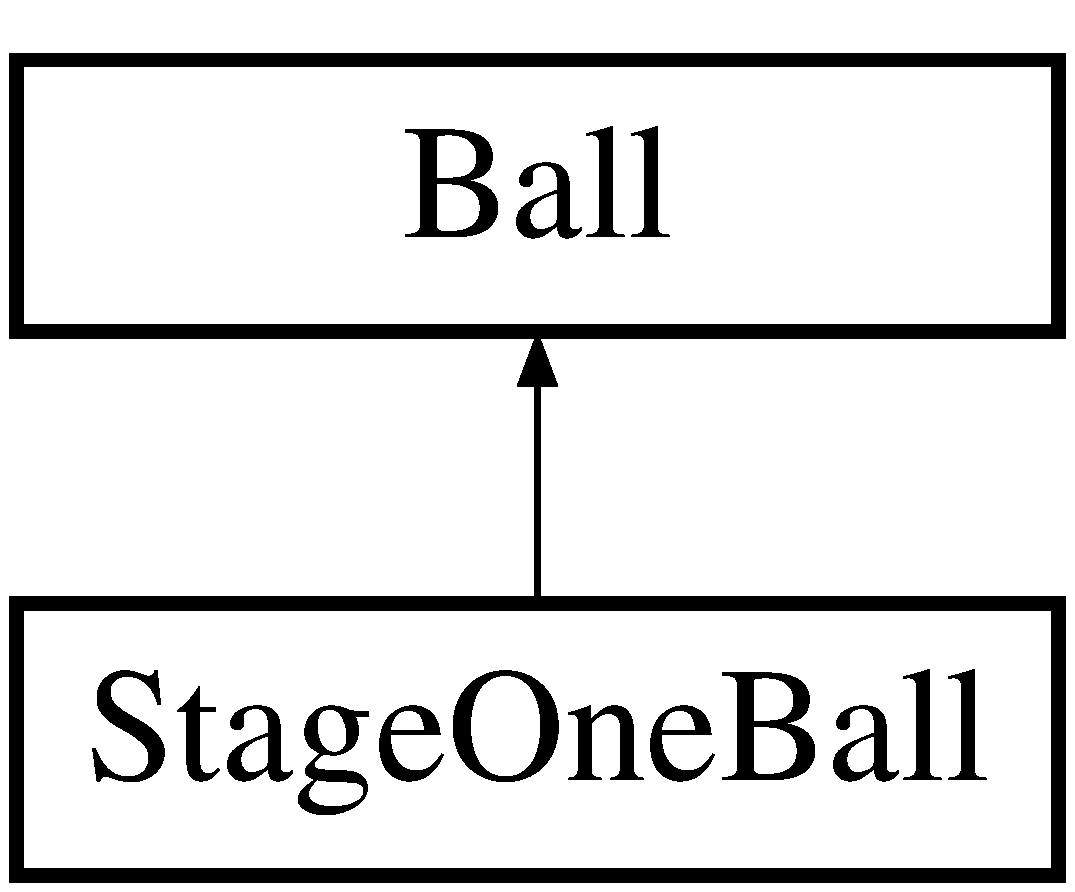
\includegraphics[height=2.000000cm]{class_stage_one_ball}
\end{center}
\end{figure}
\subsection*{Public Member Functions}
\begin{DoxyCompactItemize}
\item 
\mbox{\hyperlink{class_stage_one_ball_a70fd661f3b92f3e4745d4963b9b3ec80}{Stage\+One\+Ball}} (Q\+Color colour, Q\+Vector2D position, Q\+Vector2D velocity, double mass, int radius)
\item 
void \mbox{\hyperlink{class_stage_one_ball_aa4f7f52cb8946b59c201d724dc0dc5bd}{render}} (Q\+Painter \&painter, const Q\+Vector2D \&offset) override
\begin{DoxyCompactList}\small\item\em render -\/ draw the ball to the screen \end{DoxyCompactList}\end{DoxyCompactItemize}
\subsection*{Additional Inherited Members}


\subsection{Detailed Description}


Definition at line 60 of file ball.\+h.



\subsection{Constructor \& Destructor Documentation}
\mbox{\Hypertarget{class_stage_one_ball_a70fd661f3b92f3e4745d4963b9b3ec80}\label{class_stage_one_ball_a70fd661f3b92f3e4745d4963b9b3ec80}} 
\index{Stage\+One\+Ball@{Stage\+One\+Ball}!Stage\+One\+Ball@{Stage\+One\+Ball}}
\index{Stage\+One\+Ball@{Stage\+One\+Ball}!Stage\+One\+Ball@{Stage\+One\+Ball}}
\subsubsection{\texorpdfstring{Stage\+One\+Ball()}{StageOneBall()}}
{\footnotesize\ttfamily Stage\+One\+Ball\+::\+Stage\+One\+Ball (\begin{DoxyParamCaption}\item[{Q\+Color}]{colour,  }\item[{Q\+Vector2D}]{position,  }\item[{Q\+Vector2D}]{velocity,  }\item[{double}]{mass,  }\item[{int}]{radius }\end{DoxyParamCaption})\hspace{0.3cm}{\ttfamily [inline]}}



Definition at line 62 of file ball.\+h.



\subsection{Member Function Documentation}
\mbox{\Hypertarget{class_stage_one_ball_aa4f7f52cb8946b59c201d724dc0dc5bd}\label{class_stage_one_ball_aa4f7f52cb8946b59c201d724dc0dc5bd}} 
\index{Stage\+One\+Ball@{Stage\+One\+Ball}!render@{render}}
\index{render@{render}!Stage\+One\+Ball@{Stage\+One\+Ball}}
\subsubsection{\texorpdfstring{render()}{render()}}
{\footnotesize\ttfamily void Stage\+One\+Ball\+::render (\begin{DoxyParamCaption}\item[{Q\+Painter \&}]{painter,  }\item[{const Q\+Vector2D \&}]{offset }\end{DoxyParamCaption})\hspace{0.3cm}{\ttfamily [override]}, {\ttfamily [virtual]}}



render -\/ draw the ball to the screen 


\begin{DoxyParams}{Parameters}
{\em painter} & -\/ Q\+Painter that is owned by the dialog \\
\hline
\end{DoxyParams}


Implements \mbox{\hyperlink{class_ball_a307773aaa59aee90cef8767b0c22deca}{Ball}}.



Definition at line 4 of file ball.\+cpp.



The documentation for this class was generated from the following files\+:\begin{DoxyCompactItemize}
\item 
\mbox{\hyperlink{ball_8h}{ball.\+h}}\item 
\mbox{\hyperlink{ball_8cpp}{ball.\+cpp}}\end{DoxyCompactItemize}

\hypertarget{class_stage_one_builder}{}\section{Stage\+One\+Builder Class Reference}
\label{class_stage_one_builder}\index{Stage\+One\+Builder@{Stage\+One\+Builder}}


{\ttfamily \#include $<$gamebuilder.\+h$>$}

Inheritance diagram for Stage\+One\+Builder\+:\begin{figure}[H]
\begin{center}
\leavevmode
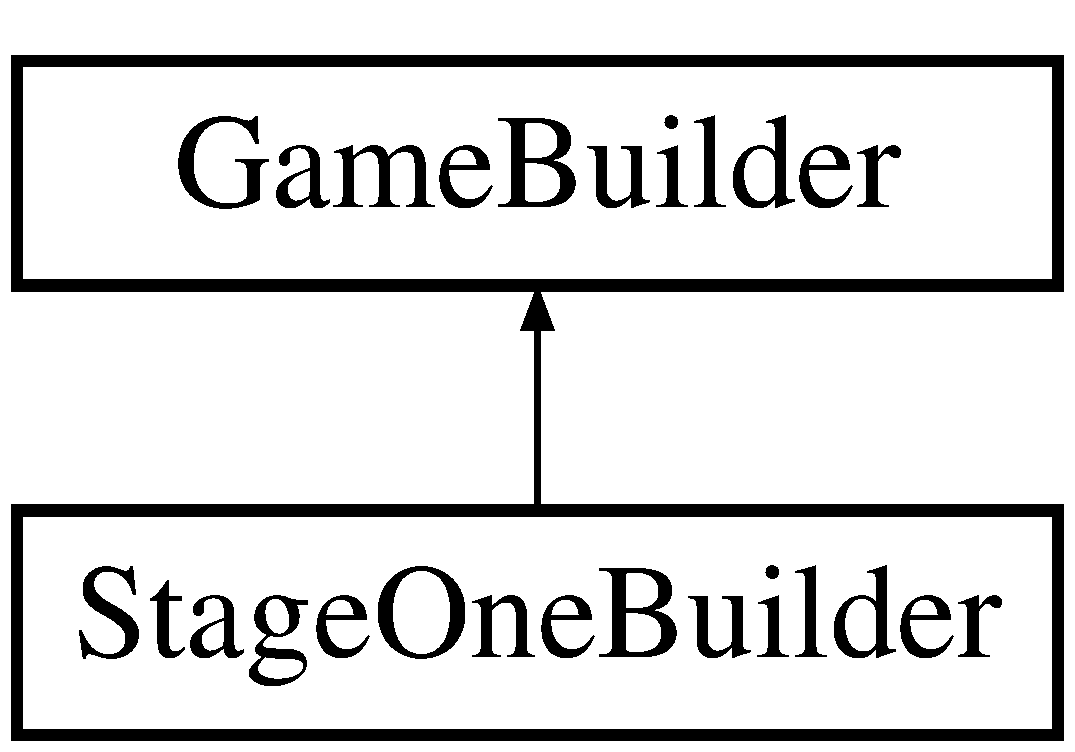
\includegraphics[height=2.000000cm]{class_stage_one_builder}
\end{center}
\end{figure}
\subsection*{Public Member Functions}
\begin{DoxyCompactItemize}
\item 
\mbox{\hyperlink{class_stage_one_builder_a1008b1e1d473b4c3e3db2fca1122d4b0}{$\sim$\+Stage\+One\+Builder}} ()
\item 
\mbox{\hyperlink{class_stage_one_builder_aaeaf7f5af709b6530e95db25bab3af13}{Stage\+One\+Builder}} ()
\item 
void \mbox{\hyperlink{class_stage_one_builder_a9d7931aab89afcfa0b2c23da6fb10bfb}{add\+Ball}} (Q\+Json\+Object \&ball\+Data) override
\begin{DoxyCompactList}\small\item\em add\+Ball creates a ball to the current game being built \end{DoxyCompactList}\item 
void \mbox{\hyperlink{class_stage_one_builder_ac8f35ec11ebe31010410bc50b0149ce9}{add\+Table}} (Q\+Json\+Object \&table\+Data) override
\begin{DoxyCompactList}\small\item\em add\+Table creates a table to the current game being built \end{DoxyCompactList}\end{DoxyCompactItemize}
\subsection*{Additional Inherited Members}


\subsection{Detailed Description}


Definition at line 33 of file gamebuilder.\+h.



\subsection{Constructor \& Destructor Documentation}
\mbox{\Hypertarget{class_stage_one_builder_a1008b1e1d473b4c3e3db2fca1122d4b0}\label{class_stage_one_builder_a1008b1e1d473b4c3e3db2fca1122d4b0}} 
\index{Stage\+One\+Builder@{Stage\+One\+Builder}!````~Stage\+One\+Builder@{$\sim$\+Stage\+One\+Builder}}
\index{````~Stage\+One\+Builder@{$\sim$\+Stage\+One\+Builder}!Stage\+One\+Builder@{Stage\+One\+Builder}}
\subsubsection{\texorpdfstring{$\sim$\+Stage\+One\+Builder()}{~StageOneBuilder()}}
{\footnotesize\ttfamily Stage\+One\+Builder\+::$\sim$\+Stage\+One\+Builder (\begin{DoxyParamCaption}{ }\end{DoxyParamCaption})\hspace{0.3cm}{\ttfamily [inline]}}



Definition at line 35 of file gamebuilder.\+h.

\mbox{\Hypertarget{class_stage_one_builder_aaeaf7f5af709b6530e95db25bab3af13}\label{class_stage_one_builder_aaeaf7f5af709b6530e95db25bab3af13}} 
\index{Stage\+One\+Builder@{Stage\+One\+Builder}!Stage\+One\+Builder@{Stage\+One\+Builder}}
\index{Stage\+One\+Builder@{Stage\+One\+Builder}!Stage\+One\+Builder@{Stage\+One\+Builder}}
\subsubsection{\texorpdfstring{Stage\+One\+Builder()}{StageOneBuilder()}}
{\footnotesize\ttfamily Stage\+One\+Builder\+::\+Stage\+One\+Builder (\begin{DoxyParamCaption}{ }\end{DoxyParamCaption})\hspace{0.3cm}{\ttfamily [inline]}}



Definition at line 36 of file gamebuilder.\+h.



\subsection{Member Function Documentation}
\mbox{\Hypertarget{class_stage_one_builder_a9d7931aab89afcfa0b2c23da6fb10bfb}\label{class_stage_one_builder_a9d7931aab89afcfa0b2c23da6fb10bfb}} 
\index{Stage\+One\+Builder@{Stage\+One\+Builder}!add\+Ball@{add\+Ball}}
\index{add\+Ball@{add\+Ball}!Stage\+One\+Builder@{Stage\+One\+Builder}}
\subsubsection{\texorpdfstring{add\+Ball()}{addBall()}}
{\footnotesize\ttfamily void Stage\+One\+Builder\+::add\+Ball (\begin{DoxyParamCaption}\item[{Q\+Json\+Object \&}]{ball\+Data }\end{DoxyParamCaption})\hspace{0.3cm}{\ttfamily [override]}, {\ttfamily [virtual]}}



add\+Ball creates a ball to the current game being built 


\begin{DoxyParams}{Parameters}
{\em ball\+Data} & -\/ json object that is simply an element of the array of balls provided in the config \\
\hline
\end{DoxyParams}


Implements \mbox{\hyperlink{class_game_builder_a836186637bd2f7844f7dfac0135d833b}{Game\+Builder}}.



Definition at line 39 of file gamebuilder.\+cpp.

\mbox{\Hypertarget{class_stage_one_builder_ac8f35ec11ebe31010410bc50b0149ce9}\label{class_stage_one_builder_ac8f35ec11ebe31010410bc50b0149ce9}} 
\index{Stage\+One\+Builder@{Stage\+One\+Builder}!add\+Table@{add\+Table}}
\index{add\+Table@{add\+Table}!Stage\+One\+Builder@{Stage\+One\+Builder}}
\subsubsection{\texorpdfstring{add\+Table()}{addTable()}}
{\footnotesize\ttfamily void Stage\+One\+Builder\+::add\+Table (\begin{DoxyParamCaption}\item[{Q\+Json\+Object \&}]{table\+Data }\end{DoxyParamCaption})\hspace{0.3cm}{\ttfamily [override]}, {\ttfamily [virtual]}}



add\+Table creates a table to the current game being built 


\begin{DoxyParams}{Parameters}
{\em table\+Data} & -\/ json object that contains all properties of the table \\
\hline
\end{DoxyParams}


Implements \mbox{\hyperlink{class_game_builder_a65fb629009c18956a8d592352eda1eb5}{Game\+Builder}}.



Definition at line 47 of file gamebuilder.\+cpp.



The documentation for this class was generated from the following files\+:\begin{DoxyCompactItemize}
\item 
\mbox{\hyperlink{gamebuilder_8h}{gamebuilder.\+h}}\item 
\mbox{\hyperlink{gamebuilder_8cpp}{gamebuilder.\+cpp}}\end{DoxyCompactItemize}

\hypertarget{class_stage_one_factory}{}\section{Stage\+One\+Factory Class Reference}
\label{class_stage_one_factory}\index{Stage\+One\+Factory@{Stage\+One\+Factory}}


{\ttfamily \#include $<$stageonefactory.\+h$>$}

Inheritance diagram for Stage\+One\+Factory\+:\begin{figure}[H]
\begin{center}
\leavevmode
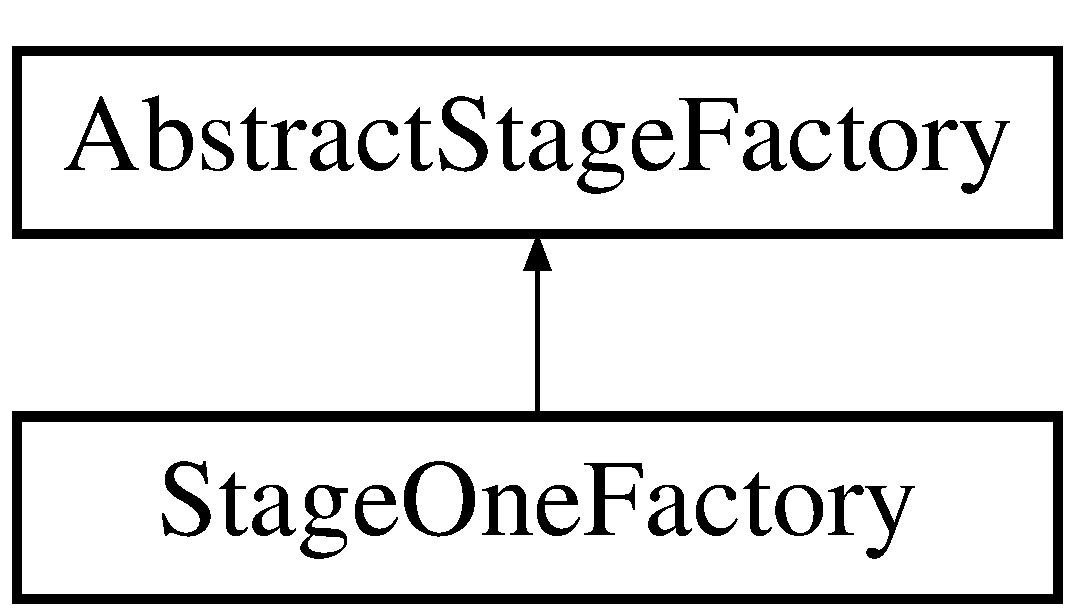
\includegraphics[height=2.000000cm]{class_stage_one_factory}
\end{center}
\end{figure}
\subsection*{Public Member Functions}
\begin{DoxyCompactItemize}
\item 
virtual \mbox{\hyperlink{class_ball}{Ball}} $\ast$ \mbox{\hyperlink{class_stage_one_factory_a8a89031bc805b70d93e942275777394d}{make\+Ball}} (const Q\+Json\+Object \&ball\+Data) override
\begin{DoxyCompactList}\small\item\em make\+Ball -\/ construct a ball based on json \end{DoxyCompactList}\item 
virtual \mbox{\hyperlink{class_table}{Table}} $\ast$ \mbox{\hyperlink{class_stage_one_factory_a31e02c98e5c428f0e1ac0a36e641310d}{make\+Table}} (const Q\+Json\+Object \&table\+Data) override
\begin{DoxyCompactList}\small\item\em make\+Table -\/ construct a table based on json \end{DoxyCompactList}\item 
virtual \mbox{\hyperlink{class_pocket}{Pocket}} $\ast$ \mbox{\hyperlink{class_stage_one_factory_ab9d7b7d74b61a2fd6c96562a67dc2fe8}{make\+Pocket}} (const Q\+Json\+Object \&) override
\begin{DoxyCompactList}\small\item\em make\+Pocket -\/ construct a pocket based on json \end{DoxyCompactList}\end{DoxyCompactItemize}


\subsection{Detailed Description}


Definition at line 4 of file stageonefactory.\+h.



\subsection{Member Function Documentation}
\mbox{\Hypertarget{class_stage_one_factory_a8a89031bc805b70d93e942275777394d}\label{class_stage_one_factory_a8a89031bc805b70d93e942275777394d}} 
\index{Stage\+One\+Factory@{Stage\+One\+Factory}!make\+Ball@{make\+Ball}}
\index{make\+Ball@{make\+Ball}!Stage\+One\+Factory@{Stage\+One\+Factory}}
\subsubsection{\texorpdfstring{make\+Ball()}{makeBall()}}
{\footnotesize\ttfamily \mbox{\hyperlink{class_ball}{Ball}} $\ast$ Stage\+One\+Factory\+::make\+Ball (\begin{DoxyParamCaption}\item[{const Q\+Json\+Object \&}]{ball\+Data }\end{DoxyParamCaption})\hspace{0.3cm}{\ttfamily [override]}, {\ttfamily [virtual]}}



make\+Ball -\/ construct a ball based on json 


\begin{DoxyParams}{Parameters}
{\em ball\+Data} & -\/ our json data for this table \\
\hline
\end{DoxyParams}
\begin{DoxyReturn}{Returns}

\end{DoxyReturn}


Implements \mbox{\hyperlink{class_abstract_stage_factory_a23367d64366e679aaff865620f5ce1ab}{Abstract\+Stage\+Factory}}.



Definition at line 4 of file stageonefactory.\+cpp.

\mbox{\Hypertarget{class_stage_one_factory_ab9d7b7d74b61a2fd6c96562a67dc2fe8}\label{class_stage_one_factory_ab9d7b7d74b61a2fd6c96562a67dc2fe8}} 
\index{Stage\+One\+Factory@{Stage\+One\+Factory}!make\+Pocket@{make\+Pocket}}
\index{make\+Pocket@{make\+Pocket}!Stage\+One\+Factory@{Stage\+One\+Factory}}
\subsubsection{\texorpdfstring{make\+Pocket()}{makePocket()}}
{\footnotesize\ttfamily virtual \mbox{\hyperlink{class_pocket}{Pocket}}$\ast$ Stage\+One\+Factory\+::make\+Pocket (\begin{DoxyParamCaption}\item[{const Q\+Json\+Object \&}]{pocket\+Data }\end{DoxyParamCaption})\hspace{0.3cm}{\ttfamily [inline]}, {\ttfamily [override]}, {\ttfamily [virtual]}}



make\+Pocket -\/ construct a pocket based on json 


\begin{DoxyParams}{Parameters}
{\em pocket\+Data} & -\/ the json \\
\hline
\end{DoxyParams}
\begin{DoxyReturn}{Returns}
newly created pocket 
\end{DoxyReturn}


Implements \mbox{\hyperlink{class_abstract_stage_factory_a6ce57859e00b135049e3b995b7dfc94d}{Abstract\+Stage\+Factory}}.



Definition at line 21 of file stageonefactory.\+h.

\mbox{\Hypertarget{class_stage_one_factory_a31e02c98e5c428f0e1ac0a36e641310d}\label{class_stage_one_factory_a31e02c98e5c428f0e1ac0a36e641310d}} 
\index{Stage\+One\+Factory@{Stage\+One\+Factory}!make\+Table@{make\+Table}}
\index{make\+Table@{make\+Table}!Stage\+One\+Factory@{Stage\+One\+Factory}}
\subsubsection{\texorpdfstring{make\+Table()}{makeTable()}}
{\footnotesize\ttfamily \mbox{\hyperlink{class_table}{Table}} $\ast$ Stage\+One\+Factory\+::make\+Table (\begin{DoxyParamCaption}\item[{const Q\+Json\+Object \&}]{table\+Data }\end{DoxyParamCaption})\hspace{0.3cm}{\ttfamily [override]}, {\ttfamily [virtual]}}



make\+Table -\/ construct a table based on json 


\begin{DoxyParams}{Parameters}
{\em table\+Data} & -\/ our json data for this table \\
\hline
\end{DoxyParams}
\begin{DoxyReturn}{Returns}

\end{DoxyReturn}


Implements \mbox{\hyperlink{class_abstract_stage_factory_a539c855ce9a09e08b7fcb3ffa7f0d3fd}{Abstract\+Stage\+Factory}}.



Definition at line 24 of file stageonefactory.\+cpp.



The documentation for this class was generated from the following files\+:\begin{DoxyCompactItemize}
\item 
\mbox{\hyperlink{stageonefactory_8h}{stageonefactory.\+h}}\item 
\mbox{\hyperlink{stageonefactory_8cpp}{stageonefactory.\+cpp}}\end{DoxyCompactItemize}

\hypertarget{class_stage_one_table}{}\section{Stage\+One\+Table Class Reference}
\label{class_stage_one_table}\index{Stage\+One\+Table@{Stage\+One\+Table}}


{\ttfamily \#include $<$table.\+h$>$}

Inheritance diagram for Stage\+One\+Table\+:\begin{figure}[H]
\begin{center}
\leavevmode
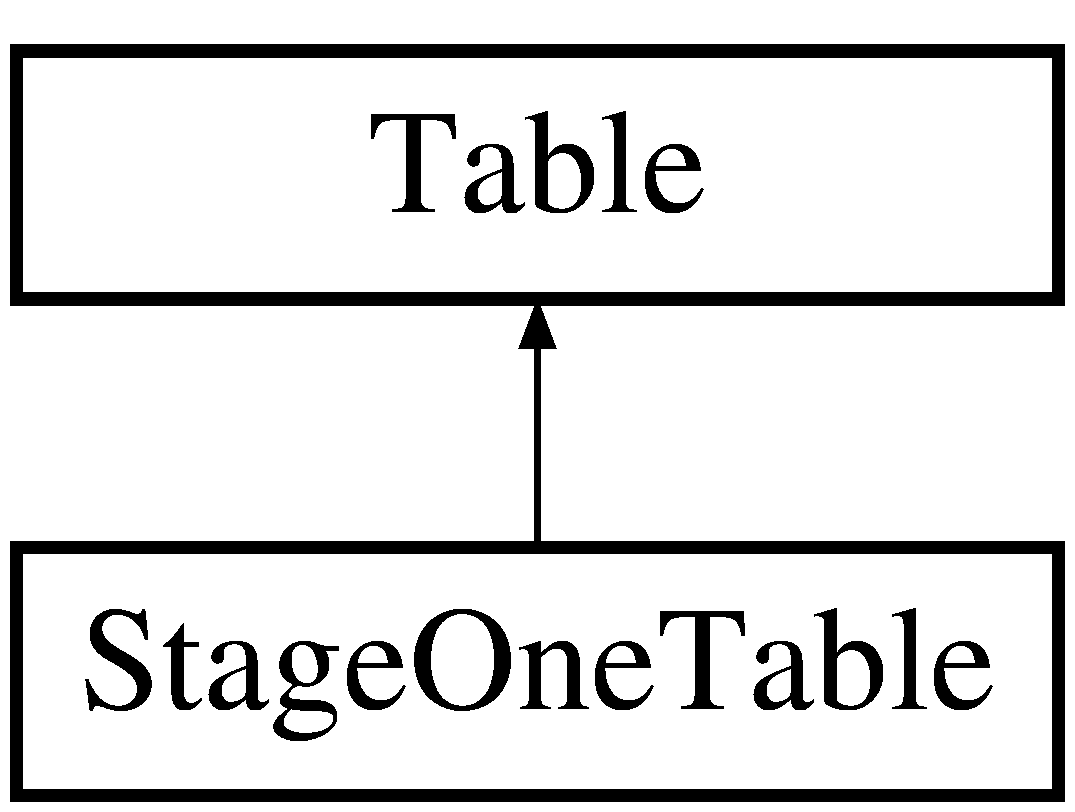
\includegraphics[height=2.000000cm]{class_stage_one_table}
\end{center}
\end{figure}
\subsection*{Public Member Functions}
\begin{DoxyCompactItemize}
\item 
\mbox{\hyperlink{class_stage_one_table_ae7bc7a1e4b873759a40039af326b38b9}{Stage\+One\+Table}} (int width, int height, Q\+Color colour, double friction)
\item 
void \mbox{\hyperlink{class_stage_one_table_a1f6dac59ce45c370f94fb3710f744ceb}{render}} (Q\+Painter \&painter, const Q\+Vector2D \&offset) override
\begin{DoxyCompactList}\small\item\em render -\/ draw the stageonetable to screen using the specified painter \end{DoxyCompactList}\end{DoxyCompactItemize}
\subsection*{Additional Inherited Members}


\subsection{Detailed Description}


Definition at line 34 of file table.\+h.



\subsection{Constructor \& Destructor Documentation}
\mbox{\Hypertarget{class_stage_one_table_ae7bc7a1e4b873759a40039af326b38b9}\label{class_stage_one_table_ae7bc7a1e4b873759a40039af326b38b9}} 
\index{Stage\+One\+Table@{Stage\+One\+Table}!Stage\+One\+Table@{Stage\+One\+Table}}
\index{Stage\+One\+Table@{Stage\+One\+Table}!Stage\+One\+Table@{Stage\+One\+Table}}
\subsubsection{\texorpdfstring{Stage\+One\+Table()}{StageOneTable()}}
{\footnotesize\ttfamily Stage\+One\+Table\+::\+Stage\+One\+Table (\begin{DoxyParamCaption}\item[{int}]{width,  }\item[{int}]{height,  }\item[{Q\+Color}]{colour,  }\item[{double}]{friction }\end{DoxyParamCaption})\hspace{0.3cm}{\ttfamily [inline]}}



Definition at line 37 of file table.\+h.



\subsection{Member Function Documentation}
\mbox{\Hypertarget{class_stage_one_table_a1f6dac59ce45c370f94fb3710f744ceb}\label{class_stage_one_table_a1f6dac59ce45c370f94fb3710f744ceb}} 
\index{Stage\+One\+Table@{Stage\+One\+Table}!render@{render}}
\index{render@{render}!Stage\+One\+Table@{Stage\+One\+Table}}
\subsubsection{\texorpdfstring{render()}{render()}}
{\footnotesize\ttfamily void Stage\+One\+Table\+::render (\begin{DoxyParamCaption}\item[{Q\+Painter \&}]{painter,  }\item[{const Q\+Vector2D \&}]{offset }\end{DoxyParamCaption})\hspace{0.3cm}{\ttfamily [override]}, {\ttfamily [virtual]}}



render -\/ draw the stageonetable to screen using the specified painter 


\begin{DoxyParams}{Parameters}
{\em painter} & -\/ painter to use \\
\hline
\end{DoxyParams}


Implements \mbox{\hyperlink{class_table_a827dac18920a95b3e0ef006183514654}{Table}}.



Definition at line 5 of file table.\+cpp.



The documentation for this class was generated from the following files\+:\begin{DoxyCompactItemize}
\item 
\mbox{\hyperlink{table_8h}{table.\+h}}\item 
\mbox{\hyperlink{table_8cpp}{table.\+cpp}}\end{DoxyCompactItemize}

\hypertarget{class_stage_two_builder}{}\section{Stage\+Two\+Builder Class Reference}
\label{class_stage_two_builder}\index{Stage\+Two\+Builder@{Stage\+Two\+Builder}}


{\ttfamily \#include $<$stagetwobuilder.\+h$>$}

Inheritance diagram for Stage\+Two\+Builder\+:\begin{figure}[H]
\begin{center}
\leavevmode
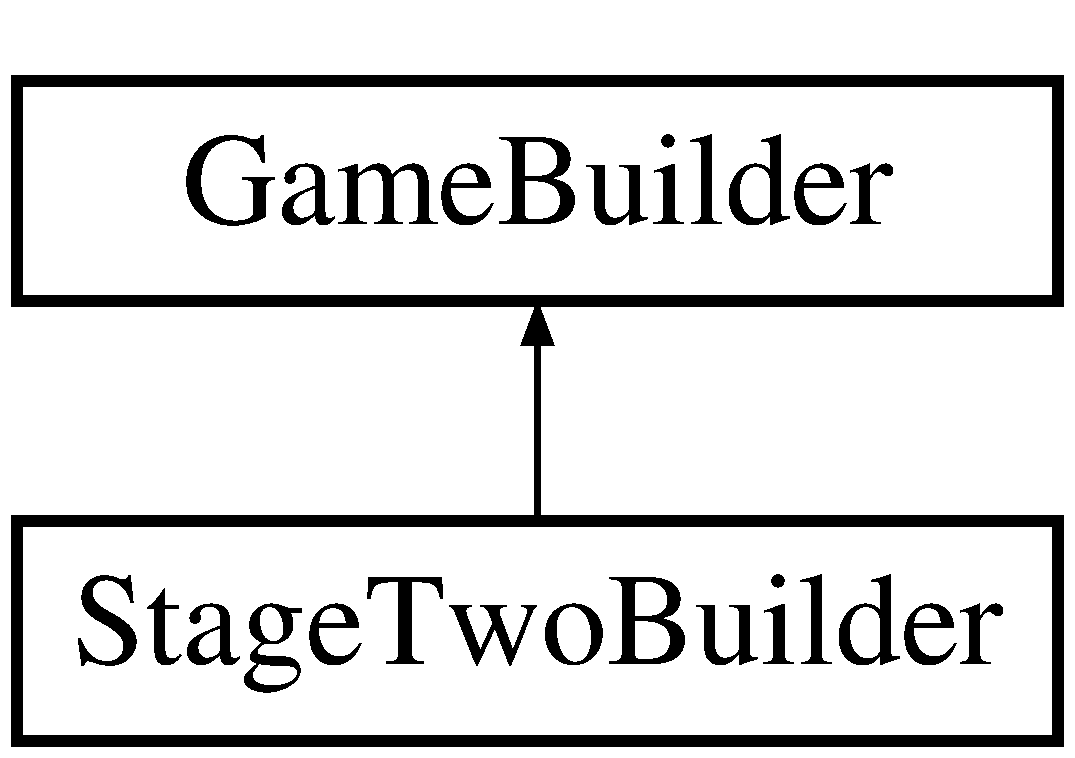
\includegraphics[height=2.000000cm]{class_stage_two_builder}
\end{center}
\end{figure}
\subsection*{Public Member Functions}
\begin{DoxyCompactItemize}
\item 
\mbox{\hyperlink{class_stage_two_builder_a46f9a84e6bde6ed8504f3c3f9bad71f3}{$\sim$\+Stage\+Two\+Builder}} ()
\item 
\mbox{\hyperlink{class_stage_two_builder_a1cf9558f9d7487a87ffae237c8546f8e}{Stage\+Two\+Builder}} ()
\item 
void \mbox{\hyperlink{class_stage_two_builder_a8b2b783294c26b5f40d16bdd54d86301}{add\+Ball}} (Q\+Json\+Object \&ball\+Data) override
\begin{DoxyCompactList}\small\item\em add\+Ball creates a ball to the current game being buil \end{DoxyCompactList}\item 
void \mbox{\hyperlink{class_stage_two_builder_a7326ee514e752cab6d994352f5ef68e0}{add\+Table}} (Q\+Json\+Object \&table\+Data) override
\begin{DoxyCompactList}\small\item\em add\+Table creates a table to the current game being built \end{DoxyCompactList}\item 
virtual \mbox{\hyperlink{class_game}{Game}} $\ast$ \mbox{\hyperlink{class_stage_two_builder_ac40c00c49b18b7c4f83f4474a8cd9c73}{get\+Result}} () override
\begin{DoxyCompactList}\small\item\em get\+Result -\/ retrieve the built object \end{DoxyCompactList}\end{DoxyCompactItemize}
\subsection*{Additional Inherited Members}


\subsection{Detailed Description}


Definition at line 7 of file stagetwobuilder.\+h.



\subsection{Constructor \& Destructor Documentation}
\mbox{\Hypertarget{class_stage_two_builder_a46f9a84e6bde6ed8504f3c3f9bad71f3}\label{class_stage_two_builder_a46f9a84e6bde6ed8504f3c3f9bad71f3}} 
\index{Stage\+Two\+Builder@{Stage\+Two\+Builder}!````~Stage\+Two\+Builder@{$\sim$\+Stage\+Two\+Builder}}
\index{````~Stage\+Two\+Builder@{$\sim$\+Stage\+Two\+Builder}!Stage\+Two\+Builder@{Stage\+Two\+Builder}}
\subsubsection{\texorpdfstring{$\sim$\+Stage\+Two\+Builder()}{~StageTwoBuilder()}}
{\footnotesize\ttfamily Stage\+Two\+Builder\+::$\sim$\+Stage\+Two\+Builder (\begin{DoxyParamCaption}{ }\end{DoxyParamCaption})\hspace{0.3cm}{\ttfamily [inline]}}



Definition at line 9 of file stagetwobuilder.\+h.

\mbox{\Hypertarget{class_stage_two_builder_a1cf9558f9d7487a87ffae237c8546f8e}\label{class_stage_two_builder_a1cf9558f9d7487a87ffae237c8546f8e}} 
\index{Stage\+Two\+Builder@{Stage\+Two\+Builder}!Stage\+Two\+Builder@{Stage\+Two\+Builder}}
\index{Stage\+Two\+Builder@{Stage\+Two\+Builder}!Stage\+Two\+Builder@{Stage\+Two\+Builder}}
\subsubsection{\texorpdfstring{Stage\+Two\+Builder()}{StageTwoBuilder()}}
{\footnotesize\ttfamily Stage\+Two\+Builder\+::\+Stage\+Two\+Builder (\begin{DoxyParamCaption}{ }\end{DoxyParamCaption})\hspace{0.3cm}{\ttfamily [inline]}}



Definition at line 10 of file stagetwobuilder.\+h.



\subsection{Member Function Documentation}
\mbox{\Hypertarget{class_stage_two_builder_a8b2b783294c26b5f40d16bdd54d86301}\label{class_stage_two_builder_a8b2b783294c26b5f40d16bdd54d86301}} 
\index{Stage\+Two\+Builder@{Stage\+Two\+Builder}!add\+Ball@{add\+Ball}}
\index{add\+Ball@{add\+Ball}!Stage\+Two\+Builder@{Stage\+Two\+Builder}}
\subsubsection{\texorpdfstring{add\+Ball()}{addBall()}}
{\footnotesize\ttfamily void Stage\+Two\+Builder\+::add\+Ball (\begin{DoxyParamCaption}\item[{Q\+Json\+Object \&}]{ball\+Data }\end{DoxyParamCaption})\hspace{0.3cm}{\ttfamily [override]}, {\ttfamily [virtual]}}



add\+Ball creates a ball to the current game being buil 


\begin{DoxyParams}{Parameters}
{\em ball\+Data} & -\/ json object that is simply an element of the array of balls provided in the config \\
\hline
\end{DoxyParams}


Implements \mbox{\hyperlink{class_game_builder_a836186637bd2f7844f7dfac0135d833b}{Game\+Builder}}.



Definition at line 140 of file stagetwobuilder.\+cpp.

\mbox{\Hypertarget{class_stage_two_builder_a7326ee514e752cab6d994352f5ef68e0}\label{class_stage_two_builder_a7326ee514e752cab6d994352f5ef68e0}} 
\index{Stage\+Two\+Builder@{Stage\+Two\+Builder}!add\+Table@{add\+Table}}
\index{add\+Table@{add\+Table}!Stage\+Two\+Builder@{Stage\+Two\+Builder}}
\subsubsection{\texorpdfstring{add\+Table()}{addTable()}}
{\footnotesize\ttfamily void Stage\+Two\+Builder\+::add\+Table (\begin{DoxyParamCaption}\item[{Q\+Json\+Object \&}]{table\+Data }\end{DoxyParamCaption})\hspace{0.3cm}{\ttfamily [override]}, {\ttfamily [virtual]}}



add\+Table creates a table to the current game being built 


\begin{DoxyParams}{Parameters}
{\em table\+Data} & -\/ json object that contains all properties of the table \\
\hline
\end{DoxyParams}


Implements \mbox{\hyperlink{class_game_builder_a65fb629009c18956a8d592352eda1eb5}{Game\+Builder}}.



Definition at line 207 of file stagetwobuilder.\+cpp.

\mbox{\Hypertarget{class_stage_two_builder_ac40c00c49b18b7c4f83f4474a8cd9c73}\label{class_stage_two_builder_ac40c00c49b18b7c4f83f4474a8cd9c73}} 
\index{Stage\+Two\+Builder@{Stage\+Two\+Builder}!get\+Result@{get\+Result}}
\index{get\+Result@{get\+Result}!Stage\+Two\+Builder@{Stage\+Two\+Builder}}
\subsubsection{\texorpdfstring{get\+Result()}{getResult()}}
{\footnotesize\ttfamily \mbox{\hyperlink{class_game}{Game}} $\ast$ Stage\+Two\+Builder\+::get\+Result (\begin{DoxyParamCaption}{ }\end{DoxyParamCaption})\hspace{0.3cm}{\ttfamily [override]}, {\ttfamily [virtual]}}



get\+Result -\/ retrieve the built object 

\begin{DoxyReturn}{Returns}

\end{DoxyReturn}


Reimplemented from \mbox{\hyperlink{class_game_builder_a490e3dbb7f8289edb2a080a3383f8607}{Game\+Builder}}.



Definition at line 230 of file stagetwobuilder.\+cpp.



The documentation for this class was generated from the following files\+:\begin{DoxyCompactItemize}
\item 
\mbox{\hyperlink{stagetwobuilder_8h}{stagetwobuilder.\+h}}\item 
\mbox{\hyperlink{stagetwobuilder_8cpp}{stagetwobuilder.\+cpp}}\end{DoxyCompactItemize}

\hypertarget{class_stage_two_factory}{}\section{Stage\+Two\+Factory Class Reference}
\label{class_stage_two_factory}\index{Stage\+Two\+Factory@{Stage\+Two\+Factory}}


Inherits \mbox{\hyperlink{class_abstract_stage_factory}{Abstract\+Stage\+Factory}}.

\subsection*{Public Member Functions}
\begin{DoxyCompactItemize}
\item 
virtual \mbox{\hyperlink{class_ball}{Ball}} $\ast$ \mbox{\hyperlink{class_stage_two_factory_aa12e02122eea28b08b3e148521bc2055}{make\+Ball}} (const Q\+Json\+Object \&ball\+Data) override
\begin{DoxyCompactList}\small\item\em make\+Ball -\/ construct a ball based on json \end{DoxyCompactList}\item 
virtual \mbox{\hyperlink{class_table}{Table}} $\ast$ \mbox{\hyperlink{class_stage_two_factory_aa532818e02bed0ea1f5c79a1a1487e71}{make\+Table}} (const Q\+Json\+Object \&table\+Data) override
\begin{DoxyCompactList}\small\item\em make\+Table -\/ construct a table based on json \end{DoxyCompactList}\item 
virtual \mbox{\hyperlink{class_pocket}{Pocket}} $\ast$ \mbox{\hyperlink{class_stage_two_factory_a6b66c413691103cf5df2840bcdb683ef}{make\+Pocket}} (const Q\+Json\+Object \&pocket\+Data) override
\begin{DoxyCompactList}\small\item\em make\+Pocket -\/ construct a pocket based on json \end{DoxyCompactList}\end{DoxyCompactItemize}


\subsection{Member Function Documentation}
\mbox{\Hypertarget{class_stage_two_factory_aa12e02122eea28b08b3e148521bc2055}\label{class_stage_two_factory_aa12e02122eea28b08b3e148521bc2055}} 
\index{Stage\+Two\+Factory@{Stage\+Two\+Factory}!make\+Ball@{make\+Ball}}
\index{make\+Ball@{make\+Ball}!Stage\+Two\+Factory@{Stage\+Two\+Factory}}
\subsubsection{\texorpdfstring{make\+Ball()}{makeBall()}}
{\footnotesize\ttfamily \mbox{\hyperlink{class_ball}{Ball}} $\ast$ Stage\+Two\+Factory\+::make\+Ball (\begin{DoxyParamCaption}\item[{const Q\+Json\+Object \&}]{ball\+Data }\end{DoxyParamCaption})\hspace{0.3cm}{\ttfamily [override]}, {\ttfamily [virtual]}}



make\+Ball -\/ construct a ball based on json 


\begin{DoxyParams}{Parameters}
{\em ball\+Data} & -\/ our json data for this table \\
\hline
\end{DoxyParams}
\begin{DoxyReturn}{Returns}

\end{DoxyReturn}


Implements \mbox{\hyperlink{class_abstract_stage_factory_a23367d64366e679aaff865620f5ce1ab}{Abstract\+Stage\+Factory}}.

\mbox{\Hypertarget{class_stage_two_factory_a6b66c413691103cf5df2840bcdb683ef}\label{class_stage_two_factory_a6b66c413691103cf5df2840bcdb683ef}} 
\index{Stage\+Two\+Factory@{Stage\+Two\+Factory}!make\+Pocket@{make\+Pocket}}
\index{make\+Pocket@{make\+Pocket}!Stage\+Two\+Factory@{Stage\+Two\+Factory}}
\subsubsection{\texorpdfstring{make\+Pocket()}{makePocket()}}
{\footnotesize\ttfamily \mbox{\hyperlink{class_pocket}{Pocket}} $\ast$ Stage\+Two\+Factory\+::make\+Pocket (\begin{DoxyParamCaption}\item[{const Q\+Json\+Object \&}]{pocket\+Data }\end{DoxyParamCaption})\hspace{0.3cm}{\ttfamily [override]}, {\ttfamily [virtual]}}



make\+Pocket -\/ construct a pocket based on json 


\begin{DoxyParams}{Parameters}
{\em pocket\+Data} & -\/ the json \\
\hline
\end{DoxyParams}
\begin{DoxyReturn}{Returns}
newly created pocket 
\end{DoxyReturn}


Implements \mbox{\hyperlink{class_abstract_stage_factory_a6ce57859e00b135049e3b995b7dfc94d}{Abstract\+Stage\+Factory}}.

\mbox{\Hypertarget{class_stage_two_factory_aa532818e02bed0ea1f5c79a1a1487e71}\label{class_stage_two_factory_aa532818e02bed0ea1f5c79a1a1487e71}} 
\index{Stage\+Two\+Factory@{Stage\+Two\+Factory}!make\+Table@{make\+Table}}
\index{make\+Table@{make\+Table}!Stage\+Two\+Factory@{Stage\+Two\+Factory}}
\subsubsection{\texorpdfstring{make\+Table()}{makeTable()}}
{\footnotesize\ttfamily \mbox{\hyperlink{class_table}{Table}} $\ast$ Stage\+Two\+Factory\+::make\+Table (\begin{DoxyParamCaption}\item[{const Q\+Json\+Object \&}]{table\+Data }\end{DoxyParamCaption})\hspace{0.3cm}{\ttfamily [override]}, {\ttfamily [virtual]}}



make\+Table -\/ construct a table based on json 


\begin{DoxyParams}{Parameters}
{\em table\+Data} & -\/ our json data for this table \\
\hline
\end{DoxyParams}
\begin{DoxyReturn}{Returns}

\end{DoxyReturn}


Implements \mbox{\hyperlink{class_abstract_stage_factory_a539c855ce9a09e08b7fcb3ffa7f0d3fd}{Abstract\+Stage\+Factory}}.



The documentation for this class was generated from the following files\+:\begin{DoxyCompactItemize}
\item 
stagetwofactory.\+h\item 
stagetwofactory.\+cpp\end{DoxyCompactItemize}

\hypertarget{class_stage_two_table}{}\section{Stage\+Two\+Table Class Reference}
\label{class_stage_two_table}\index{Stage\+Two\+Table@{Stage\+Two\+Table}}


Inherits \mbox{\hyperlink{class_table}{Table}}.

\subsection*{Public Member Functions}
\begin{DoxyCompactItemize}
\item 
\mbox{\Hypertarget{class_stage_two_table_abfe56f335f3eda0c72ae8477fe65e71f}\label{class_stage_two_table_abfe56f335f3eda0c72ae8477fe65e71f}} 
{\bfseries Stage\+Two\+Table} (int width, int height, Q\+Color colour, double friction)
\item 
void \mbox{\hyperlink{class_stage_two_table_ad19f7aa333b65d84b67ce2e55330a669}{render}} (Q\+Painter \&painter, const Q\+Vector2D \&offset) override
\begin{DoxyCompactList}\small\item\em render -\/ draw the stageonetable to screen using the specified painter \end{DoxyCompactList}\item 
\mbox{\Hypertarget{class_stage_two_table_a3e015671be449da741adaf86e00ec844}\label{class_stage_two_table_a3e015671be449da741adaf86e00ec844}} 
virtual bool {\bfseries sinks} (\mbox{\hyperlink{class_ball}{Ball}} $\ast$b) override
\item 
\mbox{\Hypertarget{class_stage_two_table_a0ee81cb52ee0caba2a68449409a63d10}\label{class_stage_two_table_a0ee81cb52ee0caba2a68449409a63d10}} 
void {\bfseries set\+Pockets} (std\+::vector$<$ \mbox{\hyperlink{class_pocket}{Pocket}} $\ast$$>$ pockets)
\item 
\mbox{\Hypertarget{class_stage_two_table_a13e9626ecbb5f84766efe7342e122873}\label{class_stage_two_table_a13e9626ecbb5f84766efe7342e122873}} 
void {\bfseries add\+Pocket} (\mbox{\hyperlink{class_pocket}{Pocket}} $\ast$p)
\item 
\mbox{\hyperlink{class_table}{Table}} $\ast$ \mbox{\hyperlink{class_stage_two_table_ab87e388ca2927670b37dffccb91a76b4}{copy}} () override
\begin{DoxyCompactList}\small\item\em copy deep copy the table \end{DoxyCompactList}\end{DoxyCompactItemize}
\subsection*{Protected Attributes}
\begin{DoxyCompactItemize}
\item 
\mbox{\Hypertarget{class_stage_two_table_aba6026e62b3894b57264b080e6a72b75}\label{class_stage_two_table_aba6026e62b3894b57264b080e6a72b75}} 
std\+::vector$<$ \mbox{\hyperlink{class_pocket}{Pocket}} $\ast$ $>$ {\bfseries m\+\_\+pockets}
\end{DoxyCompactItemize}


\subsection{Member Function Documentation}
\mbox{\Hypertarget{class_stage_two_table_ab87e388ca2927670b37dffccb91a76b4}\label{class_stage_two_table_ab87e388ca2927670b37dffccb91a76b4}} 
\index{Stage\+Two\+Table@{Stage\+Two\+Table}!copy@{copy}}
\index{copy@{copy}!Stage\+Two\+Table@{Stage\+Two\+Table}}
\subsubsection{\texorpdfstring{copy()}{copy()}}
{\footnotesize\ttfamily \mbox{\hyperlink{class_table}{Table}} $\ast$ Stage\+Two\+Table\+::copy (\begin{DoxyParamCaption}{ }\end{DoxyParamCaption})\hspace{0.3cm}{\ttfamily [override]}, {\ttfamily [virtual]}}



copy deep copy the table 

\begin{DoxyReturn}{Returns}
new table with different address 
\end{DoxyReturn}


Implements \mbox{\hyperlink{class_table_a881295d0bea9823026471422ec203c6e}{Table}}.

\mbox{\Hypertarget{class_stage_two_table_ad19f7aa333b65d84b67ce2e55330a669}\label{class_stage_two_table_ad19f7aa333b65d84b67ce2e55330a669}} 
\index{Stage\+Two\+Table@{Stage\+Two\+Table}!render@{render}}
\index{render@{render}!Stage\+Two\+Table@{Stage\+Two\+Table}}
\subsubsection{\texorpdfstring{render()}{render()}}
{\footnotesize\ttfamily void Stage\+Two\+Table\+::render (\begin{DoxyParamCaption}\item[{Q\+Painter \&}]{painter,  }\item[{const Q\+Vector2D \&}]{offset }\end{DoxyParamCaption})\hspace{0.3cm}{\ttfamily [override]}, {\ttfamily [virtual]}}



render -\/ draw the stageonetable to screen using the specified painter 


\begin{DoxyParams}{Parameters}
{\em painter} & -\/ painter to use \\
\hline
\end{DoxyParams}


Implements \mbox{\hyperlink{class_table_a827dac18920a95b3e0ef006183514654}{Table}}.



The documentation for this class was generated from the following files\+:\begin{DoxyCompactItemize}
\item 
table.\+h\item 
table.\+cpp\end{DoxyCompactItemize}

\hypertarget{class_table}{}\section{Table Class Reference}
\label{class_table}\index{Table@{Table}}


{\ttfamily \#include $<$table.\+h$>$}

Inheritance diagram for Table\+:\begin{figure}[H]
\begin{center}
\leavevmode
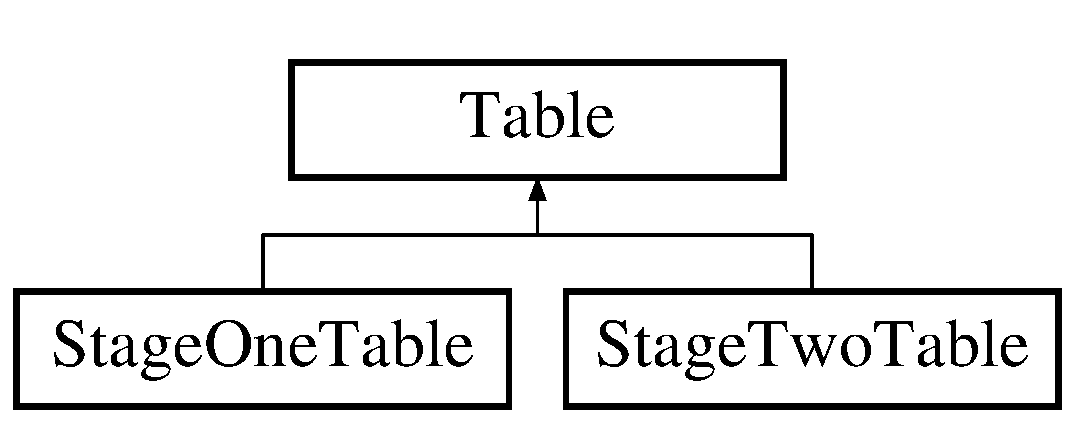
\includegraphics[height=2.000000cm]{class_table}
\end{center}
\end{figure}
\subsection*{Public Member Functions}
\begin{DoxyCompactItemize}
\item 
virtual \mbox{\hyperlink{class_table_ac7541d139723d710fb7c39b1898d6e87}{$\sim$\+Table}} ()
\item 
\mbox{\hyperlink{class_table_a7f7c9dbfd3a6ebf5360cfd30e6d9ceb6}{Table}} (int width, int height, Q\+Color colour, double friction)
\item 
virtual void \mbox{\hyperlink{class_table_a827dac18920a95b3e0ef006183514654}{render}} (Q\+Painter \&painter, const Q\+Vector2D \&offset)=0
\begin{DoxyCompactList}\small\item\em render -\/ draw the table to screen using the specified painter \end{DoxyCompactList}\item 
int \mbox{\hyperlink{class_table_a767798fbd671c4c6805091a116439444}{get\+Width}} () const
\item 
int \mbox{\hyperlink{class_table_a3c40550751e65b563b3f1759bd12985c}{get\+Height}} () const
\item 
double \mbox{\hyperlink{class_table_a250960dffeb3fa744bf098a49ef78d8a}{get\+Friction}} () const
\item 
virtual bool \mbox{\hyperlink{class_table_ab3eb192b2a06e26349d651e4e6de063a}{sinks}} (\mbox{\hyperlink{class_ball}{Ball}} $\ast$)
\end{DoxyCompactItemize}
\subsection*{Protected Attributes}
\begin{DoxyCompactItemize}
\item 
int \mbox{\hyperlink{class_table_a1e99922a6f86bbbe649c4705590b3409}{m\+\_\+width}}
\item 
int \mbox{\hyperlink{class_table_af1f22da42093769f53dcc3ebe7ea40c0}{m\+\_\+height}}
\item 
Q\+Brush \mbox{\hyperlink{class_table_a9c8db37610dfe62b570c7a386db69939}{m\+\_\+brush}}
\item 
double \mbox{\hyperlink{class_table_aa26465bb9074d6f07dec1a41a06a7d62}{m\+\_\+friction}}
\end{DoxyCompactItemize}


\subsection{Detailed Description}


Definition at line 10 of file table.\+h.



\subsection{Constructor \& Destructor Documentation}
\mbox{\Hypertarget{class_table_ac7541d139723d710fb7c39b1898d6e87}\label{class_table_ac7541d139723d710fb7c39b1898d6e87}} 
\index{Table@{Table}!````~Table@{$\sim$\+Table}}
\index{````~Table@{$\sim$\+Table}!Table@{Table}}
\subsubsection{\texorpdfstring{$\sim$\+Table()}{~Table()}}
{\footnotesize\ttfamily virtual Table\+::$\sim$\+Table (\begin{DoxyParamCaption}{ }\end{DoxyParamCaption})\hspace{0.3cm}{\ttfamily [inline]}, {\ttfamily [virtual]}}



Definition at line 17 of file table.\+h.

\mbox{\Hypertarget{class_table_a7f7c9dbfd3a6ebf5360cfd30e6d9ceb6}\label{class_table_a7f7c9dbfd3a6ebf5360cfd30e6d9ceb6}} 
\index{Table@{Table}!Table@{Table}}
\index{Table@{Table}!Table@{Table}}
\subsubsection{\texorpdfstring{Table()}{Table()}}
{\footnotesize\ttfamily Table\+::\+Table (\begin{DoxyParamCaption}\item[{int}]{width,  }\item[{int}]{height,  }\item[{Q\+Color}]{colour,  }\item[{double}]{friction }\end{DoxyParamCaption})\hspace{0.3cm}{\ttfamily [inline]}}



Definition at line 18 of file table.\+h.



\subsection{Member Function Documentation}
\mbox{\Hypertarget{class_table_a250960dffeb3fa744bf098a49ef78d8a}\label{class_table_a250960dffeb3fa744bf098a49ef78d8a}} 
\index{Table@{Table}!get\+Friction@{get\+Friction}}
\index{get\+Friction@{get\+Friction}!Table@{Table}}
\subsubsection{\texorpdfstring{get\+Friction()}{getFriction()}}
{\footnotesize\ttfamily double Table\+::get\+Friction (\begin{DoxyParamCaption}{ }\end{DoxyParamCaption}) const\hspace{0.3cm}{\ttfamily [inline]}}



Definition at line 29 of file table.\+h.

\mbox{\Hypertarget{class_table_a3c40550751e65b563b3f1759bd12985c}\label{class_table_a3c40550751e65b563b3f1759bd12985c}} 
\index{Table@{Table}!get\+Height@{get\+Height}}
\index{get\+Height@{get\+Height}!Table@{Table}}
\subsubsection{\texorpdfstring{get\+Height()}{getHeight()}}
{\footnotesize\ttfamily int Table\+::get\+Height (\begin{DoxyParamCaption}{ }\end{DoxyParamCaption}) const\hspace{0.3cm}{\ttfamily [inline]}}



Definition at line 28 of file table.\+h.

\mbox{\Hypertarget{class_table_a767798fbd671c4c6805091a116439444}\label{class_table_a767798fbd671c4c6805091a116439444}} 
\index{Table@{Table}!get\+Width@{get\+Width}}
\index{get\+Width@{get\+Width}!Table@{Table}}
\subsubsection{\texorpdfstring{get\+Width()}{getWidth()}}
{\footnotesize\ttfamily int Table\+::get\+Width (\begin{DoxyParamCaption}{ }\end{DoxyParamCaption}) const\hspace{0.3cm}{\ttfamily [inline]}}



Definition at line 27 of file table.\+h.

\mbox{\Hypertarget{class_table_a827dac18920a95b3e0ef006183514654}\label{class_table_a827dac18920a95b3e0ef006183514654}} 
\index{Table@{Table}!render@{render}}
\index{render@{render}!Table@{Table}}
\subsubsection{\texorpdfstring{render()}{render()}}
{\footnotesize\ttfamily virtual void Table\+::render (\begin{DoxyParamCaption}\item[{Q\+Painter \&}]{painter,  }\item[{const Q\+Vector2D \&}]{offset }\end{DoxyParamCaption})\hspace{0.3cm}{\ttfamily [pure virtual]}}



render -\/ draw the table to screen using the specified painter 


\begin{DoxyParams}{Parameters}
{\em painter} & -\/ painter to use \\
\hline
\end{DoxyParams}


Implemented in \mbox{\hyperlink{class_stage_two_table_ad19f7aa333b65d84b67ce2e55330a669}{Stage\+Two\+Table}}, and \mbox{\hyperlink{class_stage_one_table_a1f6dac59ce45c370f94fb3710f744ceb}{Stage\+One\+Table}}.

\mbox{\Hypertarget{class_table_ab3eb192b2a06e26349d651e4e6de063a}\label{class_table_ab3eb192b2a06e26349d651e4e6de063a}} 
\index{Table@{Table}!sinks@{sinks}}
\index{sinks@{sinks}!Table@{Table}}
\subsubsection{\texorpdfstring{sinks()}{sinks()}}
{\footnotesize\ttfamily virtual bool Table\+::sinks (\begin{DoxyParamCaption}\item[{\mbox{\hyperlink{class_ball}{Ball}} $\ast$}]{ }\end{DoxyParamCaption})\hspace{0.3cm}{\ttfamily [inline]}, {\ttfamily [virtual]}}



Reimplemented in \mbox{\hyperlink{class_stage_two_table_a3e015671be449da741adaf86e00ec844}{Stage\+Two\+Table}}.



Definition at line 31 of file table.\+h.



\subsection{Member Data Documentation}
\mbox{\Hypertarget{class_table_a9c8db37610dfe62b570c7a386db69939}\label{class_table_a9c8db37610dfe62b570c7a386db69939}} 
\index{Table@{Table}!m\+\_\+brush@{m\+\_\+brush}}
\index{m\+\_\+brush@{m\+\_\+brush}!Table@{Table}}
\subsubsection{\texorpdfstring{m\+\_\+brush}{m\_brush}}
{\footnotesize\ttfamily Q\+Brush Table\+::m\+\_\+brush\hspace{0.3cm}{\ttfamily [protected]}}



Definition at line 14 of file table.\+h.

\mbox{\Hypertarget{class_table_aa26465bb9074d6f07dec1a41a06a7d62}\label{class_table_aa26465bb9074d6f07dec1a41a06a7d62}} 
\index{Table@{Table}!m\+\_\+friction@{m\+\_\+friction}}
\index{m\+\_\+friction@{m\+\_\+friction}!Table@{Table}}
\subsubsection{\texorpdfstring{m\+\_\+friction}{m\_friction}}
{\footnotesize\ttfamily double Table\+::m\+\_\+friction\hspace{0.3cm}{\ttfamily [protected]}}



Definition at line 15 of file table.\+h.

\mbox{\Hypertarget{class_table_af1f22da42093769f53dcc3ebe7ea40c0}\label{class_table_af1f22da42093769f53dcc3ebe7ea40c0}} 
\index{Table@{Table}!m\+\_\+height@{m\+\_\+height}}
\index{m\+\_\+height@{m\+\_\+height}!Table@{Table}}
\subsubsection{\texorpdfstring{m\+\_\+height}{m\_height}}
{\footnotesize\ttfamily int Table\+::m\+\_\+height\hspace{0.3cm}{\ttfamily [protected]}}



Definition at line 13 of file table.\+h.

\mbox{\Hypertarget{class_table_a1e99922a6f86bbbe649c4705590b3409}\label{class_table_a1e99922a6f86bbbe649c4705590b3409}} 
\index{Table@{Table}!m\+\_\+width@{m\+\_\+width}}
\index{m\+\_\+width@{m\+\_\+width}!Table@{Table}}
\subsubsection{\texorpdfstring{m\+\_\+width}{m\_width}}
{\footnotesize\ttfamily int Table\+::m\+\_\+width\hspace{0.3cm}{\ttfamily [protected]}}



Definition at line 12 of file table.\+h.



The documentation for this class was generated from the following file\+:\begin{DoxyCompactItemize}
\item 
\mbox{\hyperlink{table_8h}{table.\+h}}\end{DoxyCompactItemize}

\chapter{File Documentation}
\hypertarget{abstractstagefactory_8h}{}\section{abstractstagefactory.\+h File Reference}
\label{abstractstagefactory_8h}\index{abstractstagefactory.\+h@{abstractstagefactory.\+h}}
{\ttfamily \#include \char`\"{}ball.\+h\char`\"{}}\newline
{\ttfamily \#include \char`\"{}table.\+h\char`\"{}}\newline
{\ttfamily \#include \char`\"{}pocket.\+h\char`\"{}}\newline
\subsection*{Classes}
\begin{DoxyCompactItemize}
\item 
class \mbox{\hyperlink{class_abstract_stage_factory}{Abstract\+Stage\+Factory}}
\end{DoxyCompactItemize}

\hypertarget{ball_8cpp}{}\section{ball.\+cpp File Reference}
\label{ball_8cpp}\index{ball.\+cpp@{ball.\+cpp}}
{\ttfamily \#include \char`\"{}ball.\+h\char`\"{}}\newline
{\ttfamily \#include $<$iostream$>$}\newline

\hypertarget{ball_8h}{}\section{ball.\+h File Reference}
\label{ball_8h}\index{ball.\+h@{ball.\+h}}
{\ttfamily \#include $<$Q\+Point$>$}\newline
{\ttfamily \#include $<$cmath$>$}\newline
{\ttfamily \#include $<$Q\+Painter$>$}\newline
{\ttfamily \#include $<$Q\+Vector2D$>$}\newline
\subsection*{Classes}
\begin{DoxyCompactItemize}
\item 
class \mbox{\hyperlink{class_ball}{Ball}}
\item 
class \mbox{\hyperlink{class_stage_one_ball}{Stage\+One\+Ball}}
\item 
class \mbox{\hyperlink{class_composite_ball}{Composite\+Ball}}
\end{DoxyCompactItemize}

\hypertarget{balldecorator_8cpp}{}\section{balldecorator.\+cpp File Reference}
\label{balldecorator_8cpp}\index{balldecorator.\+cpp@{balldecorator.\+cpp}}
{\ttfamily \#include \char`\"{}balldecorator.\+h\char`\"{}}\newline

\hypertarget{balldecorator_8h}{}\section{balldecorator.\+h File Reference}
\label{balldecorator_8h}\index{balldecorator.\+h@{balldecorator.\+h}}
{\ttfamily \#include \char`\"{}ball.\+h\char`\"{}}\newline
\subsection*{Classes}
\begin{DoxyCompactItemize}
\item 
class \mbox{\hyperlink{class_ball_decorator}{Ball\+Decorator}}
\begin{DoxyCompactList}\small\item\em The \mbox{\hyperlink{class_ball_decorator}{Ball\+Decorator}} class This acts as a Decorator. Any methods not overriden can simply forward the requests onto the Class this is decorated. \end{DoxyCompactList}\item 
class \mbox{\hyperlink{class_cue_ball}{Cue\+Ball}}
\begin{DoxyCompactList}\small\item\em The \mbox{\hyperlink{class_cue_ball}{Cue\+Ball}} class This handles some mouse interactions, and can control the position/velocity of the ball The ball will only be able to be controlled if the mouse click\&drag event originated at the position of the cue ball. \end{DoxyCompactList}\item 
class \mbox{\hyperlink{class_ball_sparkle_decorator}{Ball\+Sparkle\+Decorator}}
\item 
struct \mbox{\hyperlink{struct_ball_sparkle_decorator_1_1_sparkle}{Ball\+Sparkle\+Decorator\+::\+Sparkle}}
\item 
class \mbox{\hyperlink{class_ball_smash_decorator}{Ball\+Smash\+Decorator}}
\item 
struct \mbox{\hyperlink{struct_ball_smash_decorator_1_1_crumb}{Ball\+Smash\+Decorator\+::\+Crumb}}
\end{DoxyCompactItemize}

\hypertarget{dialog_8cpp}{}\section{dialog.\+cpp File Reference}
\label{dialog_8cpp}\index{dialog.\+cpp@{dialog.\+cpp}}
{\ttfamily \#include \char`\"{}dialog.\+h\char`\"{}}\newline
{\ttfamily \#include \char`\"{}ui\+\_\+dialog.\+h\char`\"{}}\newline
{\ttfamily \#include $<$Q\+Painter$>$}\newline
{\ttfamily \#include $<$Q\+Timer$>$}\newline
{\ttfamily \#include $<$iostream$>$}\newline
{\ttfamily \#include $<$Q\+Mouse\+Event$>$}\newline
{\ttfamily \#include \char`\"{}utils.\+h\char`\"{}}\newline

\hypertarget{dialog_8h}{}\section{dialog.\+h File Reference}
\label{dialog_8h}\index{dialog.\+h@{dialog.\+h}}
{\ttfamily \#include $<$Q\+Dialog$>$}\newline
{\ttfamily \#include \char`\"{}ball.\+h\char`\"{}}\newline
{\ttfamily \#include \char`\"{}game.\+h\char`\"{}}\newline
\subsection*{Classes}
\begin{DoxyCompactItemize}
\item 
class \mbox{\hyperlink{class_dialog}{Dialog}}
\end{DoxyCompactItemize}
\subsection*{Namespaces}
\begin{DoxyCompactItemize}
\item 
 \mbox{\hyperlink{namespace_ui}{Ui}}
\end{DoxyCompactItemize}

\hypertarget{game_8cpp}{}\section{game.\+cpp File Reference}
\label{game_8cpp}\index{game.\+cpp@{game.\+cpp}}
{\ttfamily \#include \char`\"{}game.\+h\char`\"{}}\newline
{\ttfamily \#include \char`\"{}utils.\+h\char`\"{}}\newline
{\ttfamily \#include $<$Q\+Json\+Array$>$}\newline
{\ttfamily \#include $<$stdexcept$>$}\newline
{\ttfamily \#include $<$cmath$>$}\newline
{\ttfamily \#include $<$exception$>$}\newline
{\ttfamily \#include $<$iostream$>$}\newline

\hypertarget{game_8h}{}\section{game.\+h File Reference}
\label{game_8h}\index{game.\+h@{game.\+h}}
{\ttfamily \#include $<$Q\+Json\+Object$>$}\newline
{\ttfamily \#include \char`\"{}abstractstagefactory.\+h\char`\"{}}\newline
{\ttfamily \#include \char`\"{}table.\+h\char`\"{}}\newline
{\ttfamily \#include \char`\"{}ball.\+h\char`\"{}}\newline
{\ttfamily \#include \char`\"{}balldecorator.\+h\char`\"{}}\newline
\subsection*{Classes}
\begin{DoxyCompactItemize}
\item 
class \mbox{\hyperlink{class_game}{Game}}
\end{DoxyCompactItemize}

\hypertarget{gamebuilder_8cpp}{}\section{gamebuilder.\+cpp File Reference}
\label{gamebuilder_8cpp}\index{gamebuilder.\+cpp@{gamebuilder.\+cpp}}
{\ttfamily \#include \char`\"{}gamebuilder.\+h\char`\"{}}\newline
{\ttfamily \#include \char`\"{}game.\+h\char`\"{}}\newline
{\ttfamily \#include \char`\"{}utils.\+h\char`\"{}}\newline
{\ttfamily \#include $<$iostream$>$}\newline
{\ttfamily \#include $<$functional$>$}\newline
{\ttfamily \#include $<$Q\+Json\+Array$>$}\newline

\hypertarget{gamebuilder_8h}{}\section{gamebuilder.\+h File Reference}
\label{gamebuilder_8h}\index{gamebuilder.\+h@{gamebuilder.\+h}}
{\ttfamily \#include \char`\"{}stageonefactory.\+h\char`\"{}}\newline
{\ttfamily \#include \char`\"{}stagetwofactory.\+h\char`\"{}}\newline
{\ttfamily \#include \char`\"{}game.\+h\char`\"{}}\newline
\subsection*{Classes}
\begin{DoxyCompactItemize}
\item 
class \mbox{\hyperlink{class_game_builder}{Game\+Builder}}
\item 
class \mbox{\hyperlink{class_stage_one_builder}{Stage\+One\+Builder}}
\item 
class \mbox{\hyperlink{class_game_director}{Game\+Director}}
\end{DoxyCompactItemize}

\hypertarget{main_8cpp}{}\section{main.\+cpp File Reference}
\label{main_8cpp}\index{main.\+cpp@{main.\+cpp}}
{\ttfamily \#include \char`\"{}dialog.\+h\char`\"{}}\newline
{\ttfamily \#include \char`\"{}game.\+h\char`\"{}}\newline
{\ttfamily \#include \char`\"{}utils.\+h\char`\"{}}\newline
{\ttfamily \#include \char`\"{}gamebuilder.\+h\char`\"{}}\newline
{\ttfamily \#include \char`\"{}stagetwobuilder.\+h\char`\"{}}\newline
{\ttfamily \#include $<$Q\+Application$>$}\newline
{\ttfamily \#include $<$Q\+File$>$}\newline
{\ttfamily \#include $<$iostream$>$}\newline
{\ttfamily \#include $<$Q\+String$>$}\newline
{\ttfamily \#include $<$Q\+Json\+Object$>$}\newline
{\ttfamily \#include $<$ctime$>$}\newline
{\ttfamily \#include $<$Q\+Json\+Document$>$}\newline
\subsection*{Functions}
\begin{DoxyCompactItemize}
\item 
Q\+Json\+Object \mbox{\hyperlink{main_8cpp_a37efa081d531cc5d8da08d21cb302ae1}{load\+Config}} ()
\item 
int \mbox{\hyperlink{main_8cpp_a0ddf1224851353fc92bfbff6f499fa97}{main}} (int argc, char $\ast$argv\mbox{[}$\,$\mbox{]})
\end{DoxyCompactItemize}


\subsection{Function Documentation}
\mbox{\Hypertarget{main_8cpp_a37efa081d531cc5d8da08d21cb302ae1}\label{main_8cpp_a37efa081d531cc5d8da08d21cb302ae1}} 
\index{main.\+cpp@{main.\+cpp}!load\+Config@{load\+Config}}
\index{load\+Config@{load\+Config}!main.\+cpp@{main.\+cpp}}
\subsubsection{\texorpdfstring{load\+Config()}{loadConfig()}}
{\footnotesize\ttfamily Q\+Json\+Object load\+Config (\begin{DoxyParamCaption}{ }\end{DoxyParamCaption})}

Written by Tim Burr 2018/05/18 

Definition at line 19 of file main.\+cpp.

\mbox{\Hypertarget{main_8cpp_a0ddf1224851353fc92bfbff6f499fa97}\label{main_8cpp_a0ddf1224851353fc92bfbff6f499fa97}} 
\index{main.\+cpp@{main.\+cpp}!main@{main}}
\index{main@{main}!main.\+cpp@{main.\+cpp}}
\subsubsection{\texorpdfstring{main()}{main()}}
{\footnotesize\ttfamily int main (\begin{DoxyParamCaption}\item[{int}]{argc,  }\item[{char $\ast$}]{argv\mbox{[}$\,$\mbox{]} }\end{DoxyParamCaption})}



Definition at line 29 of file main.\+cpp.


\hypertarget{pocket_8cpp}{}\section{pocket.\+cpp File Reference}
\label{pocket_8cpp}\index{pocket.\+cpp@{pocket.\+cpp}}
{\ttfamily \#include \char`\"{}pocket.\+h\char`\"{}}\newline

\hypertarget{pocket_8h}{}\section{pocket.\+h File Reference}
\label{pocket_8h}\index{pocket.\+h@{pocket.\+h}}
{\ttfamily \#include $<$Q\+Vector2D$>$}\newline
{\ttfamily \#include $<$Q\+Painter$>$}\newline
{\ttfamily \#include $<$Q\+Brush$>$}\newline
{\ttfamily \#include $<$cmath$>$}\newline
\subsection*{Classes}
\begin{DoxyCompactItemize}
\item 
class \mbox{\hyperlink{class_pocket}{Pocket}}
\end{DoxyCompactItemize}

\hypertarget{stageonefactory_8cpp}{}\section{stageonefactory.\+cpp File Reference}
\label{stageonefactory_8cpp}\index{stageonefactory.\+cpp@{stageonefactory.\+cpp}}
{\ttfamily \#include \char`\"{}stageonefactory.\+h\char`\"{}}\newline
{\ttfamily \#include $<$Q\+Json\+Object$>$}\newline

\hypertarget{stageonefactory_8h}{}\section{stageonefactory.\+h File Reference}
\label{stageonefactory_8h}\index{stageonefactory.\+h@{stageonefactory.\+h}}
{\ttfamily \#include \char`\"{}abstractstagefactory.\+h\char`\"{}}\newline
\subsection*{Classes}
\begin{DoxyCompactItemize}
\item 
class \mbox{\hyperlink{class_stage_one_factory}{Stage\+One\+Factory}}
\end{DoxyCompactItemize}

\hypertarget{stagetwobuilder_8cpp}{}\section{stagetwobuilder.\+cpp File Reference}
\label{stagetwobuilder_8cpp}\index{stagetwobuilder.\+cpp@{stagetwobuilder.\+cpp}}
{\ttfamily \#include \char`\"{}stagetwobuilder.\+h\char`\"{}}\newline
{\ttfamily \#include \char`\"{}utils.\+h\char`\"{}}\newline
{\ttfamily \#include $<$iostream$>$}\newline
{\ttfamily \#include $<$Q\+Json\+Array$>$}\newline
{\ttfamily \#include $<$cassert$>$}\newline
{\ttfamily \#include $<$functional$>$}\newline
{\ttfamily \#include \char`\"{}ball.\+h\char`\"{}}\newline

\hypertarget{stagetwobuilder_8h}{}\section{stagetwobuilder.\+h File Reference}
\label{stagetwobuilder_8h}\index{stagetwobuilder.\+h@{stagetwobuilder.\+h}}
{\ttfamily \#include \char`\"{}gamebuilder.\+h\char`\"{}}\newline
{\ttfamily \#include \char`\"{}utils.\+h\char`\"{}}\newline
{\ttfamily \#include $<$iostream$>$}\newline
\subsection*{Classes}
\begin{DoxyCompactItemize}
\item 
class \mbox{\hyperlink{class_stage_two_builder}{Stage\+Two\+Builder}}
\end{DoxyCompactItemize}

\hypertarget{stagetwofactory_8cpp}{}\section{stagetwofactory.\+cpp File Reference}
\label{stagetwofactory_8cpp}\index{stagetwofactory.\+cpp@{stagetwofactory.\+cpp}}
{\ttfamily \#include \char`\"{}stagetwofactory.\+h\char`\"{}}\newline
{\ttfamily \#include $<$iostream$>$}\newline

\hypertarget{stagetwofactory_8h}{}\section{stagetwofactory.\+h File Reference}
\label{stagetwofactory_8h}\index{stagetwofactory.\+h@{stagetwofactory.\+h}}
{\ttfamily \#include \char`\"{}abstractstagefactory.\+h\char`\"{}}\newline
{\ttfamily \#include $<$Q\+Json\+Object$>$}\newline
\subsection*{Classes}
\begin{DoxyCompactItemize}
\item 
class \mbox{\hyperlink{class_stage_two_factory}{Stage\+Two\+Factory}}
\end{DoxyCompactItemize}

\hypertarget{table_8cpp}{}\section{table.\+cpp File Reference}
\label{table_8cpp}\index{table.\+cpp@{table.\+cpp}}
{\ttfamily \#include \char`\"{}table.\+h\char`\"{}}\newline
{\ttfamily \#include \char`\"{}ball.\+h\char`\"{}}\newline
{\ttfamily \#include $<$iostream$>$}\newline

\hypertarget{table_8h}{}\section{table.\+h File Reference}
\label{table_8h}\index{table.\+h@{table.\+h}}
{\ttfamily \#include $<$Q\+Color$>$}\newline
{\ttfamily \#include $<$Q\+Painter$>$}\newline
{\ttfamily \#include \char`\"{}pocket.\+h\char`\"{}}\newline
\subsection*{Classes}
\begin{DoxyCompactItemize}
\item 
class \mbox{\hyperlink{class_table}{Table}}
\item 
class \mbox{\hyperlink{class_stage_one_table}{Stage\+One\+Table}}
\item 
class \mbox{\hyperlink{class_stage_two_table}{Stage\+Two\+Table}}
\end{DoxyCompactItemize}

\hypertarget{utils_8h}{}\section{utils.\+h File Reference}
\label{utils_8h}\index{utils.\+h@{utils.\+h}}
{\ttfamily \#include $<$Q\+Vector2D$>$}\newline
{\ttfamily \#include $<$limits$>$}\newline
\subsection*{Variables}
\begin{DoxyCompactItemize}
\item 
constexpr char \mbox{\hyperlink{utils_8h_a1aff699eae47d9fa6fe4cf7dbc13eb0f}{config\+\_\+path}} \mbox{[}$\,$\mbox{]} = \char`\"{}config.\+json\char`\"{}
\item 
constexpr int \mbox{\hyperlink{utils_8h_a98a7326f78465e4b4de3271285aae66d}{anim\+Frame\+MS}} = 16
\item 
constexpr int \mbox{\hyperlink{utils_8h_a51dda64bc6c1218767343462e8994aa0}{draw\+Frame\+MS}} = 16
\item 
constexpr double \mbox{\hyperlink{utils_8h_a886ca5636b50114abd8205e7b11b7f97}{D\+O\+U\+B\+L\+E\+I\+NF}} = std\+::numeric\+\_\+limits$<$double$>$\+::max()
\end{DoxyCompactItemize}


\subsection{Variable Documentation}
\mbox{\Hypertarget{utils_8h_a98a7326f78465e4b4de3271285aae66d}\label{utils_8h_a98a7326f78465e4b4de3271285aae66d}} 
\index{utils.\+h@{utils.\+h}!anim\+Frame\+MS@{anim\+Frame\+MS}}
\index{anim\+Frame\+MS@{anim\+Frame\+MS}!utils.\+h@{utils.\+h}}
\subsubsection{\texorpdfstring{anim\+Frame\+MS}{animFrameMS}}
{\footnotesize\ttfamily constexpr int anim\+Frame\+MS = 16}



Definition at line 9 of file utils.\+h.

\mbox{\Hypertarget{utils_8h_a1aff699eae47d9fa6fe4cf7dbc13eb0f}\label{utils_8h_a1aff699eae47d9fa6fe4cf7dbc13eb0f}} 
\index{utils.\+h@{utils.\+h}!config\+\_\+path@{config\+\_\+path}}
\index{config\+\_\+path@{config\+\_\+path}!utils.\+h@{utils.\+h}}
\subsubsection{\texorpdfstring{config\+\_\+path}{config\_path}}
{\footnotesize\ttfamily constexpr char config\+\_\+path\mbox{[}$\,$\mbox{]} = \char`\"{}config.\+json\char`\"{}}



Definition at line 7 of file utils.\+h.

\mbox{\Hypertarget{utils_8h_a886ca5636b50114abd8205e7b11b7f97}\label{utils_8h_a886ca5636b50114abd8205e7b11b7f97}} 
\index{utils.\+h@{utils.\+h}!D\+O\+U\+B\+L\+E\+I\+NF@{D\+O\+U\+B\+L\+E\+I\+NF}}
\index{D\+O\+U\+B\+L\+E\+I\+NF@{D\+O\+U\+B\+L\+E\+I\+NF}!utils.\+h@{utils.\+h}}
\subsubsection{\texorpdfstring{D\+O\+U\+B\+L\+E\+I\+NF}{DOUBLEINF}}
{\footnotesize\ttfamily constexpr double D\+O\+U\+B\+L\+E\+I\+NF = std\+::numeric\+\_\+limits$<$double$>$\+::max()}



Definition at line 12 of file utils.\+h.

\mbox{\Hypertarget{utils_8h_a51dda64bc6c1218767343462e8994aa0}\label{utils_8h_a51dda64bc6c1218767343462e8994aa0}} 
\index{utils.\+h@{utils.\+h}!draw\+Frame\+MS@{draw\+Frame\+MS}}
\index{draw\+Frame\+MS@{draw\+Frame\+MS}!utils.\+h@{utils.\+h}}
\subsubsection{\texorpdfstring{draw\+Frame\+MS}{drawFrameMS}}
{\footnotesize\ttfamily constexpr int draw\+Frame\+MS = 16}



Definition at line 10 of file utils.\+h.


%--- End generated contents ---

% Index
\backmatter
\newpage
\phantomsection
\clearemptydoublepage
\addcontentsline{toc}{chapter}{Index}
\printindex

\end{document}
